\documentclass[10pt,letterpaper]{article}
\usepackage[margin=1in]{geometry}
\usepackage[T1]{fontenc}
\usepackage{textcomp,times,mathptmx,amsmath,amssymb,amsthm,booktabs,longtable,graphicx,float}
\usepackage{algorithm}
\usepackage[noend]{algpseudocode}
\usepackage[hidelinks]{hyperref}
\usepackage{cite}
\setlength{\emergencystretch}{1em}
\newtheorem{lemma}{Lemma}[section]
\newtheorem{proposition}[lemma]{Proposition}
\newtheorem{theorem}[lemma]{Theorem}
\newtheorem{corollary}[lemma]{Corollary}
\theoremstyle{remark}\newtheorem{remark}[lemma]{Remark}
\newcommand{\free}{\mathrm{free}}
\newcommand{\dtop}{d_{\mathrm{top}}}
\newcommand{\lca}{\mathrm{lca}}
\renewcommand{\thesection}{S\arabic{section}}
\renewcommand{\thefigure}{S\arabic{figure}}
\renewcommand{\thetable}{S\arabic{table}}
\renewcommand{\theequation}{S\arabic{equation}}
\title{Reference-Guided Merge Tree Maps:\\A Unified Position--Topology Framework\\Supplementary Material}
\author{Anonymous Authors}\date{}
\makeatletter
\renewcommand*\l@section{\@dottedtocline{1}{0em}{2.6em}}
\makeatother
\begin{document}\maketitle
This supplement provides derivations, algorithms, data protocols, complete metrics, controls, and reproducibility details. The five-sequence planar temporal evaluation (614 frames), independent mirror-motion control (64 frames), original-grid Tangaroa and Cylinder sequences (201 and 102 volumes), static Nucleon slice, and reconstructed Benzene potential (21 static sections) are separate experimental populations. The 744-hour Storms overview is a visualization-only experiment. Standard-metric re-evaluation covers all nine inputs, including 325 subsequently computed ST-MTM layouts. It is reported separately from the retained primary anchor-based metrics; physical temporal TD and static adjacent-section displacement are distinguished.

S1--S3 establish the formal model, planar protocols, and validation; S4 retains additional visuals; S5 records reproducibility. S6 details Tangaroa, S7 audits the event cases and baselines, S8 records figure coordinates and aggregations, S9 documents the additional inputs, and S10 collects complete visual comparisons. The main figures retain their source arrays and scalar scales; full-resolution profiles, rather than figure previews, supply the reported errors.
\begingroup\small\tableofcontents\endgroup\clearpage
\section{Formal Derivations and Algorithms}
The main paper presents one four-term interval model, its parameter regimes, a feasibility oracle, and a retained eligibility-based construction. The workflow figure illustrates the latter policy. This section retains the full interval constraints, closed-form costs, frontier definition, display-grid recurrence, and detailed planar construction; S2 specifies the quadratic objective, and S6 records the large-tree bounds and candidate-search protocol.
\subsection{Unified model: regimes, constraints and feasibility}\label{supp:framework}
The main model uses the same interval widths, canvas, variable set, four-term layout objective and source-value renderer in every operating regime. Native TMTM and ST-MTM are comparison methods. The topology--time and topology--geometry regimes express their design priorities without changing to their representations or pipelines.

\paragraph{Objective restrictions.}
For a fixed order, ordered distances are linear signed differences. Each term is a nonnegative sum of squared affine residuals, so the constrained layout is convex. Zeroing a weight removes that residual; it leaves any separate hard constraints intact. With $\lambda_R=0$, $B=\infty$ and $\eta=0$, both the feasible set and objective are independent of the values of $q$ at fixed canvas, geometry and candidate pool. A free translation is fixed using the canvas centre. A candidate pool that changes when $q$ changes can still change the searched orders; the invariance claim is conditional on the same pool.

The temporal target $p_i+\eta(q_i^t-q_i^{t-1})$ continuously interpolates stationary alignment and projected-motion following. At $\eta=0$ and fixed order, the geometry-plus-time objective has the stress/anchor form used by ST-MTM, but mean normalization, weight ratios, fixed widths, canvas boundaries and eccentricity regularization are declared differences. The topology--time mode is an anchor-level temporal-alignment surrogate, not TMTM's all-subtree overlap energy.

\paragraph{Removing the hidden reference constraint.}
The retained construction sets an automatic allowance $\tau^*+\beta$. Even at zero reference weight this cap still controls the positions. For two supports at distance 10 with references 20 and 100, widths 6, gap 1, canvas length 120 and $\beta=1$, the old cap gives anchors 21 and 99. Explicitly disabling it allows a distance of 10 and a canvas-centred mean of 60. This is a numerical regression test, not an application-data result. The historical default remains available for the retained P/R construction.

\paragraph{Scalar-budget solver.}
For order $\pi$, let $P_{ij}$ be the source merge level, $C_k=\min_{i\le k<j}P_{ij}$, and $\ell_k=\max(f_{\pi_k},f_{\pi_{k+1}})$ in join convention. The minimum labelled error is
\[
\delta^*(\pi)=\max\left(0,\max_k(\ell_k-C_k),\max_{i<j}\frac{P_{ij}-\max_{i\le k<j}C_k}{2}\right).
\]
The witness barriers are $C_k+\delta^*(\pi)$. The position cost follows the interval-window formula derived below. Exhaustively enumerating permutations and rejecting $\delta^*>\varepsilon\Delta_F$ and $\tau>BL$ yields the exact continuous feasibility answer. Minimizing the remaining $\tau$ gives the reference frontier; minimizing the QP objective instead gives a design compromise within the same admissible set.

\paragraph{Nested sets and endpoints.}
For $\varepsilon_1\le\varepsilon_2$, every order admitted at $\varepsilon_1$ is admitted at $\varepsilon_2$. This proves non-increasing optimal reference error for all permutations or a fixed candidate pool. Increasing a position allowance similarly cannot increase the least required scalar error. With fixed preceding anchors and weights, the optimum of the composite objective also cannot increase. Sequential histories may differ across a sweep, so this last statement is not a monotonicity guarantee for the recomputed temporal sequence or any individual component score.

At zero scalar allowance, only zero-error orders are admitted; with distinct branching values these are the hierarchy-compatible orders. An unrestricted allowance admits every order. Candidate-only searches retain nesting within their pools but not a full-space optimality or global infeasibility guarantee.

\paragraph{Three-leaf transition.}
For leaves $A,B,C$ of value zero, source merges $P_{AB}=1$ and $P_{AC}=P_{BC}=3$, the order $A,C,B$ requires $\delta^*=1$. With references $(1,9,5)$ for $(A,B,C)$, widths $0.2$, gap $0.1$, a canvas of length 10, and zero eccentricity, the topology-preserving minimax displacement is 2.15. A scalar allowance below 1 excludes the reference order; at allowance 1, zero position error becomes feasible. The critical normalized allowance is $1/3$ for scalar range 3. A requested zero position error below this allowance is infeasible.

\paragraph{Reproducibility and independent evidence.}
The common-QP runner and exporter are in \path{experiments/unified/}; complete controls, per-frame inputs, candidate pools, QP witnesses, native similarity controls and scalar maps are in \path{results/unified20261025/}. Native comparison is descriptive similarity after one sequence-wide affine gauge fit including reflection, with no framewise fitting. Pair-order agreement and anchor RMSE are reported separately. Results are not used to tune parameters toward native output equality.

The independent exhaustive frontier experiment remains in \path{experiments/framework/} and \path{results/framework20261025/}: 614 frames, 603 exhaustive and 11 candidate-only, nine topology settings, 5526 witnesses and 3684 inverse queries. Its historical native-wrapper comparison is an interface regression, not evidence for unification. Seven new tests check reference deactivation, temporal interpolation, scalar transitions, fixed-history objective nesting, track matching, infeasibility, search-coverage reporting and canonical placement in objective null spaces. The complete suite now contains 57 tests.

Strict-extremum clearance and raster rounding require separate measured-error checks. The analytical guarantees refer to continuous non-strict profiles. The historical P/R eligibility settings and their measured application results remain separate from the new true-error budgets and common-QP experiments.

\subsection{Assumptions and feasible layouts}
A rooted tree $T$ with leaves $1,\dots,n$; \emph{branching} nodes have $\ge 2$ children (unary chains contracted); $p(v)$ is the parent of a non-root branching node $v$ and $S_v$ its leaf set. Join-tree convention: $f$ strictly increases along root-ward paths; leaves are minima (split trees: negate $f$).
Leaf $i$ has reference $q_i\in\mathbb R$, width $w_i>0$, eccentricity radius $h_i=\rho w_i/2$ with $\rho\in[0,1]$; gap $g>0$; canvas $[a,a+L]$.
A layout $(\pi,z,u)$ satisfies
(D) $z_y-z_x\ge (w_x+w_y)/2+g$ for $\pi$-consecutive $x,y$;
(C) $a+w_i/2\le z_i\le a+L-w_i/2$;
(E) $|u_i-z_i|\le h_i$.
Assume $\sum_iw_i+(n-1)g\le L$ so the feasible set is nonempty.
$\Pi(T)$: orders in which every $S_v$ is contiguous.
$\tau(\pi)=\min_{z,u}\max_i|u_i-q_i|$ subject to (D)(C)(E); $\tau^*(T)=\min_{\pi\in\Pi(T)}\tau(\pi)$; $\tau_{\rm free}=\min_{\pi\in S_n}\tau(\pi)$.

\subsection{Fixed order}
\begin{lemma}[Anchor elimination]\label{lem:anchor}
For fixed $z$,
\[\min_u\max_i|u_i-q_i| = \max_i\max(0,|z_i-q_i|-h_i).\] Hence for $\tau\ge0$ an admissible $u$ with error $\le\tau$ exists iff $|z_i-q_i|\le\tau+h_i$ for all $i$.
\end{lemma}
\begin{proof}(E) is separable; $\min_{u\in[z_i-h_i,z_i+h_i]}|u-q_i|$ is the distance from $q_i$ to that interval.\end{proof}

\begin{lemma}[Chains with box windows]\label{lem:chain}
Let $[\ell_k,r_k]$, $k=1..n$, $s_k\ge0$, $S_{ij}=\sum_{k=i}^{j-1}s_k$. There is $z$ with $z_k\in[\ell_k,r_k]$ and $z_{k+1}-z_k\ge s_k$ iff $\ell_i+S_{ij}\le r_j$ for all $i\le j$.
\end{lemma}
\begin{proof}($\Rightarrow$) $z_j\ge z_i+S_{ij}\ge\ell_i+S_{ij}$ and $z_j\le r_j$. ($\Leftarrow$) $z_j:=\max_{i\le j}(\ell_i+S_{ij})$ satisfies $z_j\ge\ell_j$, $z_j\le r_j$, and $z_{j+1}\ge z_j+s_j$.\end{proof}

\begin{proposition}[Closed form]\label{prop:closed}
Renumber along $\pi$; $s_k=(w_k+w_{k+1})/2+g$, $D_k=\sum_{m<k}w_m+w_k/2+(k-1)g$, $E_k=\sum_{m>k}w_m+w_k/2+(n-k)g$. If $\sum_iw_i+(n-1)g>L$ the order is infeasible; otherwise
\begin{align*}
\tau(\pi)=\max\Big\{0,\ &\max_{i<j}\tfrac{q_i-q_j+S_{ij}-h_i-h_j}{2},\\
&\max_k(a+D_k-q_k-h_k),\\
&\max_k(q_k-h_k-a-L+E_k)\Big\}.
\end{align*}
\end{proposition}
\begin{proof}By Lemma~\ref{lem:anchor}, $\tau$ is feasible iff some $z$ satisfies (D)(C) and $z_k\in[\ell_k,r_k]$ with $\ell_k=\max(a+w_k/2,q_k-\tau-h_k)$, $r_k=\min(a+L-w_k/2,q_k+\tau+h_k)$. By Lemma~\ref{lem:chain} this holds iff $\ell_i+S_{ij}\le r_j$ for all $i\le j$, i.e.\ four families of inequalities.
(i) $q_i-\tau-h_i+S_{ij}\le q_j+\tau+h_j$.
(ii) $q_i-\tau-h_i+S_{ij}\le a+L-w_j/2$; since $S_{ij}+w_j/2$ increases in $j$ (increment $w_{j+1}+g$), the binding case is $j=n$ where it equals $E_i$.
(iii) $a+w_i/2+S_{ij}\le q_j+\tau+h_j$; since $w_i/2+S_{ij}$ decreases in $i$ (decrement $w_i+g$), the binding case is $i=1$ where it equals $D_j$.
(iv) $a+w_i/2+S_{ij}\le a+L-w_j/2$, independent of $\tau$; binding at $i=1,j=n$: capacity.
All $\tau$-dependent constraints are lower bounds on $\tau$.\end{proof}

\subsection{Hierarchy}
\begin{lemma}\label{lem:orders}$\pi\in\Pi(T)$ iff $\pi$ arises by permuting, at every node, the blocks of its children and recursing. Thus $|\Pi(T)|=\prod_v\deg(v)!$.\end{lemma}
\begin{proof}Induction on height: the children's leaf sets of the root are contiguous, disjoint, and cover all leaves, so $\pi$ is a concatenation of these blocks in some order; recurse.\end{proof}

\begin{proposition}[Exactness]$\tau^*(T)$ is attained and is the exact optimum of the model.\end{proposition}
\begin{proof}$\Pi(T)$ is finite and each $\tau(\pi)$ is attained (Prop.~\ref{prop:closed}).\end{proof}

\begin{proposition}[Monotonicity and decomposition]\label{prop:mono}
Let $\mathrm{flat}(T,V)$ delete the non-root internal nodes in $V$, attaching their children to the nearest undeleted ancestor. (i) $V\subseteq V'\Rightarrow\Pi(\mathrm{flat}(T,V))\subseteq\Pi(\mathrm{flat}(T,V'))$, hence $\tau^*$ is non-increasing. (ii) Deleting all non-root internal nodes gives $\tau_{\rm free}$. (iii) $H:=\tau^*(T)-\tau_{\rm free}\ge0$.
\end{proposition}
\begin{proof}Surviving nodes keep their leaf sets, so an order making more leaf sets contiguous makes a subset of them contiguous. The star tree only constrains the root.\end{proof}

\begin{proposition}[Witness triples]\label{prop:witness}
If $i,j\in S_v$, $k\notin S_v$ and $q_i<q_k<q_j$, then $\tau^*(T)\ge\tfrac12\min(q_k-q_i,\ q_j-q_k)$.
\end{proposition}
\begin{proof}In any $\pi\in\Pi(T)$, $k$ precedes both $i,j$ or follows both. Anchors are ordered as $\pi$: if $x$ precedes $y$ then $u_x\le z_x+w_x/2<z_y-w_y/2\le u_y$. If $k$ precedes $i$, $(q_k-u_k)+(u_i-q_i)\ge q_k-q_i$, so one error is $\ge(q_k-q_i)/2$; symmetrically if $k$ follows $j$.\end{proof}

\subsection{Exact algorithm at display resolution}
Pixels of width $\lambda$, canvas $N$ pixels, integer widths $W_i$, gap $G$. Leaf $i$ occupies $[s_i,s_i+W_i)$, centre $s_i+W_i/2$; consecutive $x,y$: $s_y\ge s_x+W_x+G$; $0\le s_i\le N-W_i$. By Lemma~\ref{lem:anchor} error $\le\tau$ iff $s_i\in[lo_i(\tau),hi_i(\tau)]$ with $lo_i=\max(0,\lceil q_i-\tau-h_i-W_i/2\rceil)$, $hi_i=\min(N-W_i,\lfloor q_i+\tau+h_i-W_i/2\rfloor)$.
For a subtree $S$ and integer $x$, let $E_S(x)$ be the minimum over legal orders of $S$ and window-feasible placements with all starts $\ge x$ of $s_{\rm last}+W_{\rm last}+G$ ($\infty$ if none).

\begin{lemma}[Earliest placement]\label{lem:greedy}For a fixed order and lower bound $x$, the greedy placement $s_1=\max(x,lo_1)$, $s_{k+1}=\max(s_k+W_k+G,lo_{k+1})$ is feasible iff any placement is, and minimises every $s_k$.\end{lemma}
\begin{proof}Induction: any feasible placement has $s_1\ge\max(x,lo_1)$ and $s_{k+1}\ge s_k+W_k+G\ge s_k^{\rm greedy}+W_k+G$, $s_{k+1}\ge lo_{k+1}$. If greedy exceeds some $hi_k$, so does every placement.\end{proof}

\begin{theorem}[Exact DP]\label{thm:dp}
For a leaf, $E_i(x)=\max(x,lo_i)+W_i+G$ if $\max(x,lo_i)\le hi_i$, else $\infty$. For a node with children $C_1..C_m$, \[E_S=\min_\sigma E_{C_{\sigma(m)}}\circ\cdots\circ E_{C_{\sigma(1)}}.\] This is computed as $\min(E_B\circ E_A,E_A\circ E_B)$ for $m=2$ and by subset DP $F_\emptyset=\mathrm{id}$, $F_M=\min_{c\in M}E_c\circ F_{M\setminus c}$ in general. $\tau$ is feasible iff $E_{\rm root}(0)<\infty$; feasibility is monotone in $\tau$, so bisection yields $\tau^*_{\rm disc}$. Cost: $O(nN)$ per test for binary trees; $O(2^m mN)$ per $m$-ary node.
\end{theorem}
\begin{proof}Each $E_S$ is non-decreasing (a minimum over a feasible set that shrinks as $x$ grows); compositions and pointwise minima preserve this. By Lemma~\ref{lem:orders} a legal order of $S$ is a permutation of child blocks with legal orders inside. For a fixed child permutation, by Lemma~\ref{lem:greedy} and monotonicity, the only information a block passes to the next is its earliest next start, and a smaller value never hurts; hence composing the children's optimal $E$ functions is optimal for that permutation, and the minimum over permutations gives $E_S$ (induction on height). Windows widen with $\tau$.\end{proof}

\begin{proposition}[Discretisation]\label{prop:disc}If widths and gap are integer multiples of $\lambda$ and the canvas is grid-aligned, then $0\le\tau^*_{\rm disc}-\tau^*_{\rm cont}\le\lambda/2$.\end{proposition}
\begin{proof}Discrete layouts are continuous layouts. Conversely round every start of a continuous optimum by $x\mapsto\lfloor x+\tfrac12\rfloor$ (translation-equivariant; not ties-to-even): it is monotone and $\lfloor x+d+\tfrac12\rfloor=\lfloor x+\tfrac12\rfloor+d$ for integer $d$, so (D) and (C) survive; each centre moves by $\le\lambda/2$.\end{proof}

\begin{proposition}[Certified lower bound]\label{prop:lb}For arbitrary real widths and gap, let the relaxed discrete problem use $\lfloor w_i/\lambda\rfloor$, $\lfloor g/\lambda\rfloor$ and the original slacks $h_i$. Then $\tau^*_{\rm cont}\ge\tau^*_{\rm disc,relax}-\lambda/2$.\end{proposition}
\begin{proof}Every layout feasible for the original problem is feasible for the relaxed continuous problem (smaller widths and gap only loosen (D)(C); (E) is unchanged), so $\tau^*_{\rm relax}\le\tau^*_{\rm cont}$; Proposition~\ref{prop:disc} gives $\tau^*_{\rm disc,relax}\le\tau^*_{\rm relax}+\lambda/2$.\end{proof}
\begin{remark}Theorem~\ref{thm:dp} is pseudo-polynomial in the resolution $N$ and exponential in the degree of $m$-ary nodes; bisection yields the optimum to a tolerance. The scalable DP computes the certificate; choosing a layout inside the budget still enumerates candidate orders.\end{remark}

\subsection{Topological cost and the fundamental trade-off}
For any continuous function $\psi$ on the display interval with leaf anchors $u_i$ define $m_\psi(i,j)=\max_{[u_i,u_j]}\psi$ (join tree), $m_T(i,j)=f(\mathrm{lca}_T(i,j))$ and $d_{\rm top}=\max_{i\ne j}|m_\psi(i,j)-m_T(i,j)|$. For one leaf, set pairwise error and $\delta^*$ to zero; empty pair maxima impose no constraint. Use the standard upward root extension when interpreting this metric as a labelled interleaving distance.
\begin{lemma}\label{lem:1d}If $u_i,u_j$ are local minima of $\psi$, the smallest $\alpha$ at which they lie in one component of $\{\psi\le\alpha\}$ is $m_\psi(i,j)$.\end{lemma}
\begin{proof}Components of sublevel sets on a line are intervals.\end{proof}
\begin{proposition}\label{prop:interleave}If the minima of $\psi$ are exactly the $n$ labelled leaves with $\psi(u_i)=f(i)$, then $d_{\rm top}$ equals the $\ell_\infty$ distance between the cophenetic vectors of $T$ and of the merge tree of $\psi$, which is the labelled interleaving distance (Munch--Stefanou).\end{proposition}
\begin{proof}By Lemma~\ref{lem:1d} $m_\psi(i,j)$ is the height of $\mathrm{lca}(i,j)$ in the merge tree of $\psi$; diagonal (leaf) entries agree.\end{proof}

\begin{theorem}[Topological price of non-contiguity]\label{thm:price}
If the leaf set $S_v$ of a non-root node $v$ is not contiguous in the anchor order of a 1-D map, then for every $\psi$: $d_{\rm top}\ge\gamma_v/2$ with $\gamma_v=f(p(v))-f(v)$.
\end{theorem}
\begin{proof}Pick $i,j\in S_v$, $k\notin S_v$ with $u_k$ between $u_i$ and $u_j$. Then $[u_i,u_k]\subseteq[u_i,u_j]$ gives $m_\psi(i,k)\le m_\psi(i,j)$; in $T$, $m_T(i,j)\le f(v)$ and $m_T(i,k)\ge f(p(v))$. Hence
$\gamma_v\le m_T(i,k)-m_T(i,j)=[m_T(i,k)-m_\psi(i,k)]+[m_\psi(i,k)-m_\psi(i,j)]+[m_\psi(i,j)-m_T(i,j)]\le 2d_{\rm top}$.\end{proof}
\begin{remark}Theorem~\ref{thm:price} needs no assumption that anchors are extrema; only Proposition~\ref{prop:interleave} (the interleaving interpretation) does. $\gamma_v$ is an adjacent merge-height gap, not birth--death persistence. The LCA filling is not generally optimal; the optimal filling (Proposition~\ref{prop:fill}) is exact.\end{remark}
\begin{remark}[Tightness]For $T=((i,j)_v,k)$ with $f(k)\le f(v)+\gamma_v/2$ and anchors ordered $i,k,j$, choose $\psi$ with $\max_{[u_i,u_k]}\psi=\max_{[u_k,u_j]}\psi=f(v)+\gamma_v/2$; then every pair has error exactly $\gamma_v/2$.\end{remark}

\begin{corollary}[Lower frontier]\label{cor:frontier}Let $\Phi_T(\delta)=\tau^*(\mathrm{flat}(T,\{v:\gamma_v\le2\delta\}))$. Every layout satisfying (D)(C)(E), with any filling, has $\max_i|u_i-q_i|\ge\Phi_T(d_{\rm top})$.\end{corollary}
\begin{proof}Let $V$ be the set of nodes whose leaf sets are non-contiguous. By Theorem~\ref{thm:price}, $V\subseteq W:=\{v:\gamma_v\le 2d_{\rm top}\}$. All nodes outside $V$ are contiguous, so by Lemma~\ref{lem:orders} $\pi\in\Pi(\mathrm{flat}(T,V))\subseteq\Pi(\mathrm{flat}(T,W))$ (Prop.~\ref{prop:mono}). Hence $\max_i|u_i-q_i|\ge\tau(\pi)\ge\Phi_T(d_{\rm top})$.\end{proof}

\subsubsection{Optimal filling and the attainable frontier}
Fix a leaf order $\pi$ and anchors $u_{\pi_1}<\dots<u_{\pi_n}$. A filling is \emph{value-preserving} if it shows the true leaf values at the anchors, $\psi(u_k)=f(k)$ (join convention; negate $f$ for split trees). Write leaves by map position, $M_{ij}=f(\mathrm{lca}_T(i,j))$ for $i<j$, and
\[C_k=\min_{i\le k<j}M_{ij},\qquad \ell_k=\max(f(k),f(k+1)),\qquad k=1,\dots,n-1.\]
\begin{proposition}[Optimal filling]\label{prop:fill}
Over value-preserving fillings, the infimum is
\begin{equation}\begin{split}
\inf_\psi d_{\rm top}=\delta^*(\pi)=\max\Big\{0,\ &\max_k(\ell_k-C_k),\\
&\tfrac12\max_{i<j}\big(M_{ij}-\max_{i\le k<j}C_k\big)\Big\}.
\end{split}\end{equation}
It is attained by the barrier filling $b_k=C_k+\delta^*(\pi)$, where $b_k$ is the maximum of $\psi$ on $[u_k,u_{k+1}]$. If every anchor must remain a strict local minimum, barriers with $b_k=\ell_k$ are raised by $\varepsilon>0$ and $\delta^*(\pi)$ is approached as $\varepsilon\to0$ (for $T=((i,j)_1,k)_6$ with $f=0,0.2,5$ and order $i,k,j$, the infimum $4$ is not attained by a strict-minimum filling). $\delta^*(\pi)=0$ iff $\pi\in\Pi(T)$.
\end{proposition}
\begin{proof}For any $\psi$, let $b_k$ be its maximum on $[u_k,u_{k+1}]$. Then $m_\psi(i,j)=\max(f(i),\dots,f(j),b_i,\dots,b_{j-1})$. Since $\psi$ is continuous and $u_k$, $u_{k+1}$ lie at the ends, $b_k\ge\ell_k$, so $m_\psi(i,j)=\max_{i\le k<j}b_k$. Hence $d_{\rm top}\le\delta$ iff (a) $b_k\le M_{ij}+\delta$ for all $i\le k<j$, i.e.\ $b_k\le C_k+\delta$, and (b) $\max_{i\le k<j}b_k\ge M_{ij}-\delta$. Constraint (b) only improves when barriers rise, so $\delta$ is feasible iff $b_k=C_k+\delta$ satisfies $b_k\ge\ell_k$ and (b), i.e.\ iff $\delta\ge\ell_k-C_k$ for all $k$ and $\max_{i\le k<j}C_k+\delta\ge M_{ij}-\delta$ for all $i<j$. A filling realising any admissible barriers exists (e.g.\ piecewise linear through $(u_k,f(k))$ and one peak $b_k$ per gap). If $\pi\in\Pi(T)$, the ultrametric property gives $M_{ij}=\max_{i\le k<j}M_{k,k+1}$ and $C_k=M_{k,k+1}\ge\ell_k$, so $\delta^*=0$; conversely $\delta^*=0$ implies $d_{\rm top}=0$, and Theorem~\ref{thm:price} forces every $S_v$ to be contiguous.\end{proof}
\begin{remark}The term $\ell_k-C_k$ is new relative to Theorem~\ref{thm:price}: a shallow extremum placed between two leaves that merge deeply raises their 1-D merge level to at least its own value, whatever the filling. The fixed-leaf term can dominate the adjacent-merge-gap bound; it must therefore be included when evaluating a value-preserving filling. If fillings may also change the values shown at the anchors, as the labelled interleaving distance with diagonal entries permits, the term becomes $\frac12(\ell_k-C_k)$: for $T=((i,j)_v,k)$ with $f=0,0,5$, merges at $1$ and $6$, and order $i,k,j$, $\delta^*=4$ for value-preserving fillings but $2.5=\gamma_v/2$ otherwise.\end{remark}

\begin{theorem}[Exact position--topology frontier]\label{thm:exactfrontier}
For a value-preserving layout with order $\pi$, $\max_i|u_i-q_i|\ge\tau(\pi)$ and $d_{\rm top}\ge\delta^*(\pi)$, and the bounds are attained simultaneously if non-strict extrema are allowed. If every anchor must remain a strict local minimum, the positional bound is attained and the topological bound can be approached arbitrarily closely. Thus the closure of the achievable set has lower envelope
\[F_T(\delta)=\min\{\tau(\pi):\ \pi\in S_n,\ \delta^*(\pi)\le\delta\},\qquad \Phi_T(\delta)\le F_T(\delta),\]
and $F_T(0)=\tau^*(T)$, $F_T(\infty)=\tau_{\rm free}$.
\end{theorem}
\begin{proof}Positions enter only through $\tau(\pi)$ (Proposition~\ref{prop:closed}) and the filling only through $\pi$ and the anchor values (Proposition~\ref{prop:fill}); the optimal positions for $\pi$ and the barrier filling can be combined because the barrier filling only prescribes values between consecutive anchors, which remain separated by the gap $g>0$. $\Phi_T\le F_T$ is Corollary~\ref{cor:frontier}.\end{proof}
\begin{remark}$F_T$ is computed by enumerating $S_n$ ($n\le11$ in the exact-frontier study). The DP for $\Phi_T$ is practical only when the flattened tree has bounded child degree: flattening a binary tree can create an $n$-ary root. Neither this DP nor the exact frontier is claimed to scale to arbitrary relaxed hierarchies.\end{remark}

\subsection{Certifying projected distance changes}
Let $D_q(t)=|q_i(t)-q_j(t)|$ and $D_u(t)=|u_i(t)-u_j(t)|$ for features present at times $t$ and $s$. Put $e_i(t)=|u_i(t)-q_i(t)|$.
\begin{proposition}[Projected distance-change margin]
The difference between the displayed and reference distance changes satisfies
\[ |(D_u(s)-D_u(t))-(D_q(s)-D_q(t))|\le e_i(t)+e_j(t)+e_i(s)+e_j(s)=:E_{ij}(t,s). \]
If $|D_u(s)-D_u(t)|>E_{ij}(t,s)+\eta$, the reference change has the same sign and magnitude greater than $\eta$. A uniform per-frame positional budget gives $E_{ij}(t,s)\le2(B_t+B_s)$.
\end{proposition}
\begin{proof}The reverse triangle inequality gives $|D_u(t)-D_q(t)|\le e_i(t)+e_j(t)$. Apply it at both times and then apply the triangle inequality to the difference.\end{proof}
\begin{remark}This is an upper-error guarantee about projected coordinates, not two-dimensional distances or human judgements. It uses achieved errors or feasible upper budgets; a small optimal lower certificate alone cannot justify trusting a particular layout.\end{remark}

\begin{proposition}[Width-free certificate]\label{prop:ptcert}
Define
\begin{align*}
\tau_{\rm pt}(\pi)&=\max\{0,\max_{i\text{ before }j\text{ in }\pi}(q_i-q_j)/2\},\\
\tau^*_{\rm pt}(T)&=\min_{\pi\in\Pi(T)}\tau_{\rm pt}(\pi).
\end{align*} For every 1-D map whose anchor order lies in $\Pi(T)$, with any widths, gaps, or eccentricity, and every non-decreasing calibration $c$ of the map axis onto the reference axis, $\max_i|c(u_i)-q_i|\ge\tau^*_{\rm pt}(T)$; moreover $\tau^*_{\rm pt}\le\tau^*$.
\end{proposition}
\begin{proof}If $i$ precedes $j$ and $q_i>q_j$, then $c(u_i)\le c(u_j)$, so $|c(u_i)-q_i|+|c(u_j)-q_j|\ge q_i-q_j$. The bound $\tau^*_{\rm pt}\le\tau^*$ holds because Proposition~\ref{prop:closed}'s pair terms with $w=g=h=0$ are dropped constraints. For distinct anchor coordinates, attainment for a fixed order follows by setting $c(u_k)=\frac12(\max_{i\preceq k}q_i+\min_{j\succeq k}q_j)$.\end{proof}

\subsection{Display certificate pseudocode}
\begin{algorithm}[H]
\caption{Certificate $\tau^*$ at display resolution (Theorem~\ref{thm:dp}).}\label{alg:cert}
\begin{algorithmic}[1]
\Require hierarchy $T$; pixel widths $W_i$, gap $G$, references $q_i$, radii $h_i$; $N$ pixels; tolerance $\varepsilon$
\Function{Earliest}{$S,\tau$} \Comment{array over starts $x=0,\dots,N$}
  \If{$S$ is a leaf $i$}
    \State $lo_i\gets\max(0,\lceil q_i-\tau-h_i-W_i/2\rceil)$, $hi_i\gets\min(N-W_i,\lfloor q_i+\tau+h_i-W_i/2\rfloor)$
    \State \Return $x\mapsto\max(x,lo_i)+W_i+G$ if $\max(x,lo_i)\le hi_i$, else $\infty$
  \EndIf
  \State $E_c\gets$ \Call{Earliest}{$c,\tau$} for every child $c$ of $S$
  \State $F_\emptyset\gets\mathrm{id}$;\ \ $F_M\gets\min_{c\in M}E_c\circ F_{M\setminus\{c\}}$ for all subsets $M$ of children
  \State \Return $F_{\rm all\ children}$ \Comment{binary: $\min(E_B\circ E_A,\,E_A\circ E_B)$}
\EndFunction
\State $\tau^*\gets$ smallest $\tau$ with \Call{Earliest}{root$,\tau$}$(0)<\infty$, by bisection to $\varepsilon$
\end{algorithmic}
\end{algorithm}

\subsection{Construction pseudocode}
\begin{algorithm}[H]
\caption{RG-MTM construction with optional relaxation.}\label{alg:pipeline}
\begin{algorithmic}[1]
\Require augmented input trees $T_t$ with arc samples, extrema $R_i$, supports $A_i$; feature tracks; mode
\Statex \textbf{Parameters:} conflict threshold $\theta$; eligible merge gap $\kappa$; positional slack $\beta$
\State $d\gets$ principal direction of tracked extremum displacements;\ $q_i\gets\langle R_i,d\rangle$ scaled to the axis
\For{$t=1,\ldots,K$}
  \State $\tau^*\gets\min_{\pi\in\Pi(T_t)}\tau(\pi)$; $\tau_\free\gets\min_{\pi\in S_n}\tau(\pi)$; $H_t\gets\tau^*-\tau_\free$
  \State $T'\gets T_t$
  \If{relaxed mode and $H_t>\theta$} \Comment{threshold and prune}
    \State $W\gets\{v:\ v\text{ is non-root internal},\ \gamma_v\le\kappa\}$; $b_0\gets\widehat\tau(\mathrm{flat}(T_t,W))$
    \For{$v\in W$ by decreasing $\gamma_v$}
      \If{$\widehat\tau(\mathrm{flat}(T_t,W\setminus\{v\}))\le b_0+$ half a pixel}
        \State $W\gets W\setminus\{v\}$
      \EndIf
    \EndFor
    \State $T'\gets\mathrm{flat}(T_t,W)$
  \EndIf
  \State $B_t\gets\tau^*(T')+\beta$ \Comment{error budget}
  \State $(\pi,z,u)\gets$ over $\pi\in\Pi(T')$ with $\tau(\pi)\le B_t$, minimize distance stress, reference error, eccentricity, and motion residual w.r.t.\ $t-1$ subject to (D)(C)(E) and $|u_i-q_i|\le B_t$ \Comment{one QP per order}
  \State $(s,e,\alpha)\gets$ discretize intervals and anchors on the fixed canvas
  \State $v_t\gets\operatorname{FullDomainFill}(T_t,\pi,s,e,\alpha)$ \Comment{original augmented tree}
  \If{relaxed mode}
    \State compute $C_k,\delta^*(\pi)$ against $T_t$; correct barriers (Prop.~\ref{prop:fill})
  \EndIf
  \State report $\tau^*$, $H_t$, $\max_i|u_i-q_i|$, and measured raster merge error
\EndFor
\State Assemble $\mathcal V=[v_1\ \cdots\ v_K]$ using shared scalar colours; annotate achieved errors
\end{algorithmic}
\end{algorithm}


\section{Data and Construction Protocols}
\paragraph{Notation and pipeline interfaces.}
Table~\ref{tab:notation} separates source geometry, display geometry, and scalar values. Time indices are omitted only in single-frame derivations. In the filling derivation, $i,j$ denote positions in $\pi$; elsewhere they identify leaves. $K$ counts frames, while the native ST-MTM extent parameter is written $K_{\mathrm{native}}$.
\begin{table}[H]\centering\small
\caption{Notation used throughout the construction.}\label{tab:notation}
\begin{tabular}{p{.25\linewidth}p{.67\linewidth}}\toprule
Symbols & Meaning and role\\\midrule
$F_t,\Omega,K$ & Processed scalar field, common spatial domain, and number of frames.\\
$T_t,T'_t,\psi_t$ & Augmented source tree, ordering hierarchy after optional flattening, and displayed scalar profile.\\
$e_i^t\;(R_i^t),G_i^t,\mu_i^t\;(A_i^t)$ & Extremum position, support centroid, and support area or volume; parentheses give legacy protocol symbols. The position and centroid need not coincide.\\
$\mathcal M_t,S_R,d$ & Previous/current leaf correspondences, global motion scatter, and shared unit reference direction.\\
$q_i,u_i,z_i$ & Reference target, actual extremum anchor, and display-interval centre, in common length units.\\
$w_i,h_i,g,a,L$ & Interval width, anchor radius, minimum gap, canvas origin, and fixed extent.\\
$\pi,\Pi(T)$ & All-leaf display permutation and the orders that preserve subtree contiguity.\\
$\tau^*,\tau_\free,H$ & Best tree-consistent position error, hierarchy-free packing/boundary optimum, and their difference.\\
$\theta,\beta,B_t$ & Conflict trigger, extra positional slack, and achieved-error upper budget; length units.\\
$\gamma_v,\kappa$ & Adjacent merge gap and eligible-gap threshold; scalar units, not an error guarantee.\\
$M_{ij},C_k,b_k$ & Original merge level for display-ranked leaves, spanning-pair gap bound, and displayed barrier.\\
$\delta^*(\pi),\dtop$ & Best filling error for an order and measured error of a rendered column; scalar units.\\
$P,D_{\rm mean},D_{\rm max}$ & NROE (normalized reference-order error) and frame-mean/worst-frame NMLE (normalized merge-level error); reported as percentages.\\
$N,\alpha_i,v_t,\mathcal V$ & Raster length, integer anchor pixel, one filled column, and $N\times K$ temporal array.\\\bottomrule
\end{tabular}
\end{table}

\begin{table}[H]
\caption{Evaluated fields. Leaf counts refer to the processed extrema and merge trees.}\label{tab:data}
\centering\footnotesize\setlength{\tabcolsep}{3pt}
\begin{tabular}{llrllll}\toprule
Data & Period / construction & Frames & Grid & Leaves & Tree & Smoothing\\\midrule
Storms & 1999-11-17--2000-01-14 & 118 & $49\times49$ & 1--8 & Join & 250 km\\
Wildfires & Nov.--Dec. 2019 & 30 & $64\times64$ & 6--11 & Split & 50.7 km\\
OLR & 2024-06-01--2024-07-30 & 60 & $49\times49$ & 2--8 & Join & 500 km\\
PM2.5 & 2000-01-01--2000-12-31 & 366 & $49\times49$ & 1--7 & Split & 100 km\\
Ring & Synthetic expansion & 40 & $14\times14$ & 1--7 & Split & --\\
\bottomrule\end{tabular}
\par\smallskip{\footnotesize\raggedright Five planar temporal sequences, 614 frames. Storms is sampled every 12 hours; Wildfires uses two-day aggregates; OLR and PM2.5 supply one sample per day. Smoothing denotes the fixed Gaussian scale. PM2.5 uses the full year; January remains an exploratory historical control.\par}
\end{table}

\textbf{Storms (ERA5 mean sea-level pressure).} We retain ERA5 mean sea-level pressure for 1999-11-17--2000-01-14, sampled every 12 hours over the North Atlantic and Europe (25--80\textdegree N, 40\textdegree W--50\textdegree E)~\cite{Hersbach:2020:ERA5}. A $49\times49$ equal-area grid and 250\,km Gaussian smoothing define join-tree minima. Smoothing is performed on a buffered domain; only extrema of that extended field inside the window are retained, and other cropped basins are filled to their spill levels. These are processed-field minima, not independently validated cyclone centres.

\textbf{Wildfires (fire radiative power).} The Wildfires sequence uses Australian fire observations on 10-km source cells from the November--December 2019 sequence~\cite{Franke:2021:1DP}. Starting on 2019-11-01, 60 daily observations are summed into 30 two-day frames, whose start dates end on 2019-12-29. Active source cells are accumulated on a $64\times64$ layout grid, followed by $\log(1+\mathrm{FRP})$. A weak smooth background removes zero plateaus. The smallest common scale from the declared ladder keeping at most twelve maxima is 2.5 layout cells (50.7169\,km); evaluated frames contain six to eleven leaves. Split-tree maxima describe processed fire-intensity structures, rather than independently tracked individual fires.

\textbf{Radiation fields.} Daily NOAA OLR CDR (PSL Ver01Rev02)~\cite{NOAA:OLR} covers 2024-06-01--2024-07-30 over 15\textdegree S--20\textdegree N, 60--150\textdegree E. Join-tree minima represent low radiation, not validated convective systems. A $49\times49$ equal-area grid uses five-cell buffers, priority-flood cropping, and no added imputation; a global-extremum fallback is logged. The fixed ladder (100, 150, 200, 250, 350, 500, 700, 1000\,km) selects the smallest common scale with at most eight extrema, independently of performance: 500\,km. Source hashes and preprocessing trials are recorded.

\textbf{PM2.5 concentration.} The user-identified integrated China V2 snapshot (10-km grid, DOI 10.57760/sciencedb.35623)~\cite{Dong:2026:PM25} supplies all 366 files from 2000-01-01 through 2000-12-31 over 28--38\textdegree N, 102--114\textdegree E. Files carry 10:30 timestamps without an explicit averaging interval; we do not label them daily averages. The $49\times49$ buffered equal-area grid, priority-flood cropping, and fixed 100\,km smoothing retain the earlier processing settings. The annual input has one to seven split-tree leaves. No frame is removed or selected by performance. Values retain $\mu$g\,m$^{-3}$ units. The automatic direction, tracking, and fixed sequence-wide scalar range are recomputed on the annual population. Metadata record upstream linear-then-nearest filling; we add no imputation. Per-file hashes identify the local snapshot. The earlier 30-day January and four-month comparisons remain exploratory controls, not the current main population.

\textbf{Ring.} We reproduce the archived TMTM author generator and workspace for the Ring control~\cite{Koepp:2023:TMTM,Franke:2021:1DP}: 40 frames on the endpoint-inclusive $14\times14$ grid over $[0,210]^2$, without added smoothing, interpolation or noise. The generator changes a Gaussian radial profile over time. The extracted split tree has one to seven maxima because a sampled ring is not a single isolated extremum. The source commit, generator/workspace hashes and float32 property values are recorded in \path{experiments/ring/dataset.py}. The main RG-MTM comparison uses the same automatic fixed-direction reference as the real sequences; the analytic ring radius is not silently substituted for that reference.

\textbf{Suite boundaries.} The five sequences total 614 frames. The archived Storms 2013/14 sequence (source identifier \texttt{ERA5-2014}) is an independent season, not an alias of the main Storms sequence. The earlier four-month PM2.5 audit is a historical selection control; the primary comparison now covers the full year. The 64-frame perpendicular-bisector experiment is a separate synthetic control; none is added to the main total without an explicit protocol change. All methods share processed fields and overlap-based leaf matching, which isolates layout differences within this extraction but does not validate physical identities.

\textbf{Volumetric and static inputs in the common tables.} Tangaroa uses all 201 original-grid $300\times180\times120$ velocity-magnitude volumes and 10\% persistence, retaining 18--93 join-tree leaves. Cylinder computes three-dimensional $Q$ on $192\times64\times48$ velocities before the $135\times64\times48$ crop, retaining 4--75 split-tree leaves across 102 frames at 2\% per-frame persistence. Nucleon is one unchanged $64\times64$ author slice with 13 split-tree leaves; all R outputs coincide with P. Benzene evaluates a declared OPLS-AA point-charge potential on 21 static $61\times61$ sections, retaining 5--10 join-tree leaves with 0.05\% per-section persistence. Sections S6 and S9 provide the complete input and extraction protocols. These static sections are not time samples.

For Wildfires, the active 10-km source cells are binned into a square $64\times64$ field. Consecutive pairs of days are summed before applying $\log(1+\mathrm{FRP})$. The candidate Gaussian scales are 1, 1.5, 2, 2.5, 3, 4, 5, 6, and 8 cells. The selected 2.5-cell scale corresponds to 50.7\,km; the processed field has 6--11 maxima per frame. A broad 16-cell Gaussian background with coefficient $10^{-3}$ of the field range removes zero plateaus. This background changes the field on which the tree is computed; the reported topology is the topology of that processed field.

OLR and PM2.5 preprocessing uses a spherical Lambert cylindrical equal-area projection, a $49\times49$ interior grid, and five-cell buffers. The priority-flood boundary operation can change cropped samples, so it is part of the field definition rather than a display-only operation. Source hashes, scale trials, fallback flags, and per-frame modification statistics appear in the protocol JSON files. The main quantitative comparisons share these processed fields exactly. No claim is made about preserving the topology of the unprocessed observations.

\subsection{Synthetic fields and correspondences}
Ring uses the archived author generator associated with TMTM~\cite{Koepp:2023:TMTM}. Its 40 frames sample an expanding radial Gaussian on a $14\times14$ endpoint-inclusive grid over $[0,210]^2$:
\begin{equation}f_t(x,y)=p_t\exp\!\left[-\frac12\left(\frac{\|(x,y)-c\|-r_t}{s_t}\right)^2\right].\end{equation}
The declared parameters are $c=(30.4,40.6)$, $p_t=1+0.3t$, $r_t=1.94t$, and $s_t=12.16+0.05t$, with $t=0,\dots,39$. The adapter uses their archived float32 property representations. No smoothing, added noise, interpolation, or random seed is used. The adapter records generator/workspace hashes and transposes the source x,y arrays to time,y,x pipeline order. Grid discretization can create several extrema in a radial field, explaining the observed 1--7 leaves.

All comparison methods share feature IDs, supports, merge trees, and frame correspondences from the common extraction/tracking code. Tracks are computational associations between extrema, not manual annotations. The automatic reference uses the same matched displacements that enter the evaluation. The protocol provides no held-out direction-fitting split; fixed axes assess direction sensitivity without establishing predictive generalization.

\subsection{Layout objective and operating parameters}
For candidate order $\pi$, let $\mathcal P_\pi=\{(\pi_r,\pi_s):r<s\}$ and use matched leaf pairs $\mathcal M_t$ from the shared-reference construction in the main paper. Define
\begin{equation}
\begin{aligned}
E_{\mathrm{ref}}&=\frac1n\sum_i(u_i^t-q_i^t)^2,\\
E_{\mathrm{dist}}&=\frac1{\max(1,|\mathcal P_\pi|)}
 \sum_{(i,j)\in\mathcal P_\pi}\bigl[(u_j^t-u_i^t)-\lVert G_j^t-G_i^t\rVert_2\bigr]^2,\\
E_{\mathrm{motion}}&=\frac1{\max(1,|\mathcal M_t|)}
 \sum_{(j,i)\in\mathcal M_t}\bigl[(u_i^t-u_j^{t-1})-(q_i^t-q_j^{t-1})\bigr]^2,\\
E_{\mathrm{ecc}}&=\frac1n\sum_i(z_i^t-u_i^t)^2.
\end{aligned}
\end{equation}
The evaluated solver weights these normalized terms by $4,1,0.5,0.1$, respectively. Matches are unweighted in this construction. The indices $j$ and $i$ explicitly refer to the previous and current leaf, avoiding an assumption that frame-local IDs stay unchanged. All geometry and reference coordinates use the same length units. The quadratic programs obey the interval constraints and $|u_i-q_i|\le\tau^*(T'_t)+\beta$. Motion penalizes deviation from the projected reference displacement, not movement itself. Unmatched features have no temporal term, and frames are optimized sequentially rather than jointly.

The global width scale assigns domain area to half the reference extent. The evaluated settings use $g=L/240$, $\rho=0.5$, $\beta=L/120$, and $\theta=0.02L$. Relaxation thresholds are 2\%, 20\%, and infinity of the sequence's processed scalar range. The heuristic score uses a 4096-pixel grid and a fixed half-pixel pruning tolerance; the final budget uses the continuous optimum. These parameters control computation and geometry; no perceptual calibration study establishes them as visibility thresholds.

\subsection{Baselines and metric compatibility}
TMTM and ST-MTM preserve tree order; ST-MTM is reimplemented from its paper description~\cite{STMTM:2026}, not compared through the original authors' executable. Native Hilbert/Morton retain every processed grid sample without refilling, using a minimal power-of-two square with exterior samples discarded. Curve orientation is fixed with x=column and y=row. Native scalar maxima/minima along a sample interval define pairwise merge errors. Optimal barrier filling is applied to RG-MTM relaxation and the packed-sort control. Thus a comparison concerns both ordering and each stated rendering protocol; it does not isolate the effect of ordering alone.

Packed sorting shares interval constraints and secondary objectives but removes hierarchy. Exact projection is a reference control without a rendered scalar topology, and its projected-coordinate error is zero by definition. Fixed-X is a robustness control. Main position comparisons permit monotone calibration and are optimistic order diagnostics; they cannot validate faithful 2-D distances or native pixel coordinates. Stable source-feature order resolves raster ties consistently. The order-only metric then allows a separate monotone coordinate for each tie-broken leaf, so it remains an optimistic lower diagnostic rather than an attained calibration of tied pixels.


\subsection{Exact baseline configuration}
The shared forward ST-MTM runner uses temporal mode and Start=0. Except Ring, parameters are uniform pair weights, $r=0.95$, temporal weight $0.5$, size exponent $\alpha=1$, minimum continuous anchor spacing $0.01$, SLSQP tolerance $10^{-11}$, and at most 2000 optimizer iterations. Its fixed leaf extent is $K_{\mathrm{native}}=c_{\rm native}\sum_i A_i(0)$, where $c_{\rm native}$ maps domain area to half the native canvas span. Ring uses the supplied preset: uniform weights, $K_{\mathrm{native}}=1$, $r=0.95$, temporal weight $1.5$, $\alpha=1$, spacing $10^{-3}$, and tolerance $10^{-9}$. These are our declared comparison settings, not the original preprint's complete real-data configurations.

Nominal ST-MTM lengths are 4096 pixels for Storms, OLR, and PM2.5; 2048 for Wildfires; and 196 for Ring. Global scaling, padding, and rasterization follow the reimplemented skeleton/filling code. TMTM uses temporal overlap optimization and its native augmented sample order. The positional comparison does not use adaptive raster refinement; separate native-merge checks retain nominal-resolution diagnostics. The ST-MTM parameter-grid evidence is an exploratory control, rather than post hoc selection of the best baseline for every reported metric.

Feature correspondences use a maximum intersection-count Hungarian assignment of leaf supports, accepting positive overlaps only. New leaves receive new track identifiers. Tracks are shared across methods. This differs from manually validated physical trajectories, and overlapping time-window events can reuse the same tracks and frames.

\subsection{Shared-reference calculation}
For matched extrema, let $\Delta R_{ji}^{t}=R_i^t-R_j^{t-1}$. The construction accumulates $S_R=\sum_{t=2}^{K}\sum_{(j,i)\in\mathcal M_t}\Delta R_{ji}^{t}(\Delta R_{ji}^{t})^\top$ and uses a unit principal eigenvector $d$. Its sign is oriented toward nonnegative total projected motion; a degenerate scatter requires a supplied direction. References are $q_i^t=\langle R_i^t,d\rangle$, with $a=\min_{x\in\Omega}\langle x,d\rangle$ and $L=\max_{x\in\Omega}\langle x,d\rangle-a$. These bounds are shared across frames. Widths satisfy $w_i^t=cA_i^t$, $c|\Omega|=L/2$, and $h_i^t=\rho w_i^t/2$.

\subsection{Metric roles and correspondence to ST-MTM}
Our $P$, $\tau^*$, and $H$ are specific to the supplied reference and display constraints. The scalar comparison $\dtop$ uses labelled pairwise merge levels, with sequence summaries $D$ (mean normalized framewise maximum) and $D_{\max}$ (sequence maximum). Motion error ME measures the fraction of clear approach/separation events that are reversed or missed at the declared window and thresholds; it is not participant accuracy.

ST-MTM~\cite{STMTM:2026} adopts scale-normalized stress (SNS) and trustworthiness (TW), and defines temporal displacement (TD) as a sum of displayed matched-feature displacements. Our stored stress uses the square root of normalized residuals and extremum locations, whereas its stated SNS uses squared residuals and feature centroids. The sequence mean stress cannot simply be squared to obtain mean SNS. Nearest-neighbor agreement is not TW, and our motion error is not TD. Supplement S3 separately recomputes SNS, TW, and canvas-normalized TD on the four fixed main configurations, using the definitions and valid-frame subsets stated there. TD also depends on display scale and the number of matched steps; a low value alone does not establish faithful source motion. Optimization and total times require uniform stage boundaries and repeated timings on common hardware, which the current evidence does not provide.

The five planar temporal inputs compare four primary configurations (TMTM, ST-MTM, RG-MTM-P, RG-MTM-R); static and volumetric inputs compare the three available configurations without ST-MTM. The common main tables disclose availability, and Supplement S3 retains the planar standard metrics. Supplemental all-method tables retain native curves, Packed Sort, fixed-axis sensitivity, and exact-projection controls under their declared protocols. Bold minima are specific to each table's comparison population, not universal winners.


\paragraph{Main algorithm interfaces.}
Main Algorithm 1 combines temporal construction, hierarchy selection, and optimal scalar barriers in one function-based listing. Shared-reference estimation and the diagnosis interface are explained in main Section 5.1; the full display-grid recurrence and planar construction appear in Supplement S1. Continuous position budgets use legal-order enumeration at the suite's small feature counts; pruning uses rounded widths and gaps on a 4096-pixel grid and a fixed initial score $b_0$. Large-tree diagnosis retains bounds and layout evaluates at most four candidate QPs (S6). A grid optimum is not identified with an unrestricted continuous optimum.

\subsection{Full-domain filling and node semantics}\label{sec:supp_filling}
The positional model operates on a contracted branching hierarchy, while the scalar renderer retains the augmented input tree and its regular samples. The implementation validates that each input sample belongs to one critical node or one arc, and that samples are monotone along each arc. This input ownership does not imply one-to-one ownership in the display: resampling can repeat or omit samples, paths can reuse arcs, and interpolation can introduce values absent from the input.

\paragraph{Relation to prior constructions.}
TMTM recursively allocates integer positions to the augmented tree's original samples, placing branching nodes between child blocks~\cite{Koepp:2023:TMTM}. Our initial filling instead follows ST-MTM's leaf-interval and LCA-path construction (its Section 4.2)~\cite{STMTM:2026}. This is a borrowed rendering component, distinct from ST-MTM's ordering and layout optimizer. The certificate-guided order and optional minimax barrier correction are separate stages.

\begin{table}[H]\centering\small
\caption{How the complete augmented input contributes to a RG-MTM column.}\label{tab:node_semantics}
\begin{tabular}{p{.22\linewidth}p{.70\linewidth}}\toprule
Input entity & Display treatment\\\midrule
Every retained leaf & One extremum anchor and one support interval, including leaves outside a witness triple.\\
Leaf-arc regular sample & Uniformly resampled into the leaf interval; positions alternate outward from the anchor.\\
Branching merge node & Its LCA value separates adjacent child blocks in a legal order; all labelled leaf-pair levels encode the branching hierarchy.\\
Internal-arc sample & Resampled along an LCA path in an inter-interval gap, or along an outer root-to-leaf path.\\
Root and outer context & Border paths fill the remaining canvas. Finite root endpoints and unary tails are not guaranteed by pairwise merge fidelity.\\\bottomrule
\end{tabular}
\end{table}

\paragraph{Sampling conventions.}
Let $\alpha_i$ be an integer anchor and $[s_i,e_i]$ its interval. Place $f(i)$ at $\alpha_i$ and visit available positions $\alpha_i-1,\alpha_i+1,\alpha_i-2,\alpha_i+2,\ldots$, skipping positions outside the interval. Regular samples are ordered from the leaf toward its parent. Uniform resampling uses equally spaced indices and nearest-index rounding; an empty arc uses linear interpolation within its own endpoint values. Internal paths allocate integer sample counts proportional to arc sizes, distribute remaining pixels by largest fractional remainder, and concatenate samples in path order. Empty arcs receive a unit allocation weight. Deep--deep gaps first divide their non-LCA pixels proportionally between the two path sizes. Sibling gaps use quadratic interpolation toward the LCA, as in ST-MTM.

\begin{algorithm}[H]
\caption{FullDomainFill: initial scalar column from the augmented input.}\label{alg:full_filling}
\begin{algorithmic}[1]
\Require Augmented input $T$; all leaves in order $\pi$; integer starts $s$, ends $e$, anchors $\alpha$; pixel count $N$
\State Initialize $v[0,\ldots,N-1]$ as unassigned
\For{each leaf $i$ in $\pi$}
  \State $v[\alpha_i]\gets f(i)$
  \State Resample its leaf-arc values into alternating positions in $[s_i,e_i]\setminus\{\alpha_i\}$
\EndFor
\For{each consecutive pair $(i,j)$ in $\pi$}
  \State $v\gets\lca_T(i,j)$; obtain both paths above the already-filled leaf arcs
  \If{both leaves are direct children of $v$}
    \State Place $f(v)$ at the gap midpoint; quadratically interpolate both sides
  \ElsIf{exactly one leaf is a direct child of $v$}
    \State Place $f(v)$ beside that leaf interval; resample the deeper path into the remainder
  \Else
    \State Split non-LCA pixels by path sizes; place $f(v)$ at the split; resample both paths
  \EndIf
\EndFor
\State Fill both outer regions by resampling paths between the root and the outermost leaves
\State Verify every pixel is assigned and finite; \Return $v$
\end{algorithmic}
\end{algorithm}

\paragraph{Correction uses the original tree.}
The flattened tree $T'$ defines admissible orders only. Original merge levels $M_{ij}$ and gap bounds $C_k$ always come from $T$. In the relaxed mode, each open inter-anchor segment is clipped to its target barrier, and its existing maximum is raised to that barrier if needed. Anchors remain fixed. Split-tree processing negates values before filling/correction and negates them back afterwards. A positive clearance above adjacent leaf values keeps extrema strict when the theoretical optimum would produce a plateau. At least one interior pixel per inter-anchor segment is required; raster layouts that collapse the required separation are rejected or rendered at higher resolution.

\paragraph{Executed five-leaf example.}
the worked filling example uses $T=(((A_1,A_2)_2,B)_4,(C,D)_3)_8$, with all five leaf values zero and two regular samples on each arc. Here $A=\{A_1,A_2\}$ is a subtree, not a single leaf interval. A tree-consistent order $A_1,A_2,B,C,D$ has barriers $(2,4,8,3)$ and zero pairwise error. For order $A_1,A_2,C,B,D$, the gap bounds are $C=(2,4,3,3)$ and $\delta^*=2.5$. Our minimax construction gives barriers $(4.5,6.5,5.5,5.5)$ and measured maximum error $2.5$.

Although $A_1,A_2$ remain consecutive, their merge moves from $2$ to $4.5$. Flattened ordering constraints, actually non-contiguous subtrees, and numerically changed merge levels are therefore different sets. This construction minimizes the largest leaf-pair error, not the number of modified relations. Protecting selected internal merge levels would define a different constrained filling problem and is not part of the evaluated method.

\paragraph{Tracing white and grey nodes to pixels.}
With anchors $(10,30,50,70,90)$ and four interval pixels on either side, white $r_1$ has value $2/3$ on the $A_1$ leaf arc and fills pixels $8,9,11,12$. White $r_2$ has value $8/3$ on the internal A-to-parent arc and fills pixels $35$--$39$ between $A_2$ and B. Grey $S$ is the $A_1$--$A_2$ merge: $f(S)=2$ occupies midpoint pixel $20$. Thus white nodes supply resampled values, while grey nodes supply merge thresholds; neither receives a leaf's geographic anchor optimization. The exported trace verifies these values against actual pixels. Relaxed pixel $20$ carries barrier $4.5$, marking a changed relation rather than an unchanged source sample.



\paragraph{Verification and scope.}
Checks cover all 120 orders, ten leaf pairs, and independent gap-witness feasibility, including failure below the optimal positive budget. These synthetic validations add no real-data outcomes.

\subsection{Perpendicular-bisector control}\label{sec:bisector_protocol}
This additional qualitative control is excluded from the five-sequence, 614-frame aggregates. For $t=0,\ldots,63$, the field is the sum of three isotropic Gaussians with standard deviation 4, amplitudes $1$, $1.05$, and $0.95$, and centers $\mathsf A=(20,20)$, $\mathsf B(t)=(40+40t/63,80-40t/63)$, and $\mathsf C=(100,100)$. We sample $[0,120]^2$ on a $241\times241$ grid and extract augmented split trees without an added ridge. Every frame has three retained extrema. References use extracted grid extrema with $\mathbf d=(1,0)$, not the analytic centers; grid spacing is 0.5. All 64 moving-feature references and all 64 achieved RG-MTM-R anchors are distinct, with no adjacent-frame repeats. Displayed trajectories are not smoothed. The two mirror endpoints have identical feature-distance matrices.

We retain the declared RG-MTM-R interval model and $\kappa=0.20$. The observed pairwise merge-level error is zero in every frame for all three methods, so this experiment does not establish the necessity of relaxation. ST-MTM uses uniform weights, $K=65$, $r=0.95$, temporal weight $1.5$, 4096 layout samples, and start timestep 0. RG-MTM-R also uses 4096 layout samples; TMTM retains the native sample permutation. Baseline map axes display internal coordinates. Only when measuring achieved positional error, each baseline receives one sequence-wide affine minimax calibration, allowing a global reflection but no framewise alignment. These errors must not be mixed with the main suite's order-only, monotone-calibrated $P$.

At the final frame, achieved positional errors are $16.67\%$, $16.67\%$, and $0.84\%$ of $L$ for TMTM, ST-MTM, and RG-MTM-R. Corresponding extrema-based stress-1 values are $0.053$, $0.053$, and $0.264$; these are not ST-MTM's SNS. The control illustrates the additional information supplied by a fixed world reference, while disclosing the larger relative-distance stress. It is not a reproduction of the Gaussian figure in the ST-MTM paper.

\paragraph{Reproducibility.}
The experiment entry point is:\\
\path{experiments/publication2027/bisector_control.py}\\
Invoke it with arguments \texttt{bisector\_highres} and \texttt{x}. Source fields, extracted positions, rendered maps, metrics, and source hashes are stored separately under \path{results/publication2027/bisector_control/}. The main figure reuses the compact rendering geometry and consistent feature-identity colours. Baseline-validation records describe a comparison of the original TMTM C++ greedy core with the local implementation on shared extracted trees; this is not a full Inviwo/TTK pipeline run.

\section{Additional Experiments and Validation}
\subsection{Metric definitions and aggregation}\label{sec:metric_protocol}
The five-sequence evaluation distinguishes mathematical optima, achieved anchor displacement, measured raster errors and geometric motion outcomes. Each quantity is aggregated over its stated frame, feature or event population.

\paragraph{Normalized Reference-Order Error (NROE, $P$).}
For each frame, stable sorting of displayed anchors gives $\pi$. The point-model optimum is $\tau_{\rm pt}(\pi)=\frac12\max\{0,\max_{r<s}(q_{\pi_r}-q_{\pi_s})\}$. Its temporal mean divided by the fixed sequence reference extent $L$ is $P$. This removes widths, gaps, canvas bounds, and anchor radii, permitting a monotone calibration of distinct anchors. Stable tie-breaking assigns separate calibrated values to tied pixels; it is an optimistic diagnostic in that case. $\tau^*_{\rm pt}$ minimizes this point cost over tree-consistent orders. Neither $P$ nor $\tau^*_{\rm pt}$ equals achieved reference displacement under the full interval model.

\paragraph{Achieved continuous displacement.}
For each retained feature-frame anchor define $e_i^t=|u_i^t-q_i^t|$. Report
\[
 E_{\rm pool}=\frac{\sum_t\sum_{i=1}^{n_t}e_i^t}{L\sum_tn_t},\qquad
 E_\infty=\frac{\max_{t,i}e_i^t}{L}.
\]
The original record also saves the pooled 95th percentile. Pooling weights frames by their retained feature count; the maximum weights no frame average. The full certificate $\tau_t^*$ instead bounds a frame's maximum, so it must not be compared directly with $E_{\rm pool}$. Values here use continuous RG-MTM-P and RG-MTM-R anchors in reference units, before raster rounding. TMTM/ST-MTM native axes have different units and width models and are not assigned these direct-reference scores without an explicit calibration protocol.
The achieved displacement values are reported in main Table 2; the accompanying numerical ledger also retains the pooled 95th percentile.

\paragraph{Normalized Merge-Level Error (NMLE, $D$).}
$\Delta_F=\max_{t,x}F_t(x)-\min_{t,x}F_t(x)$ is fixed per processed sequence. $D_t=d_{\rm top}(\psi_t,T_t)/\Delta_F$ measures the maximum pairwise labelled merge discrepancy in frame $t$. $D_{\rm mean}=K^{-1}\sum_tD_t$ averages frames; $D_{\rm max}=\max_tD_t$ is the worst frame. These are displayed as NMLE$_{\rm mean}$ and NMLE$_{\rm max}$; the symbols and saved numerical keys are unchanged. The fixed-label cophenetic basis follows existing labelled-tree metrics~\cite{Munch:2019:LINF}; the experiment-specific normalization does not create a new unlabelled tree distance. One retained leaf gives zero pairwise error. For split trees the profile and original levels are negated before taking maxima. Native-curve barriers are measured on unchanged sample traversals. The revised main table uses \path{results/filling.json}'s measured optimal-filling summaries, while \path{results/eval_projection.json}'s \texttt{dstar} is the fixed-order closed-form optimum. Their small clearance/raster discrepancies are checked separately rather than silently identifying an optimum with a measurement.

\paragraph{Motion events and inference.}
A pair of tracks must be present at $t$ and $t+k$; its true distance is the Euclidean distance between retained extrema. A clear event has distance change exceeding $\epsilon_{2D}=0.02\,\mathrm{diag}(\Omega)$ in magnitude. Main results fix $k=2$. Displayed pair distance uses actual anchors and a method-specific threshold $\epsilon_m=0.02A_m$, where $A_m$ is that method's full-sequence occupied anchor range. A nonzero opposite sign is a reversal; a change within $[-\epsilon_m,\epsilon_m]$ is a miss. ME is $(N_{\rm rev}+N_{\rm miss})/N_{\rm clear}$. The same true events are compared across methods, but the no-change thresholds depend on declared display ranges. If $N_{\rm clear}=0$, error rates are undefined; they are not perfect scores. Motion labels are computational geometry, not participant responses. Projected-reference events use a different truth and threshold and must not be subtracted from 2D-truth rates to estimate projection loss.

Paired differences reuse the same events and employ circular moving-block bootstrap over time, with block length $k+2=4$ at the primary setting. The retained intervals are exploratory and have no multiplicity correction. The historical sparse January PM2.5 events cannot establish a seasonal superiority claim; threshold/window and fixed-direction results remain controls.

\paragraph{Geometry and stability diagnostics.}
For unordered extremum pairs in a frame, set $a_{ij}=|u_i-u_j|$, $b_{ij}=\|R_i-R_j\|$, and $\alpha=(\sum a_{ij}b_{ij})/(\sum a_{ij}^2)$. The implementation averages
\[
 S_t=\sqrt{\frac{\sum_{i<j}(\alpha a_{ij}-b_{ij})^2}{\sum_{i<j}b_{ij}^2}}
\]
over frames with at least three leaves. NN is the framewise mean agreement of each extremum's nearest neighbour under $a$ and $b$, then averaged over the same frames. Stable array order resolves distance ties as implemented. Report the number of eligible frames; degenerate cases need explicit treatment if this protocol is extended beyond the present suite.

Flips counts sign changes in display order among pairs matched across consecutive frames, divided by the number of eligible matched pairs. $J$ averages $|u_i^t-u_j^{t-1}|/A_m$ over individual matches. These stability diagnostics do not compare motion with a source target: true crossings or rapid source motion can increase either score. The QP's distance objective uses support centroids; the retained diagnostic $S$ uses extremum locations. These choices answer different questions and are not silently interchanged.

ST-MTM's stated SNS has squared residuals and centroid distances, TW penalizes introduced neighbours by original-space ranks, and TD sums matched displacements. SNS and TW are adopted from prior work~\cite{Smelser:2025:Scale,Venna:2001:NP}, while ST-MTM specifies TD for its matched display positions. NN is not TW, $J$ is not TD, and $(\mathrm{mean}\,S_t)^2$ is not $\mathrm{mean}\,(S_t^2)$. The separate standard-metric re-evaluation below uses the required entities and aggregation without changing these historical diagnostics.

\paragraph{Source mapping.}
Order statistics use \path{results/final_performance.json}; motion and geometry use \path{results/eval_projection.json}; measured barrier costs use \path{results/filling.json}; achieved anchors use \path{results/replicate_<dataset>.json}'s \texttt{tradeoff} entries at caps 0 and 0.2, normalized by its \texttt{certificate.axis}. The main-paper ledger stores source hashes and unrounded values. No metric selection or bold-face ranking is inferred from a combined score.

\paragraph{Method-name mapping.}
RG-MTM means Reference-Guided Merge Tree Maps. RG-MTM-P is the hierarchy-preserving mode; RG-MTM-R is the relaxed mode. In the saved records, \texttt{A} denotes RG-MTM-P and \texttt{R 20\%} denotes RG-MTM-R at $\kappa=0.2\Delta_F$. Keys \texttt{R 2\%} and \texttt{R inf} identify the other eligibility settings. The current code directory is \texttt{RG-MTM/code}; historical \texttt{CD-MTM} labels identify the same relaxed method.

\begin{table}[H]
\caption{Full interval-model certificates: temporal means normalized by reference extent.}\label{tab:cert}
\centering\footnotesize
\setlength{\tabcolsep}{3pt}
\begin{tabular}{lrrrrrl}\toprule
Data & Frames & Leaves & Packing \% & Hierarchy $H$ \% & Total $\tau^*$ \% & Conflict frames\\\midrule
Storms & 118 & 1--8 & 0.16 & 4.17 & 4.33 & 40/118\\
Wildfires & 30 & 6--11 & 0.06 & 6.12 & 6.18 & 19/30\\
OLR & 60 & 2--8 & 0.02 & 0.94 & 0.96 & 7/60\\
PM2.5 & 366 & 1--7 & 0.12 & 1.16 & 1.28 & 36/366\\
Ring & 40 & 1--7 & 0.05 & 2.83 & 2.88 & 21/40\\
\bottomrule\end{tabular}
\par\smallskip{\footnotesize\raggedright Total is $\overline{\tau^*}/L=\overline{\tau_\free}/L+\overline{H}/L$. Conflicts use $H>0.02L$. These are theoretical diagnostics of each input sequence, not competing method scores; no best-result ranking applies. Values are rounded independently.\par}
\end{table}

\begin{table}[H]
\caption{Motion-proxy error rates (\%, $\downarrow$) with all seven main methods and RG-MTM-R's worst-frame scalar cost.}\label{tab:motion}
\centering\footnotesize
\setlength{\tabcolsep}{3pt}
\begin{tabular}{lrrrrrrrrr}\toprule
Data & Events & TMTM & ST-MTM & Hilbert & Morton & Packed & \textbf{RG-MTM-P (ours)} & \textbf{RG-MTM-R (ours)} & RG-MTM-R $D_{\max}$\\\midrule
Storms & 104 & 47.1 & 41.3 & 46.2 & 44.2 & \textbf{14.4} & 23.1 & 18.3 & 26.1\\
Wildfires & 112 & 39.3 & 35.7 & 50.0 & 48.2 & 33.0 & 32.1 & \textbf{31.2} & 19.6\\
OLR & 56 & 44.6 & 21.4 & 48.2 & 46.4 & \textbf{5.4} & \textbf{5.4} & \textbf{5.4} & 33.6\\
PM2.5 & 95 & 45.3 & 51.6 & 51.6 & 33.7 & 49.5 & 44.2 & 49.5 & 4.7\\
Ring & 124 & 64.5 & 34.7 & 38.7 & 25.0 & \textbf{12.1} & 31.5 & 12.9 & 12.3\\
\bottomrule\end{tabular}
\par\smallskip{\footnotesize\raggedright This complete seven-method comparison complements the primary-method table in the main paper. Bold rates are row minima across the seven shown methods, with all ties; they are numerical minima, not significance claims. Events: common clear-event count at $k=2$, 2\% thresholds. Error = reversal + miss. RG-MTM-R $D_{\max}$ (\%, $\downarrow$) is the relaxed method\'s sequence-maximum merge error, not a motion score or cross-method ranking. RG-MTM-P and RG-MTM-R are our two modes. Sparse PM2.5 results are descriptive.\par}
\end{table}


\begingroup\small\setlength{\tabcolsep}{3pt}
\begin{longtable}{llrrrrrr}
\caption{Expanded numerical comparison. RG-MTM-P and RG-MTM-R are our tree-preserving/relaxed modes. Relaxed and packed-sort scalar entries use the saved analytical fixed-order optimum; the main table and filling checks use measured raster barriers. Bold values are minima within each dataset among rendered methods, including Fixed X; ties use unrounded records. Exact projection is a diagnostic control and is excluded from ranking because it has no scalar topology. Underlined $P$ is best among zero-mean-$D$ rows. Stress is Kruskal stress-1; error is reversal plus miss.}\\\toprule
Data & Method & $P\downarrow$ \% & Mean $D\downarrow$ \% & Max $D\downarrow$ \% & Stress $\downarrow$ & Events & Error $\downarrow$ \%\\\midrule\endfirsthead
\toprule Data & Method & $P\downarrow$ \% & Mean $D\downarrow$ \% & Max $D\downarrow$ \% & Stress $\downarrow$ & Events & Error $\downarrow$ \%\\\midrule\endhead
\bottomrule\endfoot
Storms & TMTM & 19.23 & \textbf{0.00} & \textbf{0.00} & 0.317 & 104 & 47.1\\
Storms & ST-MTM & 16.28 & \textbf{0.00} & \textbf{0.00} & \textbf{0.194} & 104 & 41.3\\
Storms & Hilbert & 6.75 & 22.76 & 49.41 & 0.326 & 104 & 46.2\\
Storms & Morton & 16.42 & 25.22 & 63.63 & 0.352 & 104 & 44.2\\
Storms & \textbf{RG-MTM-P (ours)} & 3.77 & \textbf{0.00} & \textbf{0.00} & 0.327 & 104 & 23.1\\
Storms & \textbf{RG-MTM-R (ours)} & 1.16 & 1.47 & 26.07 & 0.308 & 104 & 18.3\\
Storms & Packed sort & \textbf{0.00} & 6.18 & 58.66 & 0.299 & 104 & \textbf{14.4}\\
Storms & Fixed X (control) & \underline{3.77} & \textbf{0.00} & \textbf{0.00} & 0.321 & 104 & 24.0\\
Storms & Exact projection & 0.00 & -- & -- & 0.310 & 104 & 13.5\\
Wildfires & TMTM & 29.30 & \textbf{0.00} & \textbf{0.00} & 0.458 & 112 & 39.3\\
Wildfires & ST-MTM & 24.02 & \textbf{0.00} & \textbf{0.00} & 0.256 & 112 & 35.7\\
Wildfires & Hilbert & 29.22 & 32.98 & 78.00 & 0.479 & 112 & 50.0\\
Wildfires & Morton & 31.51 & 33.72 & 81.37 & 0.308 & 112 & 48.2\\
Wildfires & \textbf{RG-MTM-P (ours)} & \underline{5.83} & \textbf{0.00} & \textbf{0.00} & 0.261 & 112 & 32.1\\
Wildfires & \textbf{RG-MTM-R (ours)} & 0.34 & 3.96 & 19.56 & 0.221 & 112 & \textbf{31.2}\\
Wildfires & Packed sort & \textbf{0.00} & 7.66 & 52.58 & \textbf{0.219} & 112 & 33.0\\
Wildfires & Fixed X (control) & 31.22 & \textbf{0.00} & \textbf{0.00} & 0.397 & 112 & 36.6\\
Wildfires & Exact projection & 0.00 & -- & -- & 0.227 & 112 & 26.8\\
OLR & TMTM & 19.31 & \textbf{0.00} & \textbf{0.00} & 0.379 & 56 & 44.6\\
OLR & ST-MTM & 17.21 & \textbf{0.00} & \textbf{0.00} & 0.097 & 56 & 21.4\\
OLR & Hilbert & 32.50 & 41.13 & 78.60 & 0.358 & 56 & 48.2\\
OLR & Morton & 30.76 & 47.35 & 76.95 & 0.528 & 56 & 46.4\\
OLR & \textbf{RG-MTM-P (ours)} & \underline{0.89} & \textbf{0.00} & \textbf{0.00} & 0.084 & 56 & 5.4\\
OLR & \textbf{RG-MTM-R (ours)} & \textbf{0.00} & 1.10 & 33.56 & 0.074 & 56 & 5.4\\
OLR & Packed sort & \textbf{0.00} & 1.10 & 33.56 & 0.074 & 56 & 5.4\\
OLR & Fixed X (control) & 32.83 & \textbf{0.00} & \textbf{0.00} & \textbf{0.074} & 56 & \textbf{3.6}\\
OLR & Exact projection & 0.00 & -- & -- & 0.081 & 56 & 7.1\\
PM2.5 & TMTM & 12.87 & 0.00 & 0.00 & 0.302 & 95 & 45.3\\
PM2.5 & ST-MTM & 11.60 & 0.00 & 0.00 & 0.217 & 95 & 51.6\\
PM2.5 & Hilbert & 8.43 & 7.56 & 49.54 & 0.344 & 95 & 51.6\\
PM2.5 & Morton & 4.83 & 7.82 & 54.54 & 0.378 & 95 & 33.7\\
PM2.5 & RG-MTM-P (ours) & 0.98 & 0.00 & 0.00 & 0.304 & 95 & 44.2\\
PM2.5 & RG-MTM-R (ours) & 0.01 & 0.18 & 4.67 & 0.266 & 95 & 49.5\\
PM2.5 & Packed sort & 0.00 & 0.21 & 5.62 & 0.265 & 95 & 49.5\\
PM2.5 & Fixed X (control) & 12.19 & 0.00 & 0.00 & 0.353 & 95 & 30.5\\
PM2.5 & Exact projection & 0.00 & -- & -- & 0.280 & 95 & 47.4\\
Ring & TMTM & 7.18 & \textbf{0.00} & \textbf{0.00} & 0.451 & 124 & 64.5\\
Ring & ST-MTM & 10.39 & \textbf{0.00} & \textbf{0.00} & \textbf{0.316} & 124 & 34.7\\
Ring & Hilbert & 11.25 & 44.55 & 97.40 & 0.336 & 124 & 38.7\\
Ring & Morton & 11.25 & 43.32 & 90.56 & 0.374 & 124 & 25.0\\
Ring & \textbf{RG-MTM-P (ours)} & \underline{2.66} & \textbf{0.00} & \textbf{0.00} & 0.402 & 124 & 31.5\\
Ring & \textbf{RG-MTM-R (ours)} & 0.13 & 2.73 & 12.35 & 0.372 & 124 & 12.9\\
Ring & Packed sort & \textbf{0.00} & 3.44 & 12.35 & 0.374 & 124 & \textbf{12.1}\\
Ring & Fixed X (control) & 10.87 & \textbf{0.00} & \textbf{0.00} & 0.442 & 124 & 37.1\\
Ring & Exact projection & 0.00 & -- & -- & 0.389 & 124 & 13.7\\
\end{longtable}\endgroup

\begingroup\small\setlength{\tabcolsep}{4pt}
\begin{longtable}{lrrrrr}
\caption{Retained exact-frontier checks. Half a pixel defines tightness. Selected-order optima exclude secondary-layout slack. These are solver/frontier validation diagnostics, not rankings between datasets.}\\\toprule
Data & Max leaves & Tight breaks & Max $F-\Phi$ $\downarrow$ \% & RG-MTM-R (ours) on $F$ $\uparrow$ & Max excess $\downarrow$ \%\\\midrule\endfirsthead
\toprule Data & Max leaves & Tight breaks & Max $F-\Phi$ $\downarrow$ \% & RG-MTM-R (ours) on $F$ $\uparrow$ & Max excess $\downarrow$ \%\\\midrule\endhead
\bottomrule\endfoot
Storms & 8 & 174/290 & 21.86 & 118/118 & 0.00\\
Wildfires & 11 & 72/207 & 11.03 & 28/30 & 0.55\\
OLR & 8 & 175/204 & 16.31 & 60/60 & 0.00\\
PM2.5 & 7 & 456/549 & 16.88 & 366/366 & 0.00\\
Ring & 7 & 38/133 & 5.84 & 39/40 & 0.14\\
\end{longtable}\endgroup

\begingroup\small\setlength{\tabcolsep}{4pt}
\begin{longtable}{llrrr}
\caption{Recomputed scalar filling checks. Bold scalar costs identify the smaller of LCA and optimal filling for the same dataset and setting (ties included). The residual includes strict-extremum clearance and is normalized as recorded.}\\\toprule
Data & $\kappa$/range & LCA max $\downarrow$ \% & Optimal max $\downarrow$ \% & Formula residual $\downarrow$\\\midrule\endfirsthead
\toprule Data & $\kappa$/range & LCA max $\downarrow$ \% & Optimal max $\downarrow$ \% & Formula residual $\downarrow$\\\midrule\endhead
\bottomrule\endfoot
Storms & 0.0 & \textbf{0.00} & \textbf{0.00} & 0\\
Storms & 0.02 & 1.72 & \textbf{1.15} & 1.1e-05\\
Storms & 0.2 & 29.56 & \textbf{26.07} & 1.1e-05\\
Storms & $\infty$ & 64.50 & \textbf{58.66} & 1.1e-05\\
Wildfires & 0.0 & \textbf{0.00} & \textbf{0.00} & 0\\
Wildfires & 0.02 & 1.90 & \textbf{1.66} & 2.8e-07\\
Wildfires & 0.2 & 19.65 & \textbf{19.56} & 3.4e-07\\
Wildfires & $\infty$ & 52.92 & \textbf{52.58} & 3.4e-07\\
OLR & 0.0 & \textbf{0.00} & \textbf{0.00} & 0\\
OLR & 0.02 & 1.85 & \textbf{1.79} & 1.3e-06\\
OLR & 0.2 & 33.59 & \textbf{33.56} & 1.5e-06\\
OLR & $\infty$ & 33.59 & \textbf{33.56} & 1.5e-06\\
PM2.5 & 0.0 & 0.00 & 0.00 & 0.0e+00\\
PM2.5 & 0.02 & 2.10 & 1.05 & 3.3e-07\\
PM2.5 & 0.2 & 9.03 & 4.67 & 3.3e-07\\
PM2.5 & $\infty$ & 9.03 & 4.67 & 3.3e-07\\
Ring & 0.0 & \textbf{0.00} & \textbf{0.00} & 0\\
Ring & 0.02 & 4.32 & \textbf{2.16} & 0\\
Ring & 0.2 & 24.69 & \textbf{12.35} & 0\\
Ring & $\infty$ & 24.69 & \textbf{12.35} & 0\\
\end{longtable}\endgroup

\begingroup\small\setlength{\tabcolsep}{4pt}
\begin{longtable}{lrrrrrr}
\caption{Retained exploratory PM2.5 seasonal audit: motion error percentages. This historical 30-day pilot guided earlier displays; current primary results use all 366 days. Bold rates are minima among the three shown methods within each month, with ties; event counts are small.}\\\toprule
Month & Frames & Conflicts & Events & ST-MTM $\downarrow$ & \textbf{RG-MTM-P (ours)} $\downarrow$ & \textbf{RG-MTM-R (ours)} $\downarrow$\\\midrule\endfirsthead
\toprule Month & Frames & Conflicts & Events & ST-MTM $\downarrow$ & \textbf{RG-MTM-P (ours)} $\downarrow$ & \textbf{RG-MTM-R (ours)} $\downarrow$\\\midrule\endhead
\bottomrule\endfoot
Jan & 30 & 5 & 7 & 42.9 & 42.9 & \textbf{28.6}\\
Apr & 30 & 3 & 1 & \textbf{0.0} & \textbf{0.0} & \textbf{0.0}\\
Jul & 30 & 4 & 8 & 12.5 & \textbf{0.0} & 12.5\\
Oct & 30 & 0 & 3 & 100.0 & \textbf{0.0} & \textbf{0.0}\\
\end{longtable}\endgroup

\begingroup\small\setlength{\tabcolsep}{4pt}
\begin{longtable}{lrr}
\caption{Retained exploratory direction sensitivity (PM2.5 January pilot): conflict shares at 2\% across eight fixed directions.}\\\toprule
Data & Minimum conflict \% & Maximum conflict \%\\\midrule\endfirsthead
\toprule Data & Minimum conflict \% & Maximum conflict \%\\\midrule\endhead
\bottomrule\endfoot
Storms & 11.0 & 34.7\\
Wildfires & 50.0 & 76.7\\
OLR & 5.0 & 50.0\\
PM2.5 Jan & 0.0 & 30.0\\
\end{longtable}\endgroup




\begingroup\small\setlength{\tabcolsep}{4pt}
\begin{longtable}{llrrrr}
\caption{Complete spatial and temporal diagnostics for the five-dataset planar suite.}\label{tab:hidden_quality_supp}\\\toprule
Data & Method & Flips$\downarrow$ & Jitter$\downarrow$ & Stress$\downarrow$ & NN$\uparrow$\\\midrule\endfirsthead
\toprule Data & Method & Flips$\downarrow$ & Jitter$\downarrow$ & Stress$\downarrow$ & NN$\uparrow$\\\midrule\endhead
\bottomrule\endfoot
Storms & TMTM & 0.092 & 0.046 & 0.317 & 0.746\\
Storms & ST-MTM & 0.050 & \textbf{0.027} & \textbf{0.194} & \textbf{0.877}\\
Storms & Hilbert & 0.078 & 0.059 & 0.326 & 0.726\\
Storms & Morton & \textbf{0.014} & 0.046 & 0.352 & 0.679\\
Storms & Packed sort & 0.078 & 0.086 & 0.299 & 0.672\\
Storms & \textbf{RG-MTM-P (ours)} & 0.110 & 0.101 & 0.327 & 0.731\\
Storms & \textbf{RG-MTM-R, $20\%$ (ours)} & 0.073 & 0.089 & 0.308 & 0.700\\
Storms & \textbf{RG-MTM-R, $\infty$ (ours)} & 0.083 & 0.086 & 0.296 & 0.682\\
Storms & Exact projection & 0.078 & 0.086 & 0.310 & 0.660\\
Wildfires & TMTM & 0.334 & 0.102 & 0.458 & 0.639\\
Wildfires & ST-MTM & 0.076 & 0.053 & 0.256 & \textbf{0.753}\\
Wildfires & Hilbert & 0.016 & 0.020 & 0.479 & 0.559\\
Wildfires & Morton & 0.010 & \textbf{0.015} & 0.308 & 0.530\\
Wildfires & Packed sort & \textbf{0.005} & 0.018 & 0.219 & 0.594\\
Wildfires & \textbf{RG-MTM-P (ours)} & 0.094 & 0.054 & 0.261 & 0.658\\
Wildfires & \textbf{RG-MTM-R, $20\%$ (ours)} & 0.026 & 0.022 & 0.221 & 0.630\\
Wildfires & \textbf{RG-MTM-R, $\infty$ (ours)} & 0.010 & 0.019 & \textbf{0.219} & 0.600\\
Wildfires & Exact projection & 0.005 & 0.017 & 0.227 & 0.589\\
OLR & TMTM & 0.181 & 0.089 & 0.379 & 0.708\\
OLR & ST-MTM & 0.007 & \textbf{0.016} & 0.097 & 0.913\\
OLR & Hilbert & 0.051 & 0.078 & 0.358 & 0.691\\
OLR & Morton & 0.130 & 0.085 & 0.528 & 0.508\\
OLR & Packed sort & \textbf{0.000} & 0.058 & \textbf{0.074} & \textbf{0.915}\\
OLR & \textbf{RG-MTM-P (ours)} & \textbf{0.000} & 0.061 & 0.084 & 0.912\\
OLR & \textbf{RG-MTM-R, $20\%$ (ours)} & \textbf{0.000} & 0.058 & \textbf{0.074} & \textbf{0.915}\\
OLR & \textbf{RG-MTM-R, $\infty$ (ours)} & \textbf{0.000} & 0.058 & \textbf{0.074} & \textbf{0.915}\\
OLR & Exact projection & 0.000 & 0.061 & 0.081 & 0.918\\
PM2.5 & TMTM & 0.118 & 0.086 & 0.302 & 0.728\\
PM2.5 & ST-MTM & 0.031 & 0.014 & 0.217 & 0.801\\
PM2.5 & Hilbert & 0.057 & 0.177 & 0.344 & 0.609\\
PM2.5 & Morton & 0.044 & 0.178 & 0.378 & 0.588\\
PM2.5 & Packed sort & 0.157 & 0.132 & 0.265 & 0.682\\
PM2.5 & RG-MTM-P & 0.218 & 0.145 & 0.304 & 0.693\\
PM2.5 & RG-MTM-R, $20\%$ & 0.135 & 0.131 & 0.266 & 0.687\\
PM2.5 & RG-MTM-R, $\infty$ & 0.135 & 0.131 & 0.266 & 0.687\\
PM2.5 & Exact projection & 0.157 & 0.131 & 0.280 & 0.681\\
Ring & TMTM & 0.118 & 0.034 & 0.451 & 0.429\\
Ring & ST-MTM & 0.030 & 0.030 & \textbf{0.316} & \textbf{0.764}\\
Ring & Hilbert & \textbf{0.018} & \textbf{0.021} & 0.336 & 0.677\\
Ring & Morton & \textbf{0.018} & 0.023 & 0.374 & 0.657\\
Ring & Packed sort & 0.022 & 0.031 & 0.374 & 0.539\\
Ring & \textbf{RG-MTM-P (ours)} & 0.114 & 0.054 & 0.402 & 0.494\\
Ring & \textbf{RG-MTM-R, $20\%$ (ours)} & 0.059 & 0.037 & 0.372 & 0.553\\
Ring & \textbf{RG-MTM-R, $\infty$ (ours)} & 0.059 & 0.037 & 0.372 & 0.553\\
Ring & Exact projection & 0.022 & 0.029 & 0.389 & 0.560\\
\end{longtable}
\noindent Flips and jitter describe stability, not agreement with physical motion. Stress and NN use original extremum distances on frames with at least three extrema. Bold entries mark per-dataset numerical optima among displayed rendered methods, including ties; exact projection is a diagnostic control excluded from ranking. The main text discusses selected comparisons from this complete control population.\endgroup

\subsection{Standard-metric re-evaluation}\label{sec:standard_metrics}
The primary NROE and NMLE measures answer the reference-order and labelled-merge questions. To test their relationship to established criteria, we reconstructed the five active planar temporal datasets and subsequently completed the two static planar inputs and two volumetric sequences. All nine inputs now supply four-method SNS/TW comparisons from actual raster anchors; physical temporal sequences additionally supply TD. The rank-correlation and three-class classification studies below retain their five-sequence scope. No parameter search or change to the scientific algorithms was performed. The resulting standard metrics are additional measurements, rather than renamed historical $S$/NN/$J$ values.

\paragraph{Geometry and stability.}
SNS follows the scale-normalized squared residual used by ST-MTM~\cite{Smelser:2025:Scale,STMTM:2026}, using pairwise support-centroid distances. We average valid frames with at least two features and nonzero source-distance norm; the saved record also reports the nontrivial $n\ge3$ subset. TW uses the standard rank penalty~\cite{Venna:2001:NP}, with $k=1$ shared by all methods and datasets and the validity condition $k<n/2$. Larger $k=3,5$ settings are retained only on eligible frames; for example, Storms has just two valid $k=3$ frames. A two-feature frame can fit its single distance exactly after scaling but cannot supply a valid $k=1$ TW score.

TD sums matched-anchor absolute displacements. To compare display coordinates, each method's full-sequence canvas is mapped once to $[0,1]$ using its actual raster extent; this is not per-frame normalization or occupied-range rescaling. TD is reported in canvas-width units and must be compared within a dataset. Stable leaf-row order resolves distance ties; the saved sensitivity uses the same tie-free frame subset for all methods.
\begingroup\small\setlength{\tabcolsep}{5pt}
\begin{longtable}{llrrrrr}
\caption{Standard geometry and stability re-evaluation on the unchanged main configurations.}\label{tab:standard_geometry}\\\toprule
Data & Method & SNS$\downarrow$ & TW$_1\uparrow$ & TD$\downarrow$ & $N_{\rm SNS}$ & $N_{\rm TW}$\\\midrule\endfirsthead
\toprule Data & Method & SNS$\downarrow$ & TW$_1\uparrow$ & TD$\downarrow$ & $N_{\rm SNS}$ & $N_{\rm TW}$\\\midrule\endhead
\bottomrule\endfoot
Storms & TMTM & 0.0799 & 0.8243 & 10.1108 & 115 & 88\\
Storms & ST-MTM & 0.0297 & 0.9653 & 7.1607 & 115 & 88\\
Storms & RG-MTM-P & 0.1186 & 0.7771 & 27.3609 & 115 & 88\\
Storms & RG-MTM-R & 0.1097 & 0.7554 & 23.8891 & 115 & 88\\
Wildfires & TMTM & 0.2210 & 0.8170 & 11.2034 & 30 & 30\\
Wildfires & ST-MTM & 0.0786 & 0.9195 & 7.9585 & 30 & 30\\
Wildfires & RG-MTM-P & 0.0831 & 0.8793 & 8.0342 & 30 & 30\\
Wildfires & RG-MTM-R & 0.0579 & 0.8725 & 3.2487 & 30 & 30\\
OLR & TMTM & 0.1419 & 0.8135 & 8.7479 & 60 & 52\\
OLR & ST-MTM & 0.0062 & 0.9751 & 2.3304 & 60 & 52\\
OLR & RG-MTM-P & 0.0121 & 0.9587 & 8.9011 & 60 & 52\\
OLR & RG-MTM-R & 0.0093 & 0.9634 & 8.5023 & 60 & 52\\
PM2.5 & TMTM & 0.0509 & 0.7596 & 38.7546 & 264 & 127\\
PM2.5 & ST-MTM & 0.0256 & 0.9223 & 7.7763 & 264 & 127\\
PM2.5 & RG-MTM-P & 0.0640 & 0.7492 & 76.3170 & 264 & 127\\
PM2.5 & RG-MTM-R & 0.0524 & 0.7291 & 68.7114 & 264 & 127\\
Ring & TMTM & 0.1706 & 0.7067 & 1.3436 & 32 & 27\\
Ring & ST-MTM & 0.0803 & 0.9172 & 2.3641 & 32 & 27\\
Ring & RG-MTM-P & 0.1637 & 0.7087 & 3.5977 & 32 & 27\\
Ring & RG-MTM-R & 0.1423 & 0.7149 & 2.3512 & 32 & 27\\
\end{longtable}
\noindent SNS and TW use support centroids. TD is summed in full-canvas-width units, not occupied-range-normalized mean displacement. $N$ columns count valid frames; TW uses $k=1$. All values are descriptive.\endgroup

\paragraph{Completion of static and volumetric comparisons.}
The earlier standard-metric evaluation selected only the five planar temporal inputs, and the primary-table generator explicitly left ST-MTM unavailable on the four additions. We now compute ST-MTM on the unchanged Nucleon slice, all 21 reconstructed Benzene sections, all 201 Tangaroa volumes and all 102 Cylinder volumes: 325 additional layouts and complete 32768-row scalar profiles. All four methods now have SNS and TW on every input. TD remains undefined for static inputs; the Benzene column reports separately named adjacent-section displacement over 170 matches.

\paragraph{Fixed extension protocol.}
The common settings are uniform distance weights, $r=0.95$, $\lambda=0.5$, $\alpha=1$, minimum spacing $0.01$ in native coordinates, and start index zero. Nucleon uses base mode; the others propagate along the saved frame/section order using unchanged overlap correspondences. The initial translation uses the first frame's mean centroid coordinate. One reflection is fixed from the earliest informative anchor/reference covariance, with relative tolerance $10^{-12}$; no framewise reflection or score-based parameter selection occurs. Total leaf extent $K$ equals the existing width scale times the first-frame support measure. Tangaroa uses its saved physical voxel volumes; other inputs use their saved sample counts. The width targets are proportional to support size. This distinction preserves units and is necessary for a meaningful volumetric extension.

Three-dimensional source-centroid Euclidean distances enter the same OLO and distance objectives as in two dimensions. Genuine multifurcations are refined deterministically by original child ID into a binary right chain, using equal-level virtual saddles and empty new arcs. Every original leaf support and pairwise LCA scalar is checked unchanged. The refinement restricts the admitted orders; these runs are an explicit shared-input implementation extension, not original-author presets or byte-identical output reproduction.

\paragraph{Numerical solution and independent validation.}
The original SLSQP projection encountered numerical failure on the volumetric inputs. The completion instead solves the identical convex distance objective and linear spacing constraints with OSQP 1.1.3, recording primal, dual-stationarity and complementarity residuals. The proportional-width objective is nonnegative; feasible exact-target widths therefore certify the global minimum zero. Centered target intervals are used where feasible, otherwise a linear feasibility query supplies their placement. Unscaled relative-width losses verify these zero-objective certificates, avoiding misleading small residuals from a badly scaled width QP.

Independent saved-array checks recover all 325 profiles' labelled pairwise barriers and extremum values, reproduce SNS/TW/TD from retained centroids and anchors, reconstruct the distance-objective gradient and dual stationarity, and recount volumetric motion events. All new profiles have zero measured merge-level error. The 57 existing tests also pass. Historical results remain unchanged; source hashes, skeletons, landmarks, full-profile bindings, solver certificates and complete-precision summaries are retained under \path{evidence/stmtm_completion20261026/}. Complete scalar arrays reside in the corresponding reproducible result directory.

\paragraph{Motion-threshold scope.}
Tangaroa uses the retained method-specific occupied-range display threshold. Cylinder retains its original fixed full-canvas display threshold for every method, including the new ST-MTM run. Both use the same original within-dataset source extrema, overlap tracks, lag two and 2\%-of-domain-diagonal clear-event rule. Thus the method comparisons reuse exactly 6755 Tangaroa and 3196 Cylinder clear events, while the two datasets' display thresholds remain explicitly distinct. Static sections receive neither a temporal ME nor an artificial zero TD.


Relative to ST-MTM, RG-MTM-R has lower SNS on Wildfires (0.0579 versus 0.0786) and lower TD on Wildfires and Ring; it has no higher TW among these five inputs. The Ring TD difference is approximately 0.55\%. Storms, OLR and PM2.5 are worse on all three measures. RG-MTM-P has higher SNS and TD on every sequence. These results preclude a claim of universal geometry/stability improvement.

\paragraph{Standard rank correlations.}
Kendall $\tau_b$ and Spearman $\rho$ compare the displayed anchors with the existing fixed-direction extremum references. A single optional reflection is fixed from the reference-minimum/maximum anchors in the first informative frame common to all methods (Ring: frame 8; others: frame 0); no per-frame reflection or whole-sequence score maximization is used. Main correlations average common valid $n\ge3$ frames; raw-orientation and $n\ge2$ summaries are also saved. The reference itself is fitted offline from the sequence, so these measure construction under a specified reference, not held-out prediction. High correlation does not imply low absolute displacement.

\paragraph{Motion classification.}
Using the same two-step and 2\% thresholds as the main proxy, all tracked-pair windows receive approach, unchanged or separation labels. Balanced accuracy averages recalls of the true classes; macro-F1 averages classwise F1 with the three labels fixed. Unlike the clear-event ME subset, this also penalizes spurious changes in unchanged source pairs. These are computational labels, not participant responses. Annual PM2.5 supplies 123 windows, of which 95 are clear events. The current tables exclude the retired local Gaussian variant.
\begingroup\small\setlength{\tabcolsep}{4pt}
\begin{longtable}{llrrrrr}
\caption{Standard order correlations and three-class geometric motion scores.}\label{tab:standard_tasks}\\\toprule
Data & Method & $\tau_b\uparrow$ & $\rho\uparrow$ & BA (\%)$\uparrow$ & F1 (\%)$\uparrow$ & Windows\\\midrule\endfirsthead
\toprule Data & Method & $\tau_b\uparrow$ & $\rho\uparrow$ & BA (\%)$\uparrow$ & F1 (\%)$\uparrow$ & Windows\\\midrule\endhead
\bottomrule\endfoot
Storms & TMTM & -0.0011 & -0.0181 & 48.2 & 47.3 & 127\\
Storms & ST-MTM & -0.0072 & 0.0033 & 55.8 & 54.6 & 127\\
Storms & RG-MTM-P & 0.7653 & 0.8268 & 57.5 & 56.2 & 127\\
Storms & RG-MTM-R & 0.8924 & 0.9282 & 63.1 & 62.9 & 127\\
Wildfires & TMTM & 0.3023 & 0.3409 & 50.9 & 45.8 & 238\\
Wildfires & ST-MTM & 0.2039 & 0.2660 & 53.0 & 46.6 & 238\\
Wildfires & RG-MTM-P & 0.8433 & 0.9132 & 55.7 & 47.9 & 238\\
Wildfires & RG-MTM-R & 0.9793 & 0.9926 & 68.3 & 66.3 & 238\\
OLR & TMTM & -0.1351 & -0.1808 & 41.7 & 41.7 & 63\\
OLR & ST-MTM & 0.0101 & 0.0078 & 71.4 & 68.5 & 63\\
OLR & RG-MTM-P & 0.9683 & 0.9812 & 91.7 & 89.2 & 63\\
OLR & RG-MTM-R & 1.0000 & 1.0000 & 96.4 & 93.4 & 63\\
PM2.5 & TMTM & 0.4892 & 0.5431 & 40.6 & 38.8 & 123\\
PM2.5 & ST-MTM & 0.3489 & 0.3878 & 42.4 & 42.7 & 123\\
PM2.5 & RG-MTM-P & 0.8386 & 0.8842 & 47.2 & 47.3 & 123\\
PM2.5 & RG-MTM-R & 0.9832 & 0.9877 & 46.4 & 46.7 & 123\\
Ring & TMTM & -0.1855 & -0.2561 & 32.9 & 31.9 & 209\\
Ring & ST-MTM & 0.2892 & 0.3458 & 52.1 & 49.9 & 209\\
Ring & RG-MTM-P & 0.6780 & 0.7778 & 52.2 & 46.2 & 209\\
Ring & RG-MTM-R & 0.9111 & 0.9317 & 70.4 & 63.5 & 209\\
\end{longtable}
\noindent Correlations use the common $n\ge3$ frames and one fixed orientation calibration; BA and macro-F1 use all two-step tracked-pair windows, including unchanged truth. Annual PM2.5 has 123 windows (95 clear). These are computational proxies, not participant responses.\endgroup


RG-MTM-R has higher reference-order correlations on all five sequences. It also has higher three-class balanced accuracy and macro-F1 on all five sequences than either baseline. On annual PM2.5, R has lower scores than P (46.44\% versus 47.16\% balanced accuracy), consistent with the limits of reference-guided motion. These descriptive differences support the declared reference and motion tasks, not a combined quality ranking or a significance claim. Adjacent windows overlap. The actual raster evaluation changes one Ring RG-MTM-R decision relative to the historical continuous-anchor proxy (15 rather than 16 errors among 124 clear events); Annual PM2.5 P has 41 rather than 42 errors after raster rounding; other main clear-event counts and errors agree.

\paragraph{Verification and evidence.}
TW agrees with scikit-learn 1.7.2 in 285 random comparisons to machine precision. Ninety SNS checks against independent numerical scale minimization, scale and reflection invariance, identity matching with births and deaths, and static-layout TD checks pass. The geometry and stability summaries are reproduced from saved landmark arrays. Direct pair counting and confusion matrices reproduce the new rank and classification summaries. Other inputs retain their original hashes; annual PM2.5 is independently reconstructed and checked against its own saved arrays. The separate result folder \path{results/public_metrics_20261016/} contains source hashes, landmark arrays, protocols and metric summaries; historical result files retain their original keys and values. The annual replacement and its direct confusion-matrix metrics are stored separately in \path{results/pm25_2000/}.

\subsection{Sensitivity and additional evidence}
Direction, extraction, tracking, persistence, and layout choices affect the tested quantities. The grouped sensitivity records contain eight fixed-direction checks and 1\%, 2\%, and 5\% hierarchy-cost triggers; three change thresholds and four motion windows; ST-MTM parameter variants; extraction-scale and crop variants; and the four-month PM2.5 audit. They are exploratory analyses and use no multiplicity correction. Historical second-period Storms entries in source aggregates are excluded from the main five-sequence snapshot.

\paragraph{Persistence and feature population.} In the retained Storms study, a 1\% scalar-range cutoff removes 27.9\% of leaves and leaves 23.7\% of frames conflicting; at 2\% these become 34.1\% and 18.6\%; at 5\%, 46.2\% and 10.2\%. This control changes the leaf set, whereas RG-MTM relaxation retains extrema. Extraction at 150 km is evaluated through certified lower bounds only. The weak background in Wildfires has not been varied.

\paragraph{Scalability.} The retained binary diagnosis benchmark takes about 3.6 seconds for 4096 leaves on 16384 pixels. The degree-controlled record varies root degree while fixing widths, references, and pixel count. Its exponential subset recurrence is distinct from full-layout order enumeration. These timings are properties of the retained benchmark environment, not measured construction times for large scalar fields.

\paragraph{Dendrogram transfer.} A retained experiment orders 1024 active fire cells by a dendrogram of their temporal signals. Its one-pixel-row model yields a positional certificate of 67.3\% of display height; optimal leaf ordering reaches 88.2\% maximum displacement. Geographic order has 20.6\% maximum error, reflecting packing rather than hierarchy. This transfers the positional model only; no scalar-barrier or participant-performance result follows. Source: \texttt{dendrogram\_demo.json}.

\paragraph{Dendrogram model and numerical precision.}
The November--December 2019 cell observations are summed into 30 two-day bins and transformed by $\log(1+\mathrm{FRP})$. Cell locations use the mean-latitude longitude scale $111.32\cos(\phi_0)$ and latitude scale $110.57$ km per degree, then project onto the leading geographic principal component, oriented northward. References are scaled to $[0.5,1023.5]$. Centered, unit-norm time-series vectors supply Euclidean distances for average linkage and SciPy OLO. Every leaf has width 1, with zero gap, eccentricity allowance, and extra budget; the canvas has 1024 rows. Thus every admissible layout is fully packed and its anchors are exactly row centers. Sorted reference assignment attains the unrestricted minimax cost $210.4424984$ rows (20.5510252\%).

The saved display-resolution DP returns a feasible upper endpoint $689.0042725$ rows for the hierarchy optimum with bisection tolerance 0.25 row. Consequently, $688.7542725<\tau^*\le689.0042725$ rows, or $67.2612\%<\tau^*/1024\le67.2856\%$. The main-paper value of approximately 67.29\% and the dashed guide use that saved endpoint; the corresponding hierarchy cost is approximately 46.73 percentage points, with a bracket $(46.7101,46.7345]$. No half-pixel allowance is required for this fully packed equal-row model. OLO's observed maximum is 88.2287773\%, independently recorded from its row assignment. These quantities diagnose geographic position rather than the temporal-similarity objective optimized by OLO. The plot and full-precision result are retained as \path{figures/Supplement_Dendrogram_Transfer.pdf} and \path{evidence/dendrogram_transfer/dendrogram_demo.json}; the associated generality record includes other hierarchies and the separate timing benchmark.

\paragraph{Failure conditions.} Infeasible total packing requires changing geometry before certification. Strict extrema require sufficiently separated raster anchors; the renderer rejects collapsed gaps. A non-unique principal motion direction requires an external reference. A small hierarchy cost does not establish good two-dimensional distance preservation, and improved order alignment does not necessarily improve motion-proxy error, as shown by OLR. Cases with zero clear events remain undefined.


\clearpage
\section{Additional Visual Evidence}\label{sec:visual_appendix}
Figures in this section retain the historical January PM2.5 pilot (30 fields, seven clear events). They are exploratory controls; current annual PM2.5 metrics and complete maps appear in the numeric tables and Supplement S10. No pilot rate is used as an annual result. The following figures complement the main tables with the retained primary anchor-based motion and extremum-based geometry diagnostics. Their displayed ME percentages are 100 times the decimal rates used in the main table. Standard centroid-based SNS, TW, and canvas-normalized TD remain in Supplement S3.

\subsection{Local Witnesses and the Absolute-Reference Control}
\begin{figure}[H]\centering
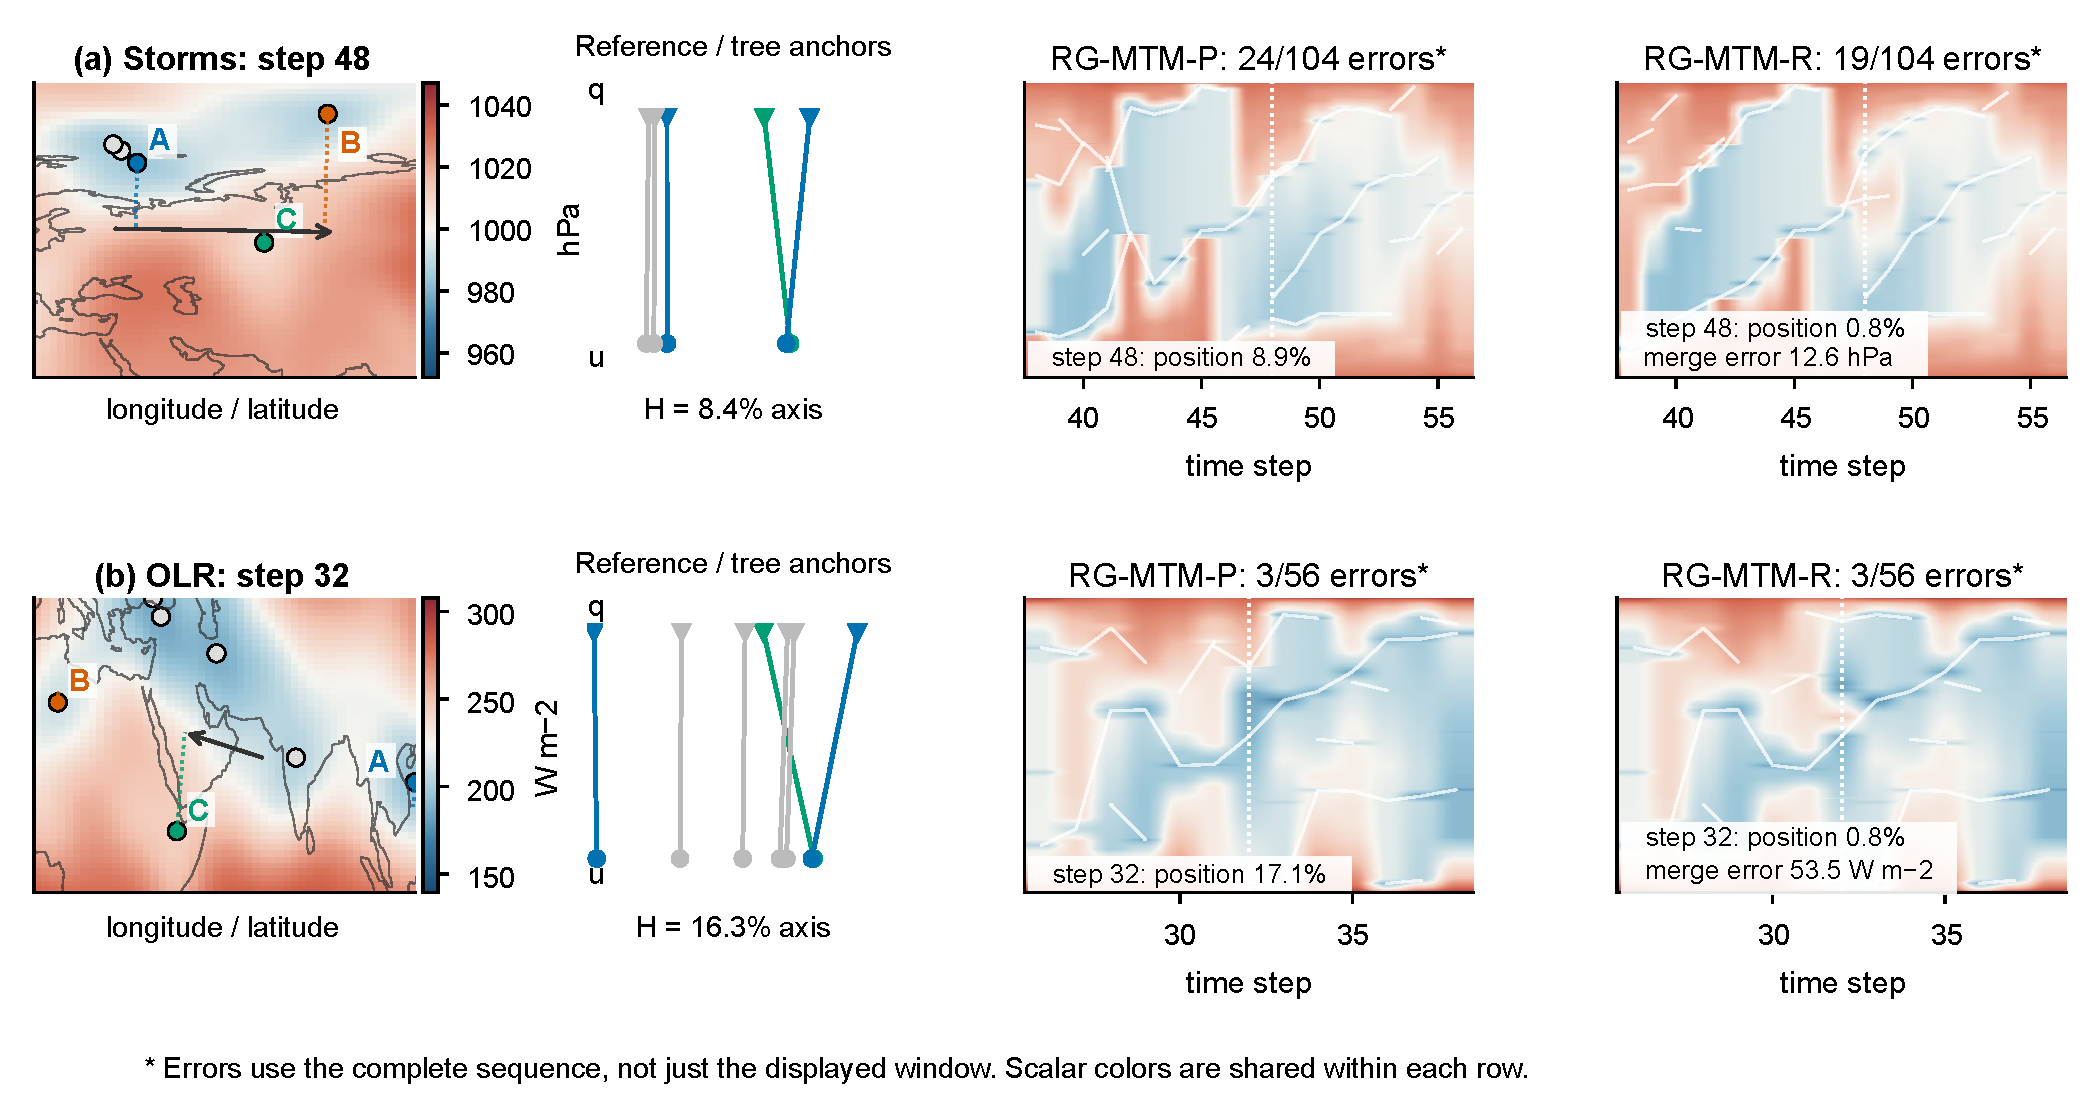
\includegraphics[width=\linewidth]{figures/rgmtm_linked_cases.pdf}
\caption{Local Storms and OLR witnesses retained from the previous integrated revision. Source fields, reference-to-anchor links, and P/R windows explain the individual hierarchy conflicts. Local labels report maximum anchor error and scalar cost; map titles give complete-sequence motion-proxy counts. Storms is the frame-48 example in the main introduction; OLR is the retained frame-32 example.}
\label{fig:s_local_witnesses}\end{figure}
The independent absolute-reference control is shown in main-paper Fig.~6. Section~\ref{sec:bisector_protocol} gives its protocol, calibration, and measurements; Fig.~\ref{fig:s_full_bisector_three_methods} retains the full visual comparison.
\clearpage
\subsection{Motion Errors and Scalar Costs}
\begin{figure}[H]\centering
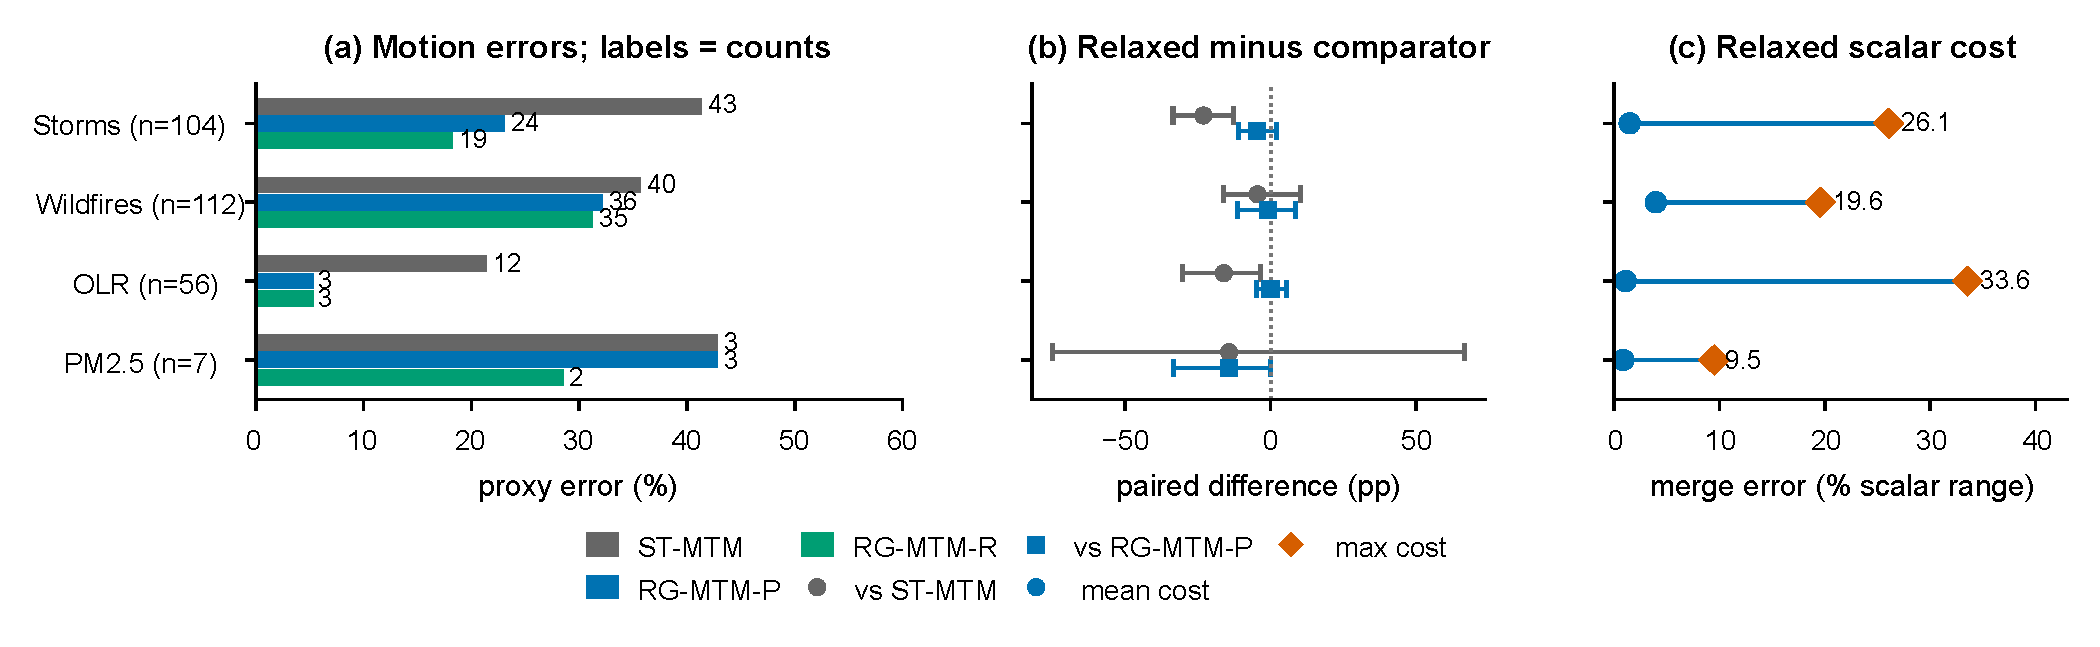
\includegraphics[width=\linewidth]{figures/rgmtm_motion_scalar_cost.pdf}
\caption{Four real sequences: primary motion-error counts and rates, paired relaxed-minus-comparator differences with retained temporal-block 95\% intervals, and relaxed mean/maximum scalar costs. The reference protocol fixes a two-step window and 2\% thresholds; PM2.5 has seven clear events. Scalar costs in this drawing use the saved fixed-order optimum; measured raster values agree to the numerical tolerance reported in the main text.}
\label{fig:s_motion_cost}\end{figure}
\begin{figure}[H]\centering
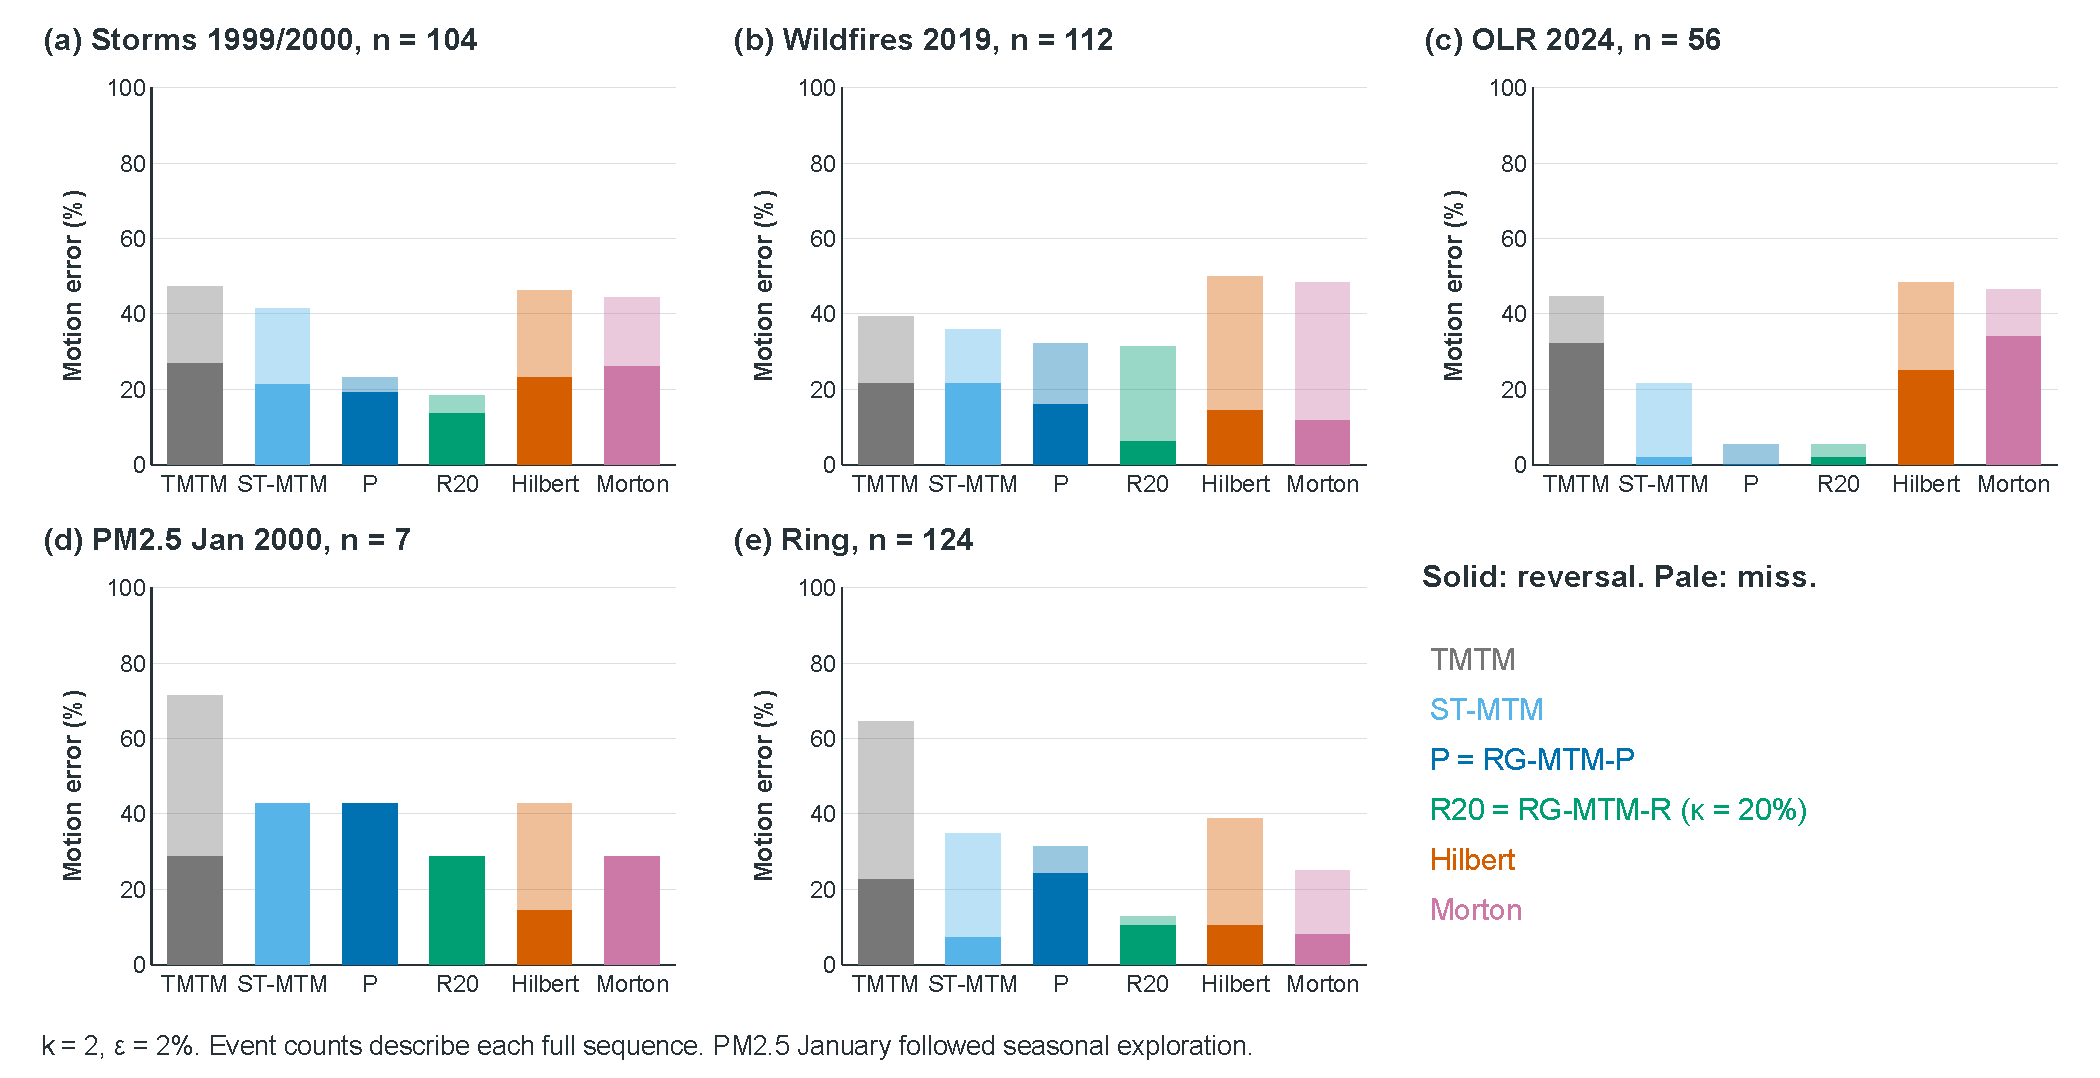
\includegraphics[width=\linewidth]{figures/rgmtm_motion_error_comparison.pdf}
\caption{Primary motion errors decomposed into reversals and misses across five sequences and the native curve controls. Solid portions show reversals and hatched portions show misses. Denominators are the shared clear two-dimensional events.}
\label{fig:s_motion_errors}\end{figure}

\subsection{Geometric Neighbourhoods}
\begin{figure}[H]\centering
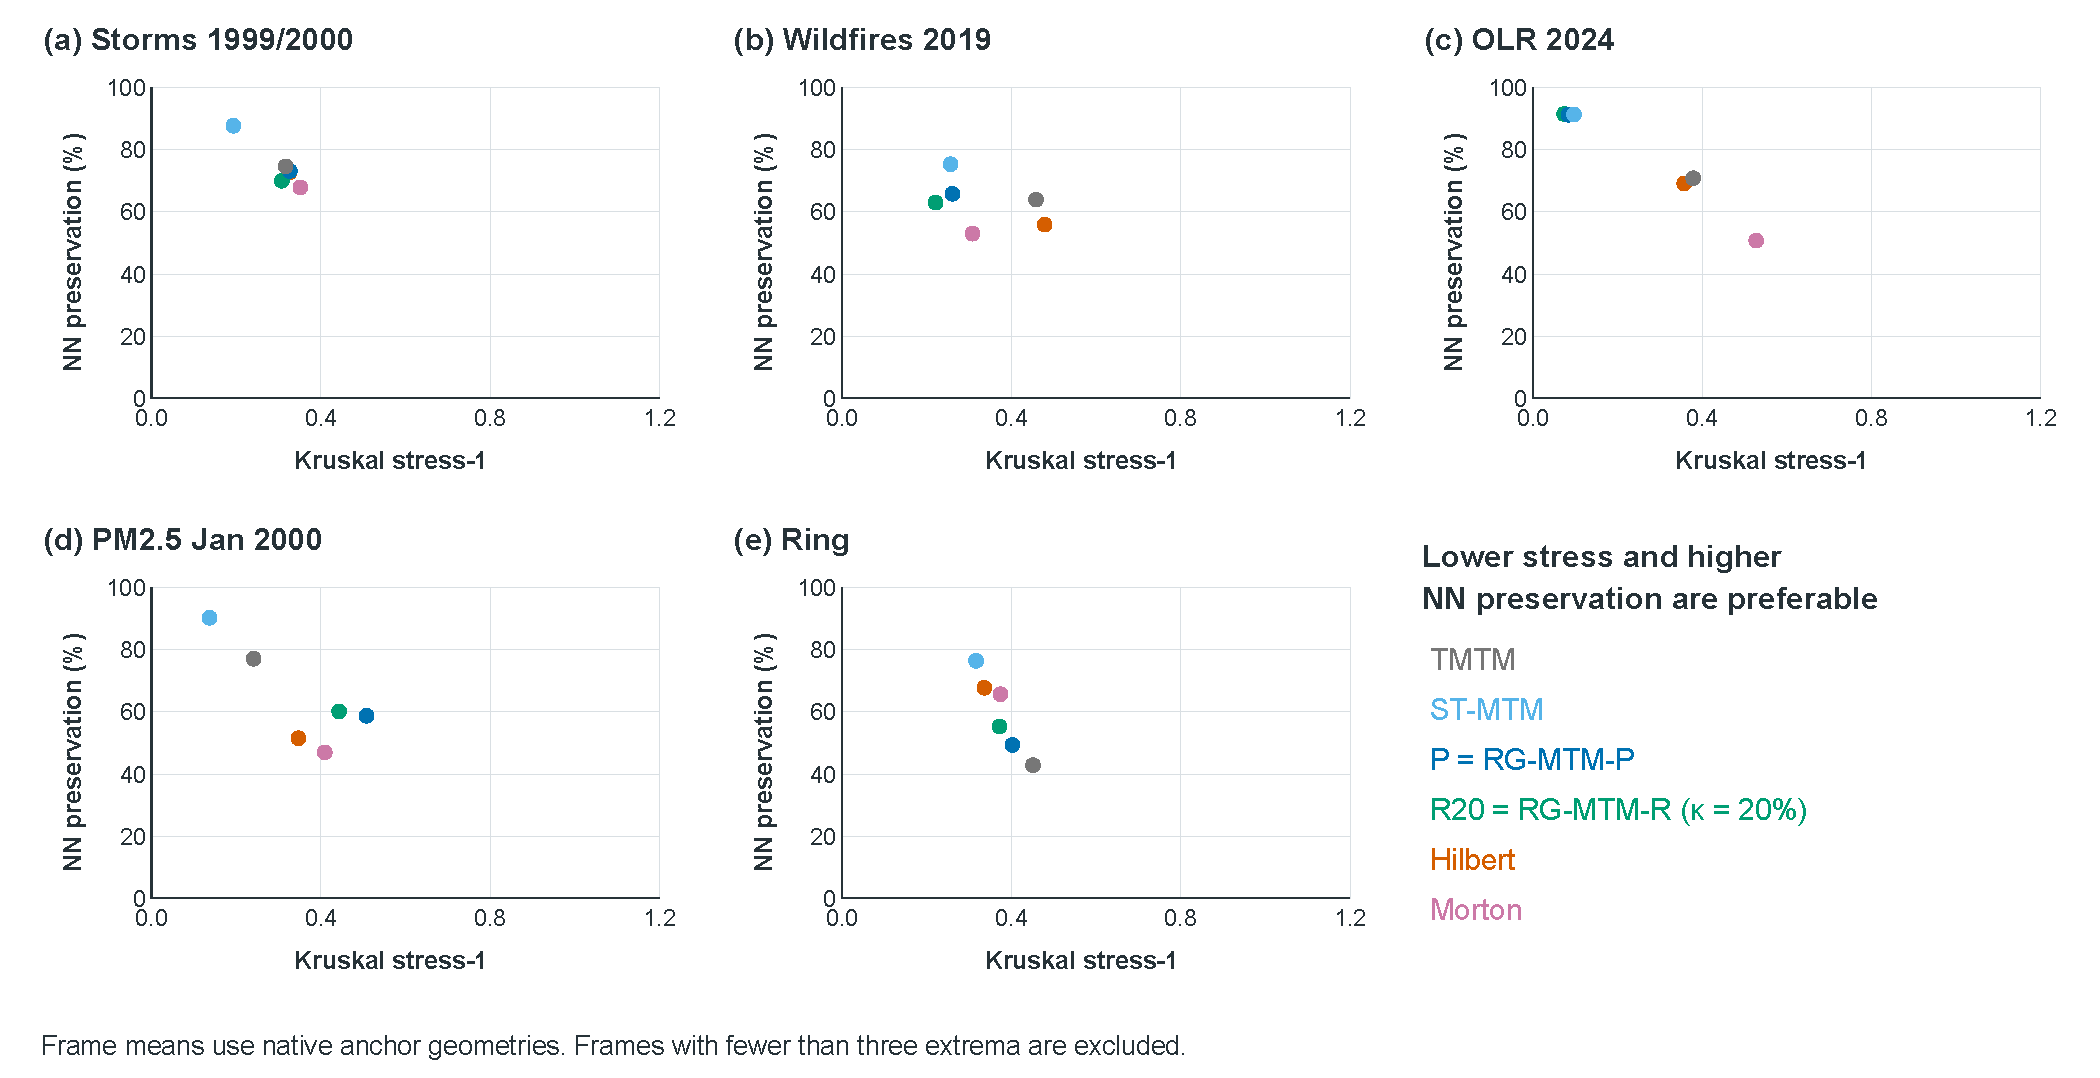
\includegraphics[width=\linewidth]{figures/rgmtm_neighbourhood_preservation.pdf}
\caption{Retained extremum-based stress-1 and nearest-neighbour identity preservation on frames with at least three extrema. Each method keeps its own anchor geometry. These metrics use different definitions from SNS and TW, whose complete values and eligible-frame counts are reported in Supplement S3.}
\label{fig:s_neighbours}\end{figure}

\subsection{Window Sensitivity}
\begin{figure}[H]\centering
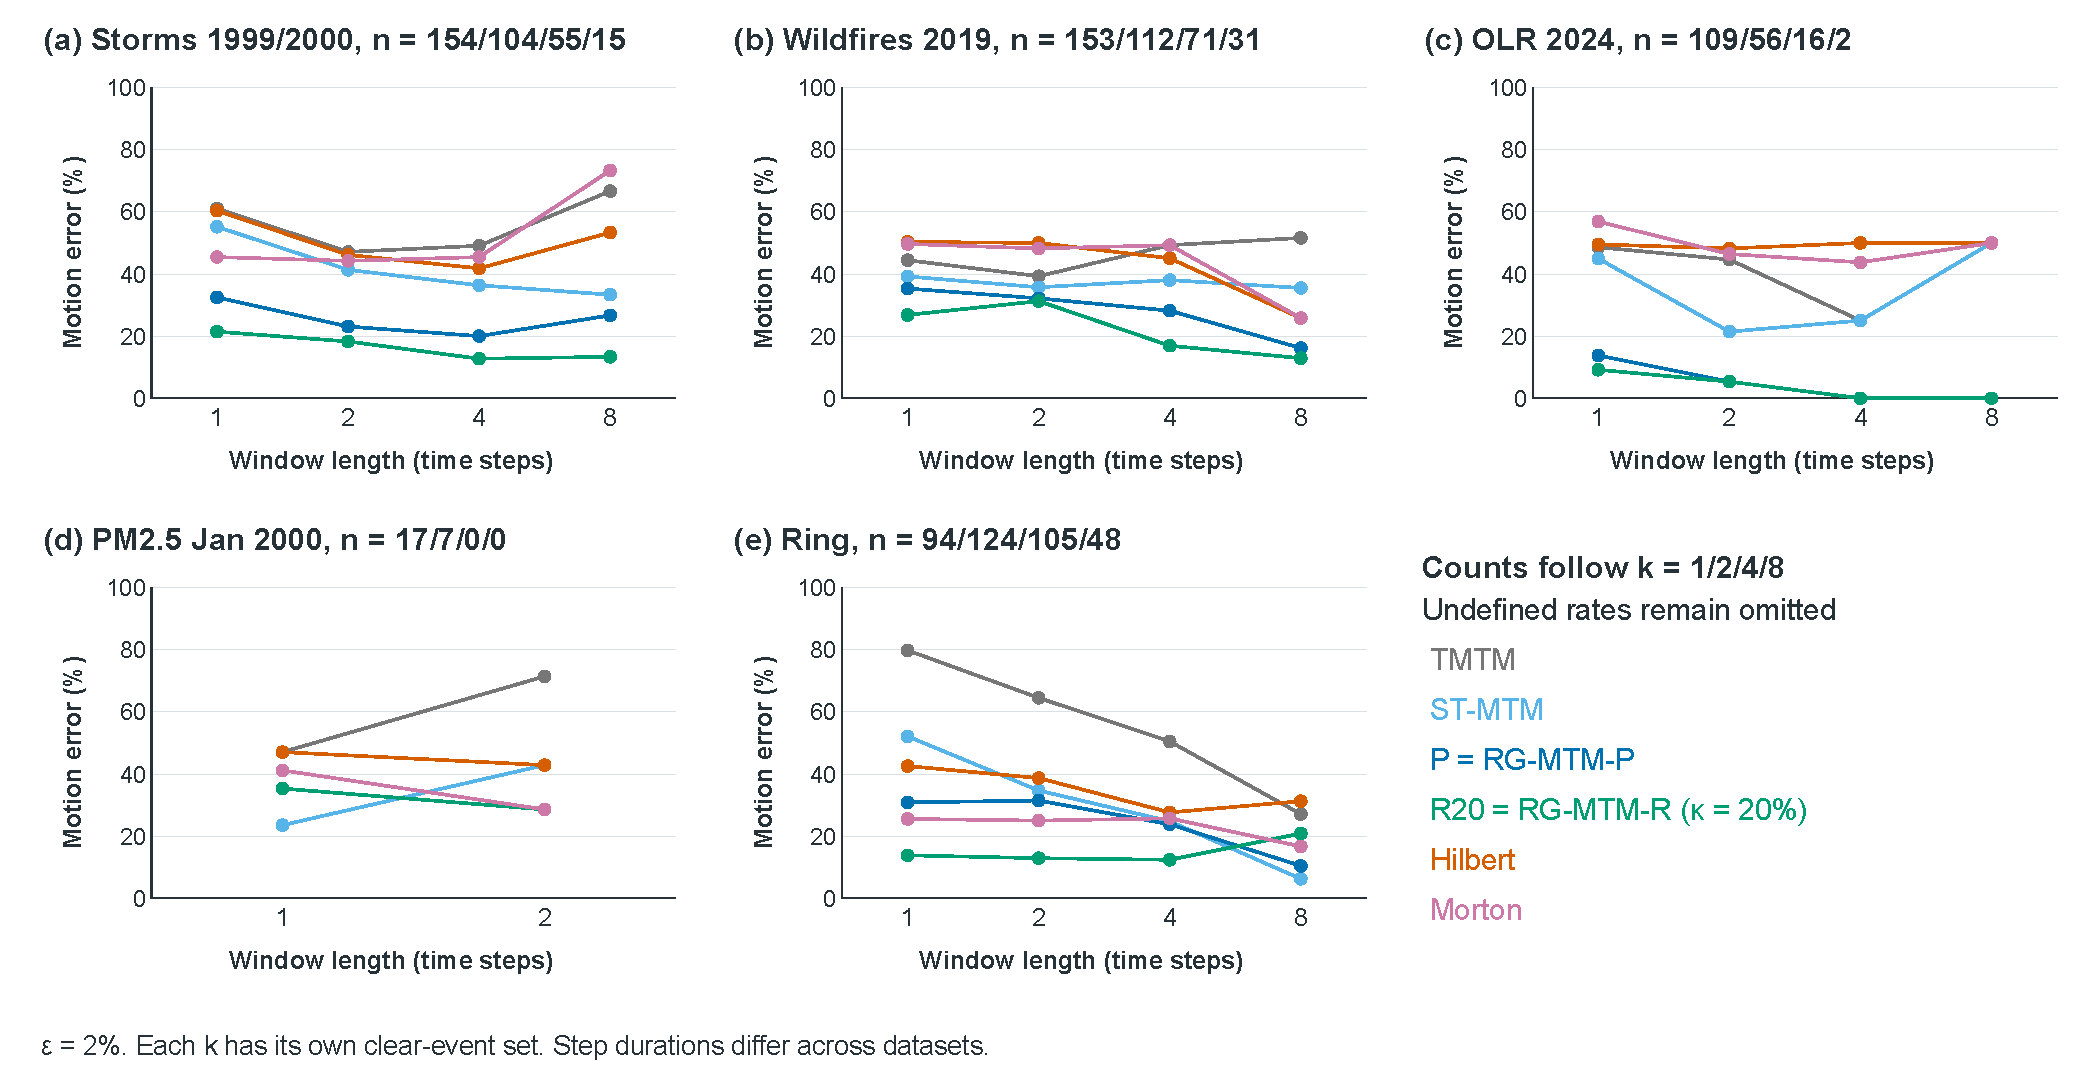
\includegraphics[width=\linewidth]{figures/rgmtm_motion_window_sensitivity.pdf}
\caption{Motion error for windows of 1, 2, 4, and 8 steps at the same 2\% thresholds. Each window has its own event set, with counts shown in that order above each panel. Sampling intervals differ by dataset. Undefined rates are omitted and their event counts remain explicit.}
\label{fig:s_windows}\end{figure}

\subsection{Native Sample Traversals and Scalar Cost}
\begin{figure}[H]\centering
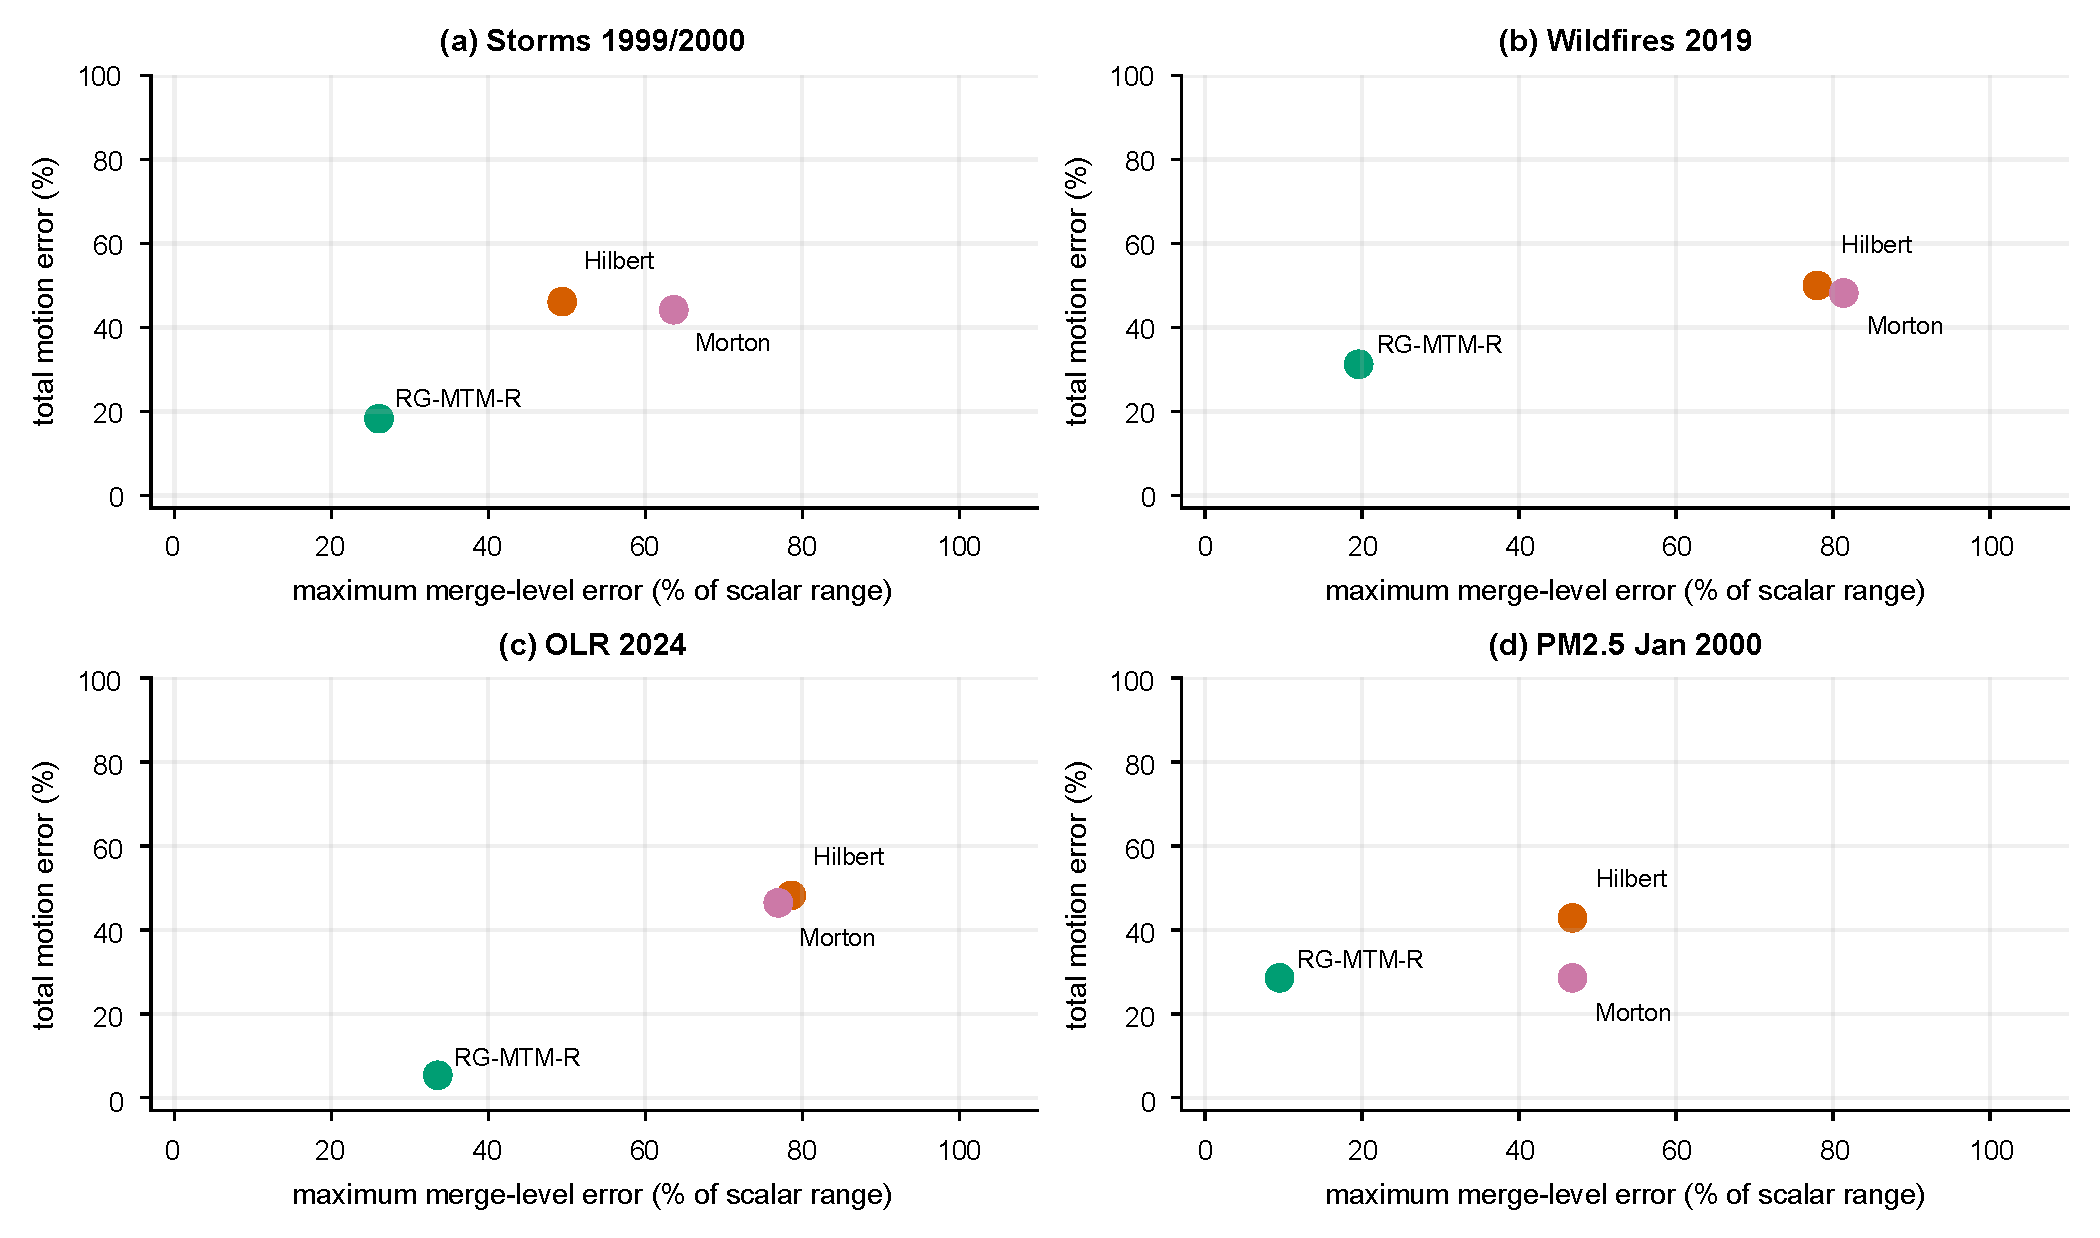
\includegraphics[width=\linewidth]{figures/rgmtm_topology_motion_tradeoff.pdf}
\caption{Motion error versus maximum merge-level distortion for RG-MTM-R and native Hilbert/Morton traversals. Each point is one fixed operating setting; native curves retain original sample values while RG-MTM-R uses optimal refilling. The comparison includes both ordering and rendering policy. Horizontal values are sequence maxima of the saved scalar-cost summaries.}
\label{fig:s_native_cost}\end{figure}

\clearpage
\section{Reproducibility and Evidence Roles}
The code repository contains experiment orchestration, method implementations, tests, and grouped numerical records; the local source package supplies this manuscript and supplement. The integrated source package contains the manuscript, supplement, selected existing figures, numerical evidence, and export documentation. Raw data are excluded and require the local prepared data or the acquisition steps in \path{data/README.md}. The independent runner invokes existing scientific entry points and records commands, runtime, exit status, source hashes, and result hashes. It does not change their algorithms or reported thresholds.

\paragraph{Main evaluation.} \path{experiments/publication2027/run.py} uses the five active sequences for the current submission and the five rerun numerical stages. Explicit selection of all ten available stages also recomputes replication, exact frontiers, direction robustness, persistence controls, and witnesses. Retained sensitivity records are not labelled new runs. Per-stage logs and completion manifests reside under \path{results/publication2027/runs/}.

\paragraph{Evidence packaging.} \path{experiments/publication2027/build.py} checks source hashes for positional and native-merge evidence, consistent frame counts, unique motion rows, and hierarchy lower bounds. It exports unrounded comparisons, a claim ledger, generated LaTeX tables, and source/snapshot hashes. The current submission snapshot in \path{results/submission20261023/} filters the five active small-tree sequences and adds the common-input static and volumetric summaries. The earlier five-sequence snapshot remains historical evidence and is not relabelled as a five-sequence run. Sensitivity, formal validation, protocols, and dendrogram transfer have separate folders. The original records remain available for historical traceability.

\paragraph{Numerical checks.} The existing test suite includes independent LP comparisons, grid lower-bound checks, projected-motion margins, native sample and barrier semantics, preprocessing contracts, and no-event handling. The historical implementation-validation run passed 43 tests; the current unified-model suite passes 57 tests; the separate standard-metric re-evaluation adds metric and reconstruction checks without method changes. The validation checks cover numerical optimization, rendering semantics, and metric reconstruction.

\paragraph{Publication configuration.} The main source uses the unmodified IEEE VGTC conference class in review mode. The main manuscript retains the supplied five-stage pipeline and integrates feature-linked Storms, Wildfires, and Tangaroa figures with the certificate and scalar-filling analysis. This supplement provides full derivations, pseudocode, protocols, complete geometric comparisons, and the volumetric evidence ledger. The additional mirror-motion control, static inputs, and volumetric sequences are reported separately from the five-sequence planar suite. Submission ID 0 is to be replaced with the PCS identifier; Codex assistance is disclosed in the acknowledgments.
\clearpage
\section{Original-Grid Tangaroa Protocol and Complete Evidence}
\subsection{Input processing and extracted features}
The formal volumetric entry point is \path{experiments/volume3d/run_paper.py}. The input contains all 201 official Tangaroa velocity fields, indices 0--200, time increment 0.01, on the original XYZ grid $300\times180\times120$. Physical bounds are $[-0.35,0.65]\times[-0.3,0.3]\times[-0.5,-0.3]$. Velocity magnitude uses float64 arithmetic followed by float32 storage. Values below $10^{-6}$ are replaced by 1; values are clipped to $[0,2]$. There is no spatial downsampling, Gaussian smoothing, per-frame normalization, or leaf-count-based frame selection.

TTK 0.9.9~\cite{Tierny:2018:TTK} traditional topological simplification modifies the scalar field at absolute persistence threshold 0.2, using regular-grid implicit triangulation, nonperiodic boundaries, no added scalar perturbation, and the returned symbolic offsets. The simplified field supplies the augmented join tree. This one persistence setting is fixed throughout the formal comparison. The actual trees contain 36--186 nodes and 18--93 leaves. TMTM reports 50--186 nodes for its 10\% row; the author-final scalar export and binary environment are unavailable, so exact derived-tree identity is unresolved. The public input grid and frame count agree, as do recorded magnitude fingerprints, including the initial raw maximum 3.0590057373046875.

Each leaf support contains its extremum vertex and incident leaf-arc regular samples. Its centroid and extremum position are computed in physical three-dimensional coordinates. Support volume equals sample count times the fixed physical sample measure. Positive original-voxel support intersections define a one-to-one Hungarian match. There are 6925 leaf-support instances, of which 2459 touch the boundary. The reference direction $(0.1019540600,-0.9945466284,-0.0219630047)$ uses 6214 matched extremum displacements and captures 0.5768552452 of their squared motion. The eight projected domain corners give origin $-0.3274590081$ and extent $L=0.7030746380$.

\subsection{Shared parameters and method-specific construction}
All rendered methods share the same TTK-simplified inputs and source merge targets. RG parameters are $c|\Omega|=L/2$, $g=L/240$, $\rho=0.5$, and allowance $\beta=L/120$. The hierarchy trigger is $H>0.02L$; eligibility fractions are 0.02, 0.2, and 1 of the declared scalar range 2. Volumetric R flattens every eligible non-root branching node and disables the optional two-dimensional restoration/pruning stage.

For continuous primary certificates, low-arity nodes use earliest-finish Pareto DP with bisection. Higher-arity cases use workload bounds or a 2-second HiGHS MILP, retaining feasible primal and dual bounds. With tree bounds $[l_T,u_T]$ and free-order bounds $[l_f,u_f]$, the hierarchy cost lies within $[\max(0,l_T-u_f),u_T-l_f]$. The gate activates when its lower bound exceeds $0.02L$, stays inactive when its upper bound does not, and preserves the hierarchy in unresolved cases. The formal run has 201 active, zero inactive, and zero unresolved original-tree gates.

Each layout uses the primary upper bound plus $\beta$. Candidate orders include the certificate witness, reference-preferred recursive order, previous-position-preferred recursive order, and TMTM order when legal and within budget. Duplicate candidates are removed; at most four are configured and at most three occur in the saved run. The convex QP records the constraint slack and the first-order gap from an independent linear oracle. This solves the secondary objective on the evaluated candidate set. Frames are processed sequentially.

TMTM starts at frame 100 and propagates top-down normal/reversed child decisions forward and backward using subtree overlaps. An $m$-way saddle requires $m-1$ separators: its source sample and $m-2$ additional copies at the same scalar value. Exactly 27 extra separators occur across the sequence. The source volume remains unchanged; saved sample IDs independently verify one occurrence of every original sample plus precisely those copies. The historical original-grid run did not include ST-MTM. The subsequent 201-frame ST-MTM extension now supplies a complete comparison in the main reference/motion and 3-D geometry tables; Supplement S3 gives its separately stored protocol, SNS/TW/TD and full-profile verification. Its scalar/path filler is also reused by RG. Separate synthetic three-dimensional extensions are retained outside this real-data table.

\subsection{Metric aggregation and complete parameter comparison}
NROE is the temporal mean of framewise width-free order error. Actual RG MAE averages rendered-anchor error within each frame and then over the 201 frames; this differs from the pooled continuous feature-frame displacement used for the planar suite. NMLE measures maximum pairwise source-LCA versus actual-profile merge discrepancy in each frame, divides by the declared scalar range 2, and reports temporal mean and maximum.

Motion compares labelled pairs shared by frames separated by lag 1, 2, or 4, with thresholds 1\%, 2\%, or 5\%. Spatial truth uses physical three-dimensional distance and domain diagonal; projected truth uses reference distance and $L$. Display decisions use the same fraction of each method's sequence-wide occupied anchor range. Default lag 2 and 2\% gives 6755 spatial clear events, including 1422 fully interior events, and 9631 projected clear events. These are different event sets. Table~\ref{tab:s_volume_complete} gives the default decomposition.

\begin{table}[H]\centering\small
\caption{Complete default Tangaroa measurements. Errors are percentages. Motion entries are reversal + miss counts; denominators are 6755 in 3D and 9631 for projected distance.}\label{tab:s_volume_complete}
\setlength{\tabcolsep}{4pt}
\begin{tabular}{lrrrrll}\toprule
Method & NROE & MAE & NMLE mean & NMLE max & 3D & Projected\\\midrule
TMTM & 20.09230 & -- & 0 & 0 & 185+6400 & 240+9168\\
P & 9.60801 & 5.12470 & 0 & 0 & 1613+2084 & 2072+2973\\
R2 & 8.56031 & 4.31072 & 3.51512 & 11.53659 & 1467+1811 & 1601+2322\\
R20 & 0.018945 & 1.06487 & 14.44212 & 31.02051 & 826+1234 & 22+218\\
R100 & 0.018945 & 1.06487 & 14.44212 & 31.02051 & 826+1234 & 22+218\\
Exact projection & 0 & 0 & -- & -- & 763+1297 & 0+0\\
\bottomrule\end{tabular}
\end{table}

P and TMTM have zero measured source-leaf merge error in all 201 frames; R2 has three zero-error frames and R20/R100 have none at tolerance $10^{-6}$. The primary P certificate has maximum bracket width $1.98358\times10^{-10}L$. R2 has 48 brackets not closed to tolerance and maximum width $0.0956105L$; R20/R100 close to tolerance in this sequence. The maximum selected-QP first-order gap, normalized by $L^2$, is $2.03871\times10^{-7}$; over all evaluated candidates it is approximately $2.06326\times10^{-7}$. Maximum anchor-rounding and interval-width errors are $3.81427\times10^{-6}L$ and $7.61058\times10^{-6}L$.

\subsection{Independent verification and display provenance}
The retained full numerical verification independently re-read 201 original velocity volumes, checked ZIP CRC32 and SHA256, reconstructed all 1,302,480,000 preprocessed scalar samples, and obtained zero maximum difference. It verified augmented sample ownership, arc monotonicity, physical extrema and centroids, support measures, direct parent-chain LCA targets, every full saved map's measured barriers, layout budgets, interval constraints, and TMTM sample-ID multiplicities. A separate rounded-down grid check provided continuous-certificate lower bounds at eleven uniformly spaced frames. These results are stored in \path{results/volume3d/tangaroa-paper-p10-full201/verification.json}.

\path{metrics.json} stores all motion settings; \path{frame_metrics.json} stores complete per-frame measurements, layouts, bounds, and array hashes; \path{protocol.json}, \path{manifest.json}, \path{features.json}, \path{reference.json}, and \path{certificates.json} bind the inputs, source code, and numerical results. Full source volumes, simplified scalars, and 131072-row RG maps remain in local prepared-data storage. The lightweight \path{verify_saved.py} checks distributed evidence bindings, whereas \path{verify_paper.py} performs full numerical verification with the local arrays.

Main-paper Figure~15 and the complete comparison in S10 reuse frozen 4096-row display samples for all 201 frames, with a local window at 135--145 and source-volume views at 139--141. The source views show pre-TTK near-zero-replaced and clipped magnitudes; simplified-input renderings and earlier context views at 0, 100, and 200 remain separately archived. The main views share the original purple--white--orange transfer function and one full-domain orthographic camera; S8 records the camera and projected-marker provenance. These display choices do not change the trees, layouts, or metrics, which use the full arrays. R100 duplicates R20 in this formal comparison, while input persistence remains fixed at 10\%.

\begin{table}[t]
\caption{Detailed volumetric settings under the same shared metric definitions (percent and errors/clear events).}\label{tab:volume}
\centering\footnotesize\setlength{\tabcolsep}{4pt}
\resizebox{\linewidth}{!}{\begin{tabular}{llrrrrll}\toprule
Data & Method & NROE & $E_{\rm pool}$ & NMLE mean & NMLE max & Spatial motion & Projected motion\\\midrule
Tangaroa & TMTM & 20.092 & n/a & 0.000 & 0.000 & 6585/6755 & 9408/9631\\
Tangaroa & RG-MTM-P & 9.608 & 5.013 & 0.000 & 0.000 & 3697/6755 & 5045/9631\\
Tangaroa & R, $\kappa=2\%$ & 8.560 & 4.165 & 3.515 & 11.537 & 3278/6755 & 3923/9631\\
Tangaroa & R, $\kappa=20\%$ & 0.019 & 1.176 & 14.442 & 31.021 & 2060/6755 & 240/9631\\
Tangaroa & R, $\kappa=100\%$ & 0.019 & 1.176 & 14.442 & 31.021 & 2060/6755 & 240/9631\\
Tangaroa & Exact projection & 0 & 0 & n/a & n/a & 2060/6755 & 0/9631\\
Cylinder & TMTM & 26.617 & n/a & 0.000 & 0.000 & 2141/3196 & 1845/2934\\
Cylinder & RG-MTM-P & 12.262 & 5.400 & 0.000 & 0.000 & 1191/3196 & 870/2934\\
Cylinder & R, $\kappa=2\%$ & 0.249 & 0.623 & 0.692 & 4.886 & 617/3196 & 123/2934\\
Cylinder & R, $\kappa=20\%$ & 0.084 & 0.550 & 2.810 & 14.281 & 605/3196 & 108/2934\\
Cylinder & R, $\kappa=100\%$ & 0.084 & 0.550 & 3.190 & 14.281 & 606/3196 & 107/2934\\
Cylinder & Exact projection & 0 & 0 & n/a & n/a & 603/3196 & 0/2934\\
\bottomrule\end{tabular}}
\par\smallskip{\footnotesize\raggedright The main paper common result tables include these inputs; this supplementary table expands only the parameter and projection checks. $E_{\rm pool}$ uses continuous, pooled anchors. Spatial and projected motion have their own denominators and cannot be subtracted as a causal decomposition. Optional strongest-first hierarchy pruning is disabled for these larger inputs; $\kappa$ is not a measured scalar cap. This historical parameter table retains its original configurations; the completed ST-MTM comparison and all-method geometry results are in S3 and the current main tables.\par}
\end{table}


\clearpage
\section{Event Correspondence and Baseline Audit}\label{sec:event_audit}
\subsection{Frozen case figures and selection}
The event-linked drawings use the existing arrays in \path{results/real_case_studies/evidence/}: retained scalar profiles, extremum coordinates, overlap matches, and original-observation or original-grid volume views. The three-page \path{rgmtm_large_figures.pdf} and its individual vector pages are preserved in \path{figures/source/real_case_studies/}. The preceding P/R-only panels remain as traceable sources. The main paper shows source-linked P/R maps; S10 retains saved TMTM/ST-MTM planar profiles and saved TMTM volumetric profiles, using their native ordinates alongside the RG reference axis. Complete-frame maps retain all time steps; local enlargements state their own coordinate ranges. Source markers and temporal anchors use recorded transformations (S8). The plotting export calls no extraction, layout solver, metric evaluation, or volume renderer.

Storms frame 48 is the previously retained interior hierarchy witness. W1 selects the largest hierarchy cost, with earliest-frame tie-breaking, among above-trigger Wildfires frames having a three-frame matched conflict triple and positive displacement reduction and scalar cost. These choices explain individual constructions; the complete-sequence tables provide the performance evidence. The archived Storms storm-time guides and Tangaroa context views follow the reference papers' selected temporal contexts independently of these witness-selection rules. Current main figures instead use the hourly Storms visualization and the Tangaroa frame-140 conflict window; their distinct populations and coordinates are documented in S8.

\subsection{Storms storm-time correspondence}
TMTM Fig.~1~\cite{Koepp:2023:TMTM} supplies five December 1999 times; ST-MTM Fig.~6~\cite{STMTM:2026} discusses the same month's storms. Convert an elapsed time from 17 November 1999 00 UTC into frame index by dividing by 12 hours. Table~\ref{tab:s_era_event_times} separates each fractional guide position from the discrete snapshot. The circles locate nearby computed pressure minima, identified by the stored overlap-track IDs. Event labels specify temporal correspondence, not independently validated cyclone identity. E4 carries a time guide and a source snapshot without an assigned named-storm leaf.

\begin{table}[H]\centering\small
\caption{Reference-paper storm times and local Storms snapshots. Dates are in December 1999, UTC; fractional indices locate the dashed guides.}\label{tab:s_era_event_times}
\setlength{\tabcolsep}{5pt}
\begin{tabular}{llrrrr}\toprule
Guide & Reference-paper context & Day/time & Index & Snapshot & Track\\\midrule
E1 & Anatol & 03 / 18:00 & 33.500 & 34 & 37\\
E2 & Scandinavia storm & 17 / 21:00 & 61.750 & 62 & 66\\
E3 & British Isles/Norway storm & 24 / 23:00 & 75.917 & 76 & 87\\
E4 & Lothar time window & 26 / 10:00 & 78.833 & 79 & --\\
E5 & Martin time window & 27 / 21:00 & 81.750 & 82 & 93\\
\bottomrule\end{tabular}\end{table}

The reference papers use 744 hourly pressure-anomaly fields. The quantitative sequence audited here instead uses 118 half-day MSLP fields, a different region, and 250-km smoothing/minimum extraction. The main-paper teaser is a separate 744-hour anomaly visualization with its own extrema and track identifiers. Storms frame 79 contains two retained leaves and no independently identified Lothar leaf. These input differences determine what can be matched beyond a calendar time. Track 66 at frame 62 has normalized reference 0.637427, P anchor 0.600655, and R anchor 0.648027; the plotted markers use these saved coordinates.

\subsection{Wildfires witness, scalar values, and temporal links}
W1 is frame 18, the two-day FRP aggregate starting 7 December 2019. The source snapshots show unsmoothed log-transformed observations; the circles are extrema of the processed split-tree field. Tracks $A,B,C$ are IDs 3, 48, and 52, corresponding to local leaves 3192, 419, and 3285 at W1. Their preceding positive support-overlap IoUs are 0.306, 0.893, and 0.746, and all three continue to the next frame. The reference order is $A,C,B$; the original subtree joins $A,B$ before the outside leaf $C$.

\begin{table}[H]\centering\small
\caption{Saved normalized reference and anchor coordinates of the W1 triple at frame 18. These use the complete shared reference extent.}\label{tab:s_fire_positions}
\begin{tabular}{lrrrrr}\toprule
Feature & Track & Reference & P anchor & R anchor & Extremum value\\\midrule
A & 3 & 0.169078 & 0.193307 & 0.166133 & 2.408155\\
B & 48 & 0.684591 & 0.537046 & 0.704579 & 0.765362\\
C & 52 & 0.418239 & 0.549117 & 0.421862 & 0.193260\\
\bottomrule\end{tabular}\end{table}

The original split-tree connection levels for $AB$, $AC$, and $BC$ are 0.060800, 0.003617, and 0.003617. P retains them. The measured relaxed levels are $-0.574262$, 0.001144, and $-0.574262$, giving analytical fixed-order error 0.635062. The saved profile has measured worst-pair error 0.635063 after strict-extremum clearance, or 15.0944\% of the processed sequence range (S8). Negative output levels are artificial connection values introduced by the fixed-extremum minimax correction; they are not negative FRP observations and are shown with an explicit blue under-range colour. The local scalar range and the theoretical fixed-order cost remain distinct from this measured output discrepancy. No physical fire-entity identification is inferred from the computational track IDs.

\subsection{Tangaroa temporal context and display provenance}
The T1--T3 indices 25, 100, and 145 correspond to source times 0.25, 1.00, and 1.45 in the original 201-frame sequence. They follow TMTM Fig.~15 and its Tangaroa discussion: approximately frame 25 for reported group separation, frame 100 for the two-group volume illustration, and approximately frame 145 for a departing group's disappearance. TMTM Fig.~14 instead concerns Cylinder; its phase labels are not transferred to Tangaroa. ST-MTM provides no corresponding real three-dimensional experiment.

These are temporal context links, not verified cross-method feature-group identities. The RG axis is a fixed directional projection and differs from the original TMTM linearization coordinate. Source-volume snapshots at 0, 25, 100, 145, and 200 reuse \path{tangaroa_event_volumes.npz}; the views at 25 and 145 were added in the preceding case-study task, and all five were already cached before manuscript integration. They show pre-TTK near-zero-replaced and clipped magnitudes; the time maps retain the fixed-10\%-persistence join-tree inputs specified in S6. These archived context views are distinct from the current main-paper views at frames 139--141, whose camera and marker provenance are documented in S8.

\subsection{Baseline algorithm checks on 148 real-data frames}
The existing audit covers 118 Storms frames and 30 Wildfires frames. TMTM is checked against the official repository at \url{https://github.com/Wiebke/TemporalMergeTreeMaps}. The fixed revision is recorded separately:
\begin{quote}\small\texttt{2c75a10ed2cd55177a25ff751e0c0a8261200717}\end{quote}
A harness compiles the author's \texttt{LandscapeInfo}, \texttt{objectiveForSeveralArcs}, \texttt{decideGreedy}, and \texttt{decideGreedyTree} core, supplying the same extracted real trees and spatial overlap counts. Every one of 486 branch decisions and 1118 interval/anchor records agrees. All processed samples appear once, subtree leaves remain contiguous, and measured pairwise merge error is zero in all 148 frames. This verifies the tested binary core, separately from a complete author Inviwo/TTK environment.

ST-MTM checks reconstruct the distance/temporal objective and relative-width objective independently in matrix form, with feasibility and nonnegative-multiplier KKT stationarity checks. The audit also checks concordance, threshold/orientation logic, and all four filling-path cases. The 148 rendered profiles retain zero pairwise merge-level error and have no failed complete topology signatures. Table~\ref{tab:s_baseline_audit} reports the primary-setting residuals; they are optimizer residuals, not layout-quality scores.

\begin{table}[H]\centering\small
\caption{Independent baseline audit. ST entries are maximum relative KKT residuals for the paper's first and second optimization problems under the current shared-input settings.}\label{tab:s_baseline_audit}
\begin{tabular}{lrrrrrr}\toprule
Data & Frames & TMTM decisions & Intervals/anchors & ST Eq.1 & ST Eq.2 & OLO gaps\\\midrule
Storms & 118 & 285 & 687 & $3.55\times10^{-8}$ & $1.25\times10^{-8}$ & 1\\
Wildfires & 30 & 201 & 431 & $1.89\times10^{-8}$ & $9.63\times10^{-7}$ & 7\\
\bottomrule\end{tabular}\end{table}

\paragraph{Ordering heuristic.} ST-MTM's stated SciPy OLO step is retained as a heuristic. With SciPy 1.13.1, independent exhaustive legal-order checks find larger adjacency costs in eight frames (Table~\ref{tab:s_olo_gaps}); the implementation is not silently replaced by an exhaustive sorter. Subsequent temporal orientation and quadratic optimization follow their declared protocol. Author-code equivalence is not claimed for ST-MTM: the available preprint states that its complete implementation will be released after acceptance.

\begin{table}[H]\centering\small
\caption{All audited frames where the SciPy OLO adjacency cost exceeds the exhaustive legal-order minimum. Costs use the corresponding input-coordinate distance units.}\label{tab:s_olo_gaps}
\begin{tabular}{lrrr}\toprule
Data & Frame & SciPy cost & Exhaustive minimum\\\midrule
Storms & 24 & 182.717226 & 152.485568\\
Wildfires & 0 & 134.960780 & 127.765618\\
Wildfires & 1 & 185.488174 & 149.395419\\
Wildfires & 3 & 211.222797 & 209.969161\\
Wildfires & 8 & 302.781490 & 251.500432\\
Wildfires & 10 & 256.211632 & 256.089992\\
Wildfires & 11 & 254.944394 & 242.866054\\
Wildfires & 17 & 226.294598 & 221.158409\\
\bottomrule\end{tabular}\end{table}

\paragraph{Shared-input settings and original-paper settings.} The main comparison uses an ST-MTM reimplementation under the shared-input protocol. Its dataset configuration differs from the original paper's configuration (Table~\ref{tab:s_baseline_parameters}). $K$ has input-coordinate length units; frame counts, scalar preprocessing, and tree inputs also differ. The audit checks equations and constraints without substituting original-paper parameters or changing any reported result.

\begin{table}[H]\centering\small
\caption{Current ST-MTM comparison settings and reference-paper settings. $N$ is layout raster length; $\lambda$ is temporal weight.}\label{tab:s_baseline_parameters}
\setlength{\tabcolsep}{5pt}
\begin{tabular}{lllrrrrr}\toprule
Data & Protocol & Weights & $K$ & $r$ & $\lambda$ & $N$ & Start\\\midrule
Storms & Current & uniform & 5.644221 & 0.95 & 0.5 & 4096 & 0\\
Storms & Reference & inverse & 135 & 0.65 & 0.05 & 4096 & 40\\
Wildfires & Current & uniform & 6.269531 & 0.95 & 0.5 & 2048 & 0\\
Wildfires & Reference & uniform & 10 & 0.85 & 0.5 & 4096 & 5\\
\bottomrule\end{tabular}\end{table}

\paragraph{Tangaroa provenance.} The audit rechecks the bindings of the saved 201-frame independent verification. Four generic Tangaroa preset entries were corrected from split to join trees; the active original-grid 201-frame pipeline already used join trees and its saved results are unchanged. The same-value multiway-saddle separators disclosed in S6 remain a declared extension of the original binary-tree TMTM core. The 36--186 derived-node range and the absence of a completed real-3D ST-MTM layout run retain the scope stated in S6.

\paragraph{Evidence preservation.} The audit's \path{validation.json} reports 177 protected numerical files unchanged. No scientific stage is rerun for this manuscript revision. The paper package includes the existing audit JSON, preset-correction record, event-correspondence JSON, per-case event evidence, and figure hashes in \path{evidence/event_case_revision/} and \path{figures/source/real_case_studies/}. The full local sources remain \path{results/baseline_audit_20261019/} and \path{results/real_case_studies/}; the manuscript's publication-size figure export records its frozen-input hashes separately.

\clearpage
\section{Revised Figure Evidence and Coordinate Semantics}\label{sec:revision_figures}
\subsection{Hourly Storms teaser: selected window and eligibility sweep}\label{sec:s_hourly_teaser}
Main-paper Figure~1 uses the separate December 1999 hourly pressure-anomaly experiment, not the 118-frame half-day evaluation. The saved full-month R20 overview contains 744 original hours. Its orange box selects frames 30--46 (2 December, 06:00--22:00 UTC; 17 profiles) and normalized output positions $[0.10,0.42]$. The selected original scalar columns are identical to the corresponding R5 columns. Source snapshots are frames 33, 34, 35, 37 and 42 (09:00, 10:00, 11:00, 13:00 and 18:00). They show supplied-grid anomalies with the same centered 192-hour baseline; marker coordinates belong to the retained $49\times49$, 250-km-smoothed analysis. The full-month direction and canvas remain fixed throughout the sweep.

The local conditions use the retained construction. P preserves the hierarchy; R1, R2 and R5 use eligibility fractions $\kappa/\Delta_F=0.01$, $0.02$ and $0.05$, respectively. This fraction restricts merge relaxations and does not bound the measured output error. Each condition is solved forward from the original frame 0 through frame 96, retaining its own incoming temporal history; the selected window is not reset or assigned a newly fitted direction. The recomputed R20 prefix reproduces the saved full-month scalar columns exactly, with maximum anchor discrepancy $2.22\times10^{-16}L$. These additional illustrative layouts do not change the 614-frame or 325-input evaluation populations.

Letters $A,B,C,D,E,F$ identify computational tracks 7, 5, 8, 9, 10 and 0. At 09:00, $A$ is at $20.714^\circ$W, $31.586^\circ$N and $B$ at $15.000^\circ$W, $66.012^\circ$N. At 13:00, $A$ is at $22.143^\circ$W, $32.227^\circ$N and $C$ at $12.143^\circ$W, $66.012^\circ$N. At 18:00, $D$, $E$ and $F$ are at $(23.571^\circ\mathrm{W},32.874^\circ\mathrm{N})$, $(22.143^\circ\mathrm{W},53.085^\circ\mathrm{N})$ and $(12.143^\circ\mathrm{W},64.705^\circ\mathrm{N})$. Track 10 is the computed minimum associated with the Anatol context. Positive-overlap matching supplies these labels without independently verifying meteorological identity. $B$ ceases to be an independent tracked extremum after 09:00; $C$ receives a new identifier at 12:00. Geographic proximity does not establish a physical B--C identity. Only feature/hour pairs present in the five displayed snapshots receive markers; the scientific profiles retain all hourly values.

The directional-order examples are checked on saved references and anchors: R5 restores $A/B$ at 09:00, R1 restores $A/C$ at 13:00, and R2 restores $E/F$ at 18:00. The unchanged position of $A$ at 09:00 and 10:00 gives a separate layout-motion example: both references are $0.339258L$, but the P anchors are $0.237936L$ and $0.347592L$; R5 uses $0.347592L$ at both hours. Thus the illustrated jump is not a geographic displacement.

\begin{table}[H]\centering\small
\caption{Direct measurements for the 17-hour selected window, over all retained extrema and all leaf pairs in the full profiles. These values are illustrative window summaries, not additions to the main evaluation.}
\begin{tabular}{lrrr}\toprule
Condition & Mean position error (\%$L$) & Max position error (\%$L$) & Max merge error (hPa)\\\midrule
P & 2.3765 & 10.1323 & 0\\
R1 & 2.0710 & 10.1323 & 0.2580\\
R2 & 1.6700 & 10.1323 & 0.4260\\
R5 & 0.8996 & 2.5427 & 1.1549\\\bottomrule
\end{tabular}\label{tab:s_hourly_teaser}
\end{table}

All panels share the $[-35,35]$\,hPa display scale. Conservative anchor-aligned reconstruction preserves every original 4096-row hourly column, falling back to fixed-position interpolation across unsupported order changes or large jumps. Intermediate columns are display samples, not observations. Original coordinates, arrays, direct merge measurements, display checks and editable figure sources are frozen in \path{evidence/storms_teaser20261026/}.

\subsection{Source identities and selected frames}
The feature-linked figures read frozen arrays in \path{results/real_case_studies/evidence/}. No feature extraction, layout construction, persistence change, or experiment is rerun. Storms frame 48 is the previously retained witness. Wildfires frame 18 maximizes hierarchy cost among above-trigger frames with a persistent three-frame triple and positive position gain and scalar cost, with earliest ties. Tangaroa frame 140 maximizes achieved P-to-R displacement reduction among above-trigger frames with a persistent triple and positive scalar cost. These descriptive selection rules emphasize visible mechanisms; all performance summaries remain the complete-sequence results.

The underlying rows identify extrema by retained leaf IDs and positive-overlap track IDs. A track born within the enlarged window begins there; no trace is extrapolated to an absent feature. All scalar values, anchor coordinates, and error summaries come from saved records. Markers use the processed-field extrema over the raw source observations or pre-TTK volume views.

\begin{table}[H]\centering\small
\caption{Selected-frame evidence. Position quantities are percentages of fixed reference extent; NMLE is percentage of the processed sequence range. Tangaroa $H$ is a lower bound. These rows are separate cases, not a pooled mean.}
\begin{tabular}{lrrrrrr}\toprule
Case/frame & Leaves & Packing & $H$ & Max P & Max R20 & Actual NMLE\\\midrule
Storms/48 & 5 & 0 & 8.4484 & 8.8665 & 0.8333 & 13.2079\\
Wildfires/18 & 10 & 0 & 13.9211 & 14.7545 & 2.6328 & 15.0944\\
Tangaroa/140 & 27 & 0.1827 & $\ge13.7442$ & 14.7605 & 1.0164 & 13.7502\\\bottomrule\end{tabular}
\end{table}

\paragraph{Analytical cost and rendered measurement.} The planar event JSON fields named \path{actual_max_merge_error} were populated from the filling routine's returned analytical $\delta^*$, before the positive strict-extremum clearance. Direct all-pair checks on the saved complete columns give Storms frame 48: analytical 12.557166\,hPa, measured 12.558173\,hPa (13.207872\% NMLE); Wildfires frame 18: analytical 0.635061777, measured 0.635062968 (15.094425\% NMLE). The revised frame-level text and captions use the measurements. The original JSON and all 177 protected result files remain unchanged; the correction is documented in the revision checks. Sequence-level main tables already use the independently measured filling records.

\subsection{Coordinate transformations and display resolution}
A temporal panel covering frames $l,\ldots,r-1$ maps frame $t$ to $x=x_0+(t-l+1/2)w/(r-l)$. Its vertical mapping is $y=y_0+(b-v)h/(b-a)$ for the displayed ordinate range $[a,b]$. Complete maps use $[0,1]$; local windows explicitly label cropped ranges. TMTM and ST-MTM normalize their own native sample domains to this unit interval. Only RG maps identify that interval with the fixed directional reference. Dashed reference tracks appear only in RG panels.

The scalar images are nearest-neighbour displays of the frozen profiles. Tangaroa's cached 4096-row display may omit narrow extrema at nearby rows. Exact full-resolution anchors are therefore overlaid independently from the retained positions; they are not snapped to the preview colours. All Tangaroa metrics use the 131072-row outputs, not these previews.

Storms source layers use the existing geographic transformation and coastline, with each extremum transformed from its processed-grid position. Wildfires source layers retain the full $[0,120]^2$ domain, unsmoothed raw log-FRP observations, and the saved processed extrema. Main-paper Figure~9 uses a light yellow--orange--brown palette with unchanged linear normalization: processed maps use $[0,4.207268783]$ and raw snapshots use $[0,12.050886763]$. Artificial negative connection values use grey-blue. The five main-paper raw snapshots have equal domain scale, and track labels terminate at the last saved sample. The original three-frame comparison remains in S10. Additional source-view records are in \path{evidence/dimensional_results/source_views.json}. Palette and coordinate records are retained in \path{evidence/figure8_display/}. Three Tangaroa images come from \path{tangaroa_volumes.npz}, frames 139, 140, and 141. For the framed views in main-paper Figure~15, the same original-grid scalar frames are rendered with the original transfer function and an orthographic display camera yawed by $18^\circ$ from the preceding view. One affine projection maps the volume, all eight domain corners, and the marked three-dimensional extrema to the image plane. The display camera and projected coordinates are retained in \path{evidence/figure9_display/}; the original camera cache remains unchanged. Volume aspect and source-field aspect remain fixed. The accompanying editable markers remain separate from the scientific raster layers.

\begin{table}[H]\centering\small
\caption{Tangaroa frame-140 extrema and fixed-reference coordinates. Local feature IDs are original-grid vertex IDs.}
\setlength{\tabcolsep}{4pt}
\begin{tabular}{lrrrrrr}\toprule
Track & Leaf & $x$ & $y$ & $z$ & Reference & R anchor\\\midrule
A/432 & 361559 & $-0.152676$ & 0.118994 & $-0.489916$ & 0.290592 & 0.280428\\
B/462 & 981499 & 0.315552 & $-0.196089$ & $-0.469748$ & 0.803567 & 0.813727\\
C/388 & 2674152 & 0.492809 & 0.011732 & $-0.417647$ & 0.533667 & 0.543827\\\bottomrule\end{tabular}
\end{table}

\subsection{Exact frontier and selected-order aggregation}
Figure~5 averages exact per-frame frontiers under a common scalar budget: $\overline F(D)=T^{-1}\sum_tF_{T_t}(D)$. A selected-order working point uses $\overline\tau=T^{-1}\sum_t\tau(\pi_t)$ and $D_{\max}=\max_t\delta^*(\pi_t)$. Every selected order is feasible at $D_{\max}$, so $\overline F(D_{\max})\le\overline\tau$. The plotted vertical gap quantifies search/order choice at that common budget. It does not compare a mean scalar error to a maximum budget, and it does not replace measured anchor residuals. At R20 the Storms point is $(26.0704\%,1.5841\%L)$, whereas the common-budget attainable mean is $1.1068\%L$.

Figure~\ref{fig:s_certificate_fill}(c) keeps the selected R20 orders fixed and averages original-LCA versus optimal scalar costs: Storms 2.0711\% versus 1.4680\%, Wildfires 4.6789\% versus 3.9551\%, and Ring 5.4579\% versus 2.7289\%. Main-table NMLE is independently measured after filling and includes strict-extremum clearance. Figure~4 is the supplied three-leaf schematic: $A/B$ joins at $s_1$ and the outside leaf joins at $s_2$. For equal leaf values below their midpoint, order $A,C,B$ gives original-LCA cost $s_2-s_1$ and optimal cost $(s_2-s_1)/2$. The former saved five-leaf profiles remain separate numerical evidence (LCA cost 5, optimal cost 2.5); they are no longer the source of Figure~4.

\paragraph{Current frontier population.} Main-paper Figure~5 shows the five current planar temporal sequences, including 366 annual PM2.5 fields. The 611/614-frame frontier check uses the active datasets defined in the evaluation protocol. Historical Storms 2013/14 and January PM2.5 remain supplementary controls.

\begin{figure}[H]\centering
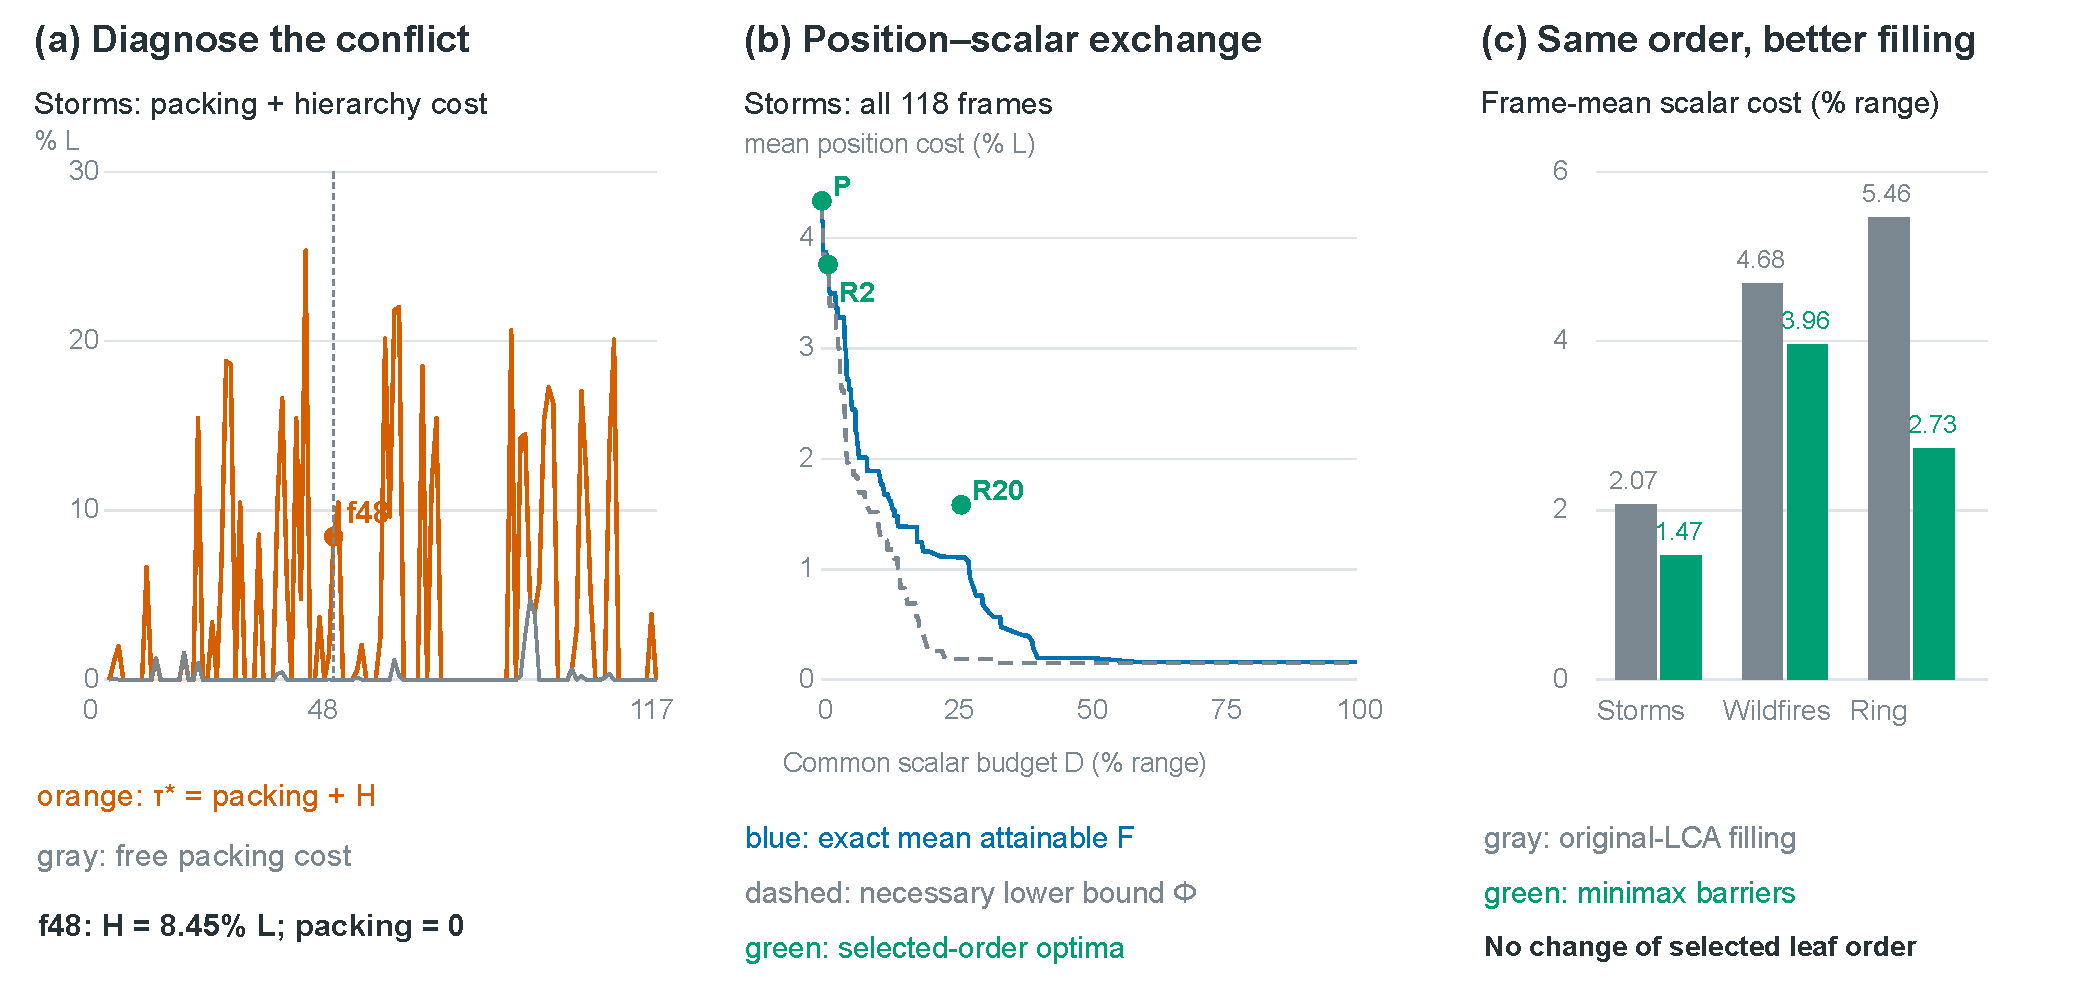
\includegraphics[width=\linewidth]{figures/Supplement_PositionScalarDiagnostic.pdf}
\caption{Additional certificate and filling diagnostics retained from the preceding revision. (a) Storms interval certificate, free packing cost, and the frame-48 hierarchy conflict. (b) Common-budget mean frontier and selected-order working points. (c) Mean original-LCA and optimal scalar costs for the same selected R20 orders. These supporting diagnostics accompany the five-panel main-paper frontier overview.}
\label{fig:s_certificate_fill}\end{figure}

\subsection{Storms three-snapshot detail}
The following retained four-method comparison complements Figure~1's separate hourly overview and eligibility-window comparison. It adds source snapshots at frames 47, 48, and 49 using identical colours and true extremum positions. Missing features are unmarked; $A=60$ begins at frame 48. Baseline axes remain native layout ranks, and dashed references occur only in RG panels.
\begingroup
\setlength{\intextsep}{6pt}
\begin{figure}[H]\centering
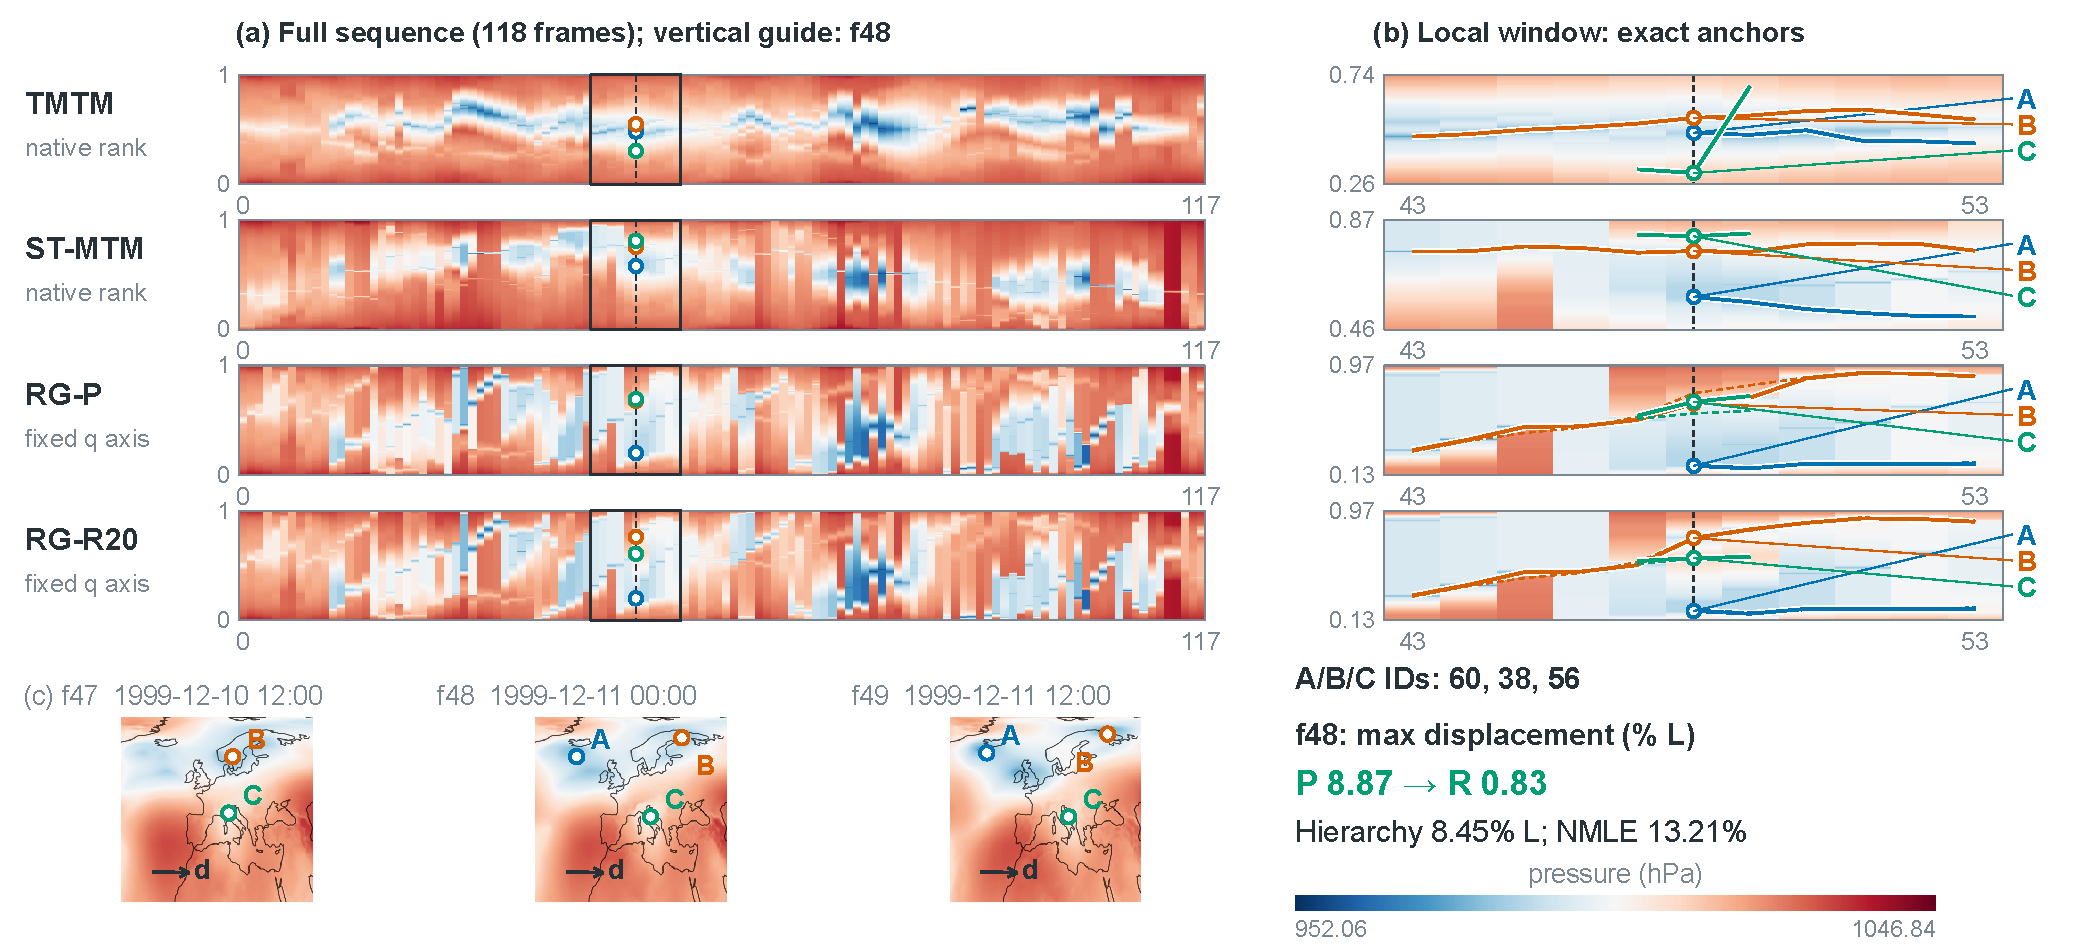
\includegraphics[width=.90\linewidth]{figures/Supplement_Storms_Detail.pdf}
\caption{Storms detail for the 118-frame quantitative sequence: four layouts, the local conflict window, and raw source snapshots with saved processed extrema. Tracks $A=60$, $B=38$, and $C=56$ refer to this sequence. Main-paper Figure~1 instead uses a separate 744-hour pressure-anomaly visualization with its own extracted features and track identifiers; the two populations and scalar preprocessing are distinct.}
\end{figure}
\endgroup

\paragraph{Storms eligibility and fixed-order scalar cost.} At frame 48, the $A/B$ node's parent gap is 15.314\,hPa and meets the eligibility threshold $\kappa=19.016$\,hPa. Its half-gap lower bound is 7.657\,hPa. Fixing $C$'s extremum value at 1006.693\,hPa raises the chosen order's analytical optimum to 12.557\,hPa; strict-extremum clearance produces the independently measured 12.558\,hPa error. These quantities respectively describe eligibility, a necessary bound, the fixed-order optimum, and the rendered result.


\subsection{Detailed measurements accompanying the Results section}
\paragraph{Storms frame 48.} Tracks $A=60,B=38,C=56$ have normalized references 0.208, 0.759, 0.603. TMTM orders them $C,A,B$, ST-MTM/P use $A,B,C$, and R20 uses $A,C,B$. All-leaf NROE is 19.734\%, 7.779\%, 7.779\%, and zero, respectively. Maximum P/R displacement is 8.867\%/0.833\% of $L$. Source merges are 994.136\,hPa for $A/B$ and 1009.449\,hPa for either outside pair; R places all three at 1006.694\,hPa.

\paragraph{Wildfires frames 17--19.} Track $C=52$ has fixed reference 0.418, P anchors 0.281, 0.549, 0.325, and R anchors 0.468, 0.422, 0.409. At frame 18, $A=3,B=48,C=52$ have references 0.169, 0.685, 0.418. Hierarchy cost is $13.921\%L$; maximum P/R displacement is $14.754\%/2.633\%L$. All-leaf NROE for TMTM/ST-MTM/P/R20 is 38.026\%/38.026\%/13.318\%/1.587\%. The $A/B$ source level 0.060800 changes to $-0.574262$, giving worst-pair error 0.635063 and 15.094\% actual NMLE.

\begin{samepage}
\paragraph{Tangaroa frame 140.} Tracks $A=432,B=462,C=388$ have references 0.291, 0.804, 0.534 and source joins 0.713403 ($A/B$), 0.869923 (either outside pair). TMTM/P/R20 order them $C,A,B$/$A,B,C$/$A,C,B$, with all-leaf NROE 15.529\%/13.495\%/0.532\%. Packing is $0.183\%L$, the hierarchy lower bound $13.744\%L$, and maximum P/R displacement $14.760\%/1.016\%L$. R sets $A/B$ to 0.988407 and $A/C$ to 0.594919: worst-pair change 0.275004, or 13.750\% actual NMLE.
\end{samepage}

\subsection{Annual PM2.5 source-linked case}
The current main-paper PM2.5 case is additional visual analysis of the existing 366-frame experiment; no date, grid, smoothing parameter, layout, match, or primary metric is replaced. Of 34 frames with a strongest three-feature witness exceeding $0.02L$, frames 185, 186, 195, 196, and 317 have the witness tracks present for at least three consecutive saved dates. Their median witness obstruction selects frame 195 (July 14), with bound $10.2575\%L$. The three tracks coexist on frames 195--197. The displayed window is frames 191--201 (July 10--20), including all saved births and deaths. Supplied views are frames 193--197; no temporal averaging or additional smoothing is introduced for those images. Each file represents its recorded 10:30 field, without an established daily averaging interval.

The July 14 measurements use displayed raster anchors, rather than the continuous-coordinate $E_\infty$ of the main sequence table. Exact source-array checks give maximum P/R20 errors $14.8809\%L$/$0.8373\%L$. Source/P pair levels are 25.936435 ($A/B$) and 22.626129 ($A/C,B/C$); R20 uses 24.281282 for all three. Direct labelled merge measurement yields 1.655153\,$\mu$g\,m$^{-3}$, normalized by the fixed annual processed range 147.885866\,$\mu$g\,m$^{-3}$, or 1.119210\% NMLE. The window maximum is 3.332004\%. Colour scales are shared within panels: 0--165 for the annual map and 0--100\,$\mu$g\,m$^{-3}$ for all local supplied/processed views and P/R20 maps. These display ranges do not redefine NMLE normalization. Province outlines are geographic context only.

The case selection, complete candidates, source hashes, marker coordinates, saved lifetimes, scalar comparisons, and display-reconstruction checks are packaged in \path{evidence/pm25_case20261023/}. The annual P/R20 primary motion errors remain 42/95 and 47/95. A local reference-alignment example is not a physical-event validation or an annual performance estimate.

\section{Additional Reference-Dataset Experiments}\label{sec:additional_experiments}
This section documents the Nucleon, Cylinder, and reconstructed Benzene additions independently of the 614-frame planar suite, the 744-hour Storms visualization, the 64-frame mirror control, and the 201-frame Tangaroa experiment. Existing measurements and figures are retained. Saved result records and their SHA-256 bindings are packaged under \path{evidence/additional_datasets/}. Every new dataset has \texttt{status=complete\_verified}; complete-map verification covers 5 Nucleon maps, 510 Cylinder maps, and 105 Benzene maps.

\subsection{Data correspondence and coverage}
\begin{table}[H]\centering\small
\caption{Correspondence with the six dataset families in TMTM. Coverage of a family does not imply identical final author inputs.}\label{tab:s_reference_coverage}
\begin{tabular}{lll}\toprule
Name & Current input & Correspondence / scope\\\midrule
Nucleon & $64\times64$, 1 slice & Original author padded slice; static\\
Ring & $14\times14$, 40 frames & Archived author generator\\
Storms & $49\times49$, 744 hours & ERA5 anomaly overview; 118-frame statistics separate\\
Tangaroa & $300\times180\times120$, 201 volumes & Author source; declared speed and TTK protocol\\
Cylinder & $135\times64\times48$, 102 volumes & Public resampling; reference reports 508 frames\\
Benzene & $61\times61$, 21 $z$ sections & Reconstructed OPLS-AA electrostatic potential\\
\bottomrule\end{tabular}\end{table}
The Benzene author potential file remains unavailable; the newly accepted reconstruction supplies a related scalar model rather than its original fractional-charge calculation. The earlier electron-density and two-dimensional circular-cylinder pilots are excluded. Cylinder remains a genuinely three-dimensional spatial input, while Benzene is a sequence of two-dimensional spatial sections of a static field.

\subsection{Shared construction and numerical scope}
All five methods in each new experiment share the same processed fields, extracted extrema, supports, and overlap correspondences. The historical configurations compare TMTM, RG-MTM-P, and RG-MTM-R at eligibility fractions 0.02, 0.20, and 1.00. A subsequent run adds ST-MTM on every retained input; its complete primary and SNS/TW/TD metrics are reported in the current main tables and S3. Historical tables below retain their original configuration scope. The reference is fixed to the physical $x$ axis. Scalar normalization uses one sequence-wide range, with no per-frame scalar normalization. NROE uses the full leaf population and NMLE is independently measured on complete saved profiles. A figure preview is not a metric input.

Nucleon and Cylinder use a join tree of the negated, scaled source scalar, equivalent to its split tree; displayed values recover the original sign and units. Benzene instead uses the positive, scaled potential and its join tree. A sign inversion is not silently reused across these datasets. The RG raster has 32768 rows; TMTM retains every input sample with its declared virtual saddle multiplicities. At most four declared legal orders enter the secondary convex optimization. Relaxation pruning is disabled; bounds and finite candidate sets do not imply global secondary optimality.

Independent verification checks scalar transforms, augmented-tree sample ownership and monotone arcs, parent-chain LCAs, full-map barriers, TMTM sample multiplicities, and RG hard constraints. Cylinder additionally recomputes all three-dimensional $Q$ values using an independent Amira parser and the rotation/strain Frobenius-norm identity. Benzene recomputes all 78,141 source-potential samples using scalar distances and \texttt{math.fsum}; saved float32 source values agree exactly. Native TTK still supplies persistence simplification, which is not independently reimplemented by these audits. No new claim about cross-hardware runtime or perceptual accuracy is made.

\subsection{Nucleon protocol}
The source is the TMTM author's padded uint8 centre slice from the archived author revision recorded in the packaged input protocol. It is used without smoothing, spatial resampling, or persistence removal. Scalar range is 247, and $x,y=0,\ldots,63$. The extracted input has 13 leaves and 26 nodes versus 28 nodes in the reference table. This mismatch is retained rather than tuning the input to match the published count. All three R maps are exactly equal to the saved P array. One static slice cannot support temporal or volumetric claims.

\subsection{Benzene reconstructed potential}
The declared 12-site vacuum Coulomb model is $V(r)=\sum_iq_i/\|r-R_i\|$, with six carbon charges $-0.115e$ and six hydrogen charges $+0.115e$ from Table 1, page 67 of the BOSS 4.9 manual~\cite{Jorgensen:2013:BOSS}. The public Inviwo molecular cube supplies atomic coordinates only~\cite{Inviwo:BenzeneGeometry}; no electron-density samples are interpreted as potential. Coordinates are in bohr and potential is in Hartree/$e$. No softening radius, clipping, smoothing, charge fitting, or post hoc symmetry enforcement is applied. The minimum grid-to-charge distance is 0.0519513 bohr, so the sampled grid avoids singularities. The model, geometry, and domain were fixed before layout comparison.

Each $61\times61$ section spans $[-6,6]^2$, and 21 parallel sections span $z=-2,-1.8,\ldots,2$. The signed potential is divided by one fixed range 3.92116975784 before join-tree extraction. Traditional persistence simplification uses 0.05\% of each section's range. There are 5--10 leaves and 10--20 nodes, versus the reference table's 14--68 nodes. Four leaf extrema lie on the rectangular boundary in every section. An interior-extremum diagnostic uses only the 15 sections with at least two interior leaves; this is distinct from whether a leaf's support touches the boundary. Full-population results remain primary.

The source geometry is nearly planar rather than exactly planar: the maximum $\pm z$ source-field discrepancy is 0.0241\% of the sequence range. The map mirror diagnostic compares ten $\pm z$ pairs at the same 32768 common map coordinates, without a fitted reflection or alignment. Adjacent-section displacement residual is the absolute difference between displayed anchor change and projected-source change divided by domain width; all methods share 170 overlap matches. These quantities measure section coherence and approximate reflection, not physical molecular motion. The Benzene comparison in S10 uses a common coolwarm symmetric-log display, linear inside $\pm0.0784234$ a.u., with fixed endpoints $\pm2.20763588$ a.u. The display does not change scalar arrays. TMTM is not optimized for the prescribed $x$ reference; its NROE is a reference-compatibility diagnostic rather than its original objective.

\subsection{Cylinder input, motion, and rendering}
The velocity archive is the public uniformly resampled square-cylinder simulation credited to Camarri, Salvetti, Buffoni, and Iollo~\cite{Camarri:2005:Cylinder,Weinkauf:SquareCylinder,Funck:2008:Smoke}. Spatial derivatives use physical coordinates on the full $192\times64\times48$ source grid. Only afterward are source $x$ indices 57--191 retained, giving $x\in[-2.45026178,20]$, $y\in[-4,4]$, and $z\in[0,6]$. All 102 archive members are used. There is no smoothing, downsampling, or leaf-count filtering. The source is spanwise-periodic, but this implementation does not connect the $z$ endpoints: it uses second-order one-sided derivatives at boundaries and marks boundary-touching features. This treatment and the 102-versus-508-frame difference limit equivalence to the original paper's final $Q$ fields.

Persistence simplification uses 2\% of each source frame's range. The fixed sequence scalar scale is 25.8113212585. The retained trees have 8--150 nodes and 4--75 leaves. Motion uses overlap-linked extrema, a two-step window, and a 2\%-of-domain-diagonal change threshold for three-dimensional truth. The projected diagnostic uses 2\% of the $x$ extent and has its own clear-event population. Error counts and exact projection are given below. Neither diagnostic is a physical vortex-label ground truth.

The maps use the saved 2048-row previews with no additional point or trajectory overlay. Coolwarm is normalized by a shared symmetric logarithm, linear inside $[-0.02,0.02]$, with fixed endpoints $\pm20.4634399414$. Main Figure~16 shows raw source isosurfaces at $Q=0.1$ and $0.5$ for the fixed first, middle, and last snapshots (frames 0, 51, 101). Marching cubes uses the original physical grid and no smoothing. The camera is orthographic, elevation $22^\circ$, azimuth $-65^\circ$; physical aspect, levels, and opacity are fixed across all views. Native domain edges project the same eight physical corners. These source views precede TTK simplification, while the maps show the common processed scalar and method-specific filling. Rendering records and source-frame hashes are in \path{evidence/additional_datasets/render_metadata.json}.

\subsection{Complete two-dimensional measurements}
\begin{table}[H]\centering\small
\caption{Nucleon static input: complete saved configuration comparison. NROE and NMLE are percentages.}
\begin{tabular}{lrrrr}\toprule Method & NROE & NMLE mean & NMLE max & Exact-topology frames\\\midrule
TMTM & 11.9048 & 0.0000 & 0.0000 & 1/1\\
RG-MTM-P & 2.3810 & 0.0000 & 0.0000 & 1/1\\
RG-MTM-R2 & 2.3810 & 0.0000 & 0.0000 & 1/1\\
RG-MTM-R20 & 2.3810 & 0.0000 & 0.0000 & 1/1\\
RG-MTM-R100 & 2.3810 & 0.0000 & 0.0000 & 1/1\\
\bottomrule\end{tabular}\end{table}

\begin{table}[H]\centering\small
\caption{Benzene 21 reconstructed-potential sections: complete saved configuration comparison. NROE and NMLE are percentages.}
\begin{tabular}{lrrrr}\toprule Method & NROE & NMLE mean & NMLE max & Exact-topology frames\\\midrule
TMTM & 50.0000 & 0.0000 & 0.0000 & 21/21\\
RG-MTM-P & 4.2063 & 0.0000 & 0.0000 & 21/21\\
RG-MTM-R2 & 0.0000 & 0.0025 & 0.0080 & 6/21\\
RG-MTM-R20 & 0.0000 & 0.0025 & 0.0080 & 6/21\\
RG-MTM-R100 & 0.0000 & 0.0025 & 0.0080 & 6/21\\
\bottomrule\end{tabular}\end{table}

\begin{table}[H]\centering\small
\caption{Benzene boundary and section-coherence diagnostics, all in percent. Interior NROE uses 15 eligible sections; residual uses 170 adjacent-section matches; mirror MAE uses ten section pairs. The full-population table above remains primary.}
\begin{tabular}{lrrr}\toprule Method & Interior NROE & Displacement residual & Mirror-map MAE\\\midrule
TMTM & 12.5000 & 2.7546 & 0.0185\\
RG-MTM-P & 5.8889 & 1.2191 & 0.0064\\
RG-MTM-R2 & 0.0000 & 0.1373 & 0.0030\\
RG-MTM-R20 & 0.0000 & 0.1373 & 0.0030\\
RG-MTM-R100 & 0.0000 & 0.1373 & 0.0030\\
\bottomrule\end{tabular}\end{table}

\subsection{Complete three-dimensional measurements}
\begin{table}[H]\centering\small
\caption{Cylinder 102 three-dimensional fields: complete saved configuration comparison. NROE and NMLE are percentages.}
\begin{tabular}{lrrrr}\toprule Method & NROE & NMLE mean & NMLE max & Exact-topology frames\\\midrule
TMTM & 26.6169 & 0.0000 & 0.0000 & 102/102\\
RG-MTM-P & 12.2622 & 0.0000 & 0.0000 & 102/102\\
RG-MTM-R2 & 0.2488 & 0.6919 & 4.8865 & 8/102\\
RG-MTM-R20 & 0.0841 & 2.8096 & 14.2811 & 5/102\\
RG-MTM-R100 & 0.0841 & 3.1901 & 14.2811 & 5/102\\
\bottomrule\end{tabular}\end{table}

\begin{table}[H]\centering\small
\caption{Cylinder motion proxies. Three-dimensional truth has 3196 clear events; projected truth has 2934. Counts show reversal + miss. Exact projection has no rendered scalar topology and is a reference control.}
\begin{tabular}{lrrrr}\toprule Method & 3D count & 3D error (\%) & Projected count & Projected error (\%)\\\midrule
TMTM & 845+1296 & 66.990 & 867+978 & 62.883\\
RG-MTM-P & 598+593 & 37.265 & 510+360 & 29.652\\
RG-MTM-R2 & 76+541 & 19.305 & 0+123 & 4.192\\
RG-MTM-R20 & 71+534 & 18.930 & 0+108 & 3.681\\
RG-MTM-R100 & 72+534 & 18.961 & 0+107 & 3.647\\
Exact $x$ projection & 69+534 & 18.867 & 0+0 & 0.000\\
\bottomrule\end{tabular}\end{table}

\paragraph{Optimization records.}
\begin{center}\small
\begin{tabular}{lrrr}\toprule
Dataset & Max. bracket / $L$ & QP gap / $L^2$ & Failed QPs\\\midrule
Nucleon & $1.926\times10^{-10}$ & $8.382\times10^{-8}$ & 0\\
Cylinder & $0.00830968$ & $7.037\times10^{-6}$ & 0\\
Benzene & $1.985\times10^{-10}$ & $8.957\times10^{-7}$ & 0\\
\bottomrule\end{tabular}\end{center}
A finite certificate gap remains on some Cylinder cases. Verification establishes the stated saved-map and feasibility checks rather than exact continuous optimality of every certificate or a global optimum over all secondary orders.

\clearpage
% Keep the section opening with its first comparison.
\section{Complete Visual Comparisons and Hierarchical Ordering}\label{sec:full_visual_comparisons}
The main paper focuses on RG-MTM-P/R and their source fields. This section retains the complete shared-input comparisons with TMTM and ST-MTM, additional source sections, and the clustering-hierarchy example. All panels use the same frozen scientific arrays as the main results. The baselines are local reimplementations, rather than images copied from the reference publications.

\subsection{Two-dimensional inputs and controls}
\begin{figure}[H]
\centering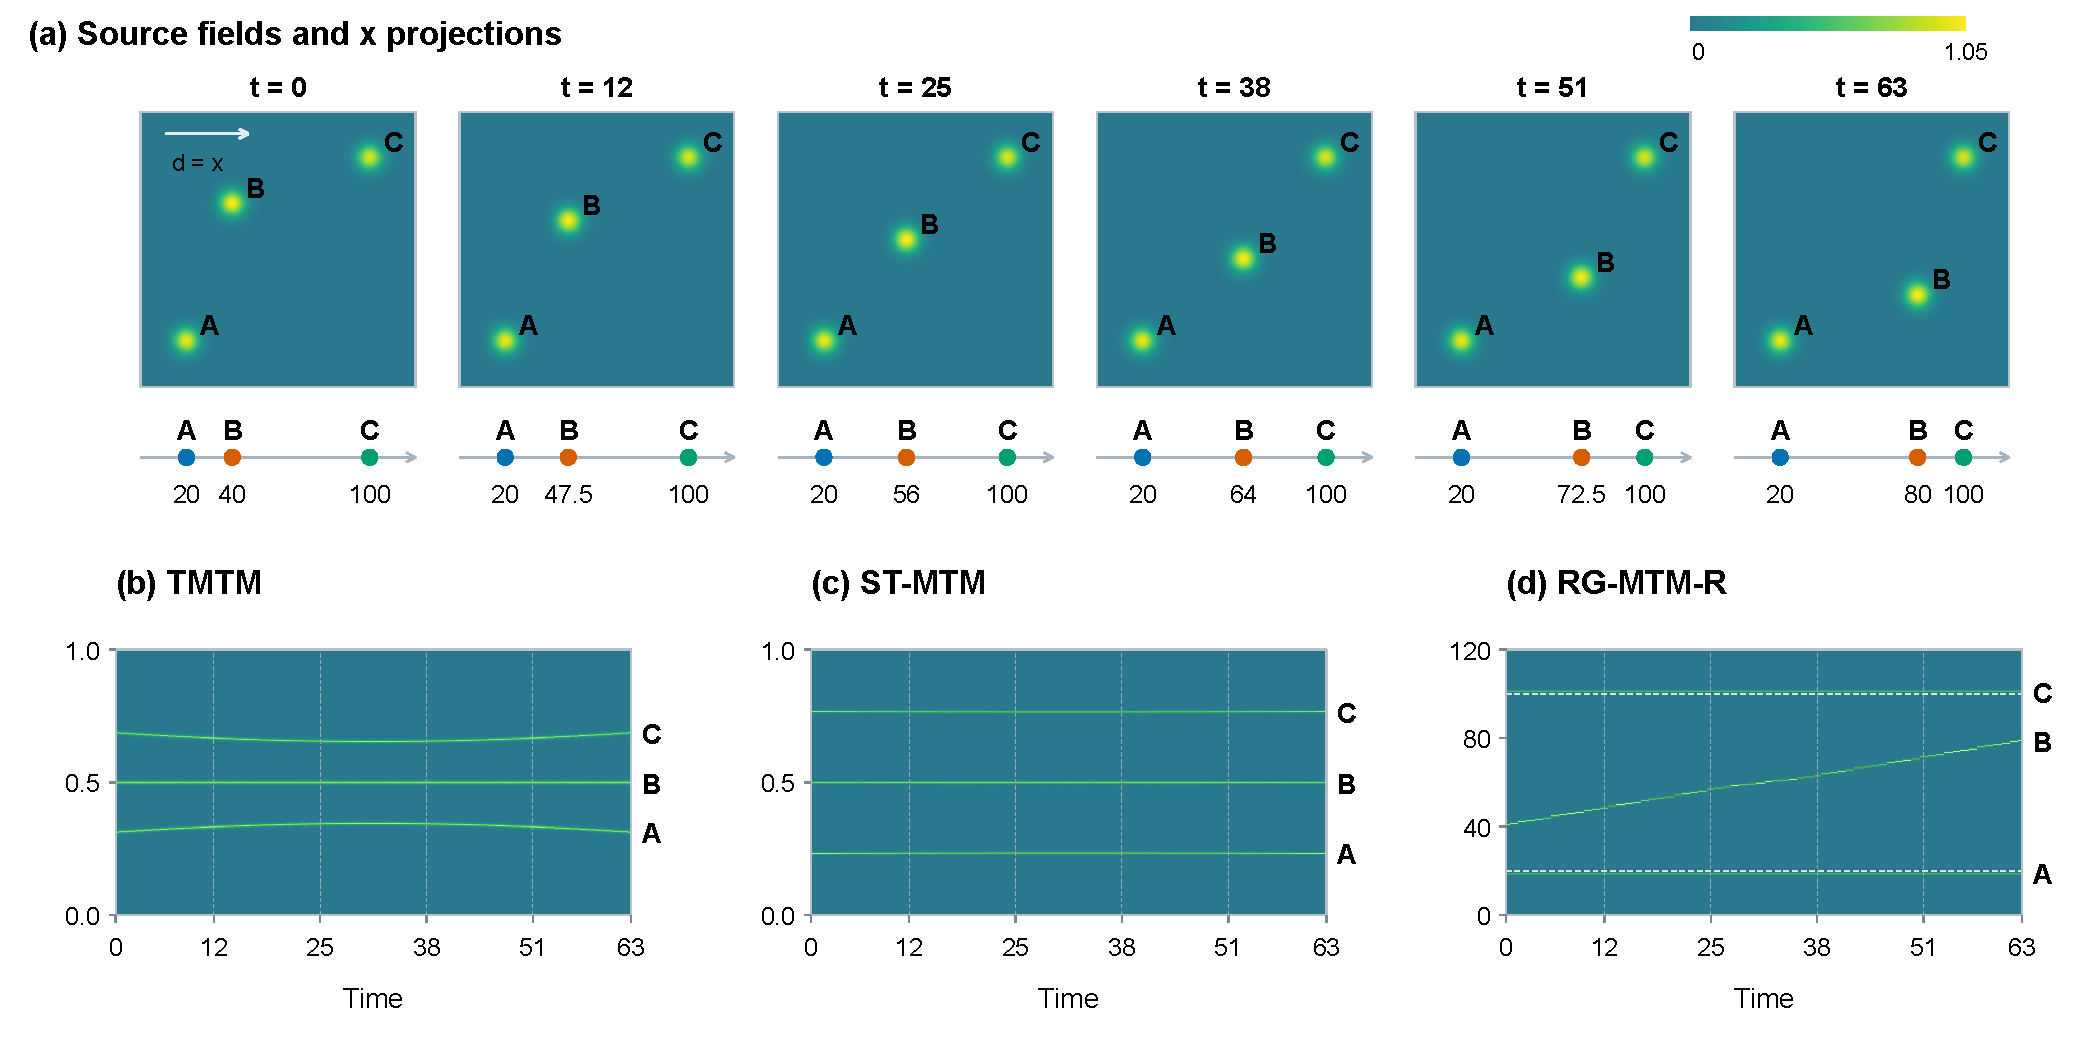
\includegraphics[width=\linewidth]{figures/Supplement_ReferenceControl_Full.pdf}
\caption{Relative distances and absolute reference position. (a) Six source fields and $x$ projections follow moving $B$ between fixed $A,C$; mirror endpoints preserve pairwise distances while changing horizontal position. (b,c) TMTM/ST-MTM use internal map coordinates. (d) RG-MTM-R uses source $x$ units, with dashed fixed references. Source peaks and temporal bands share a linear 0--1.05 scalar scale. Vertical guides mark source-frame times. All three preserve merge levels; position errors and calibration are reported in the main paper's absolute-reference control.}
\label{fig:s_full_bisector_three_methods}
\end{figure}

\begin{figure}[H]
\centering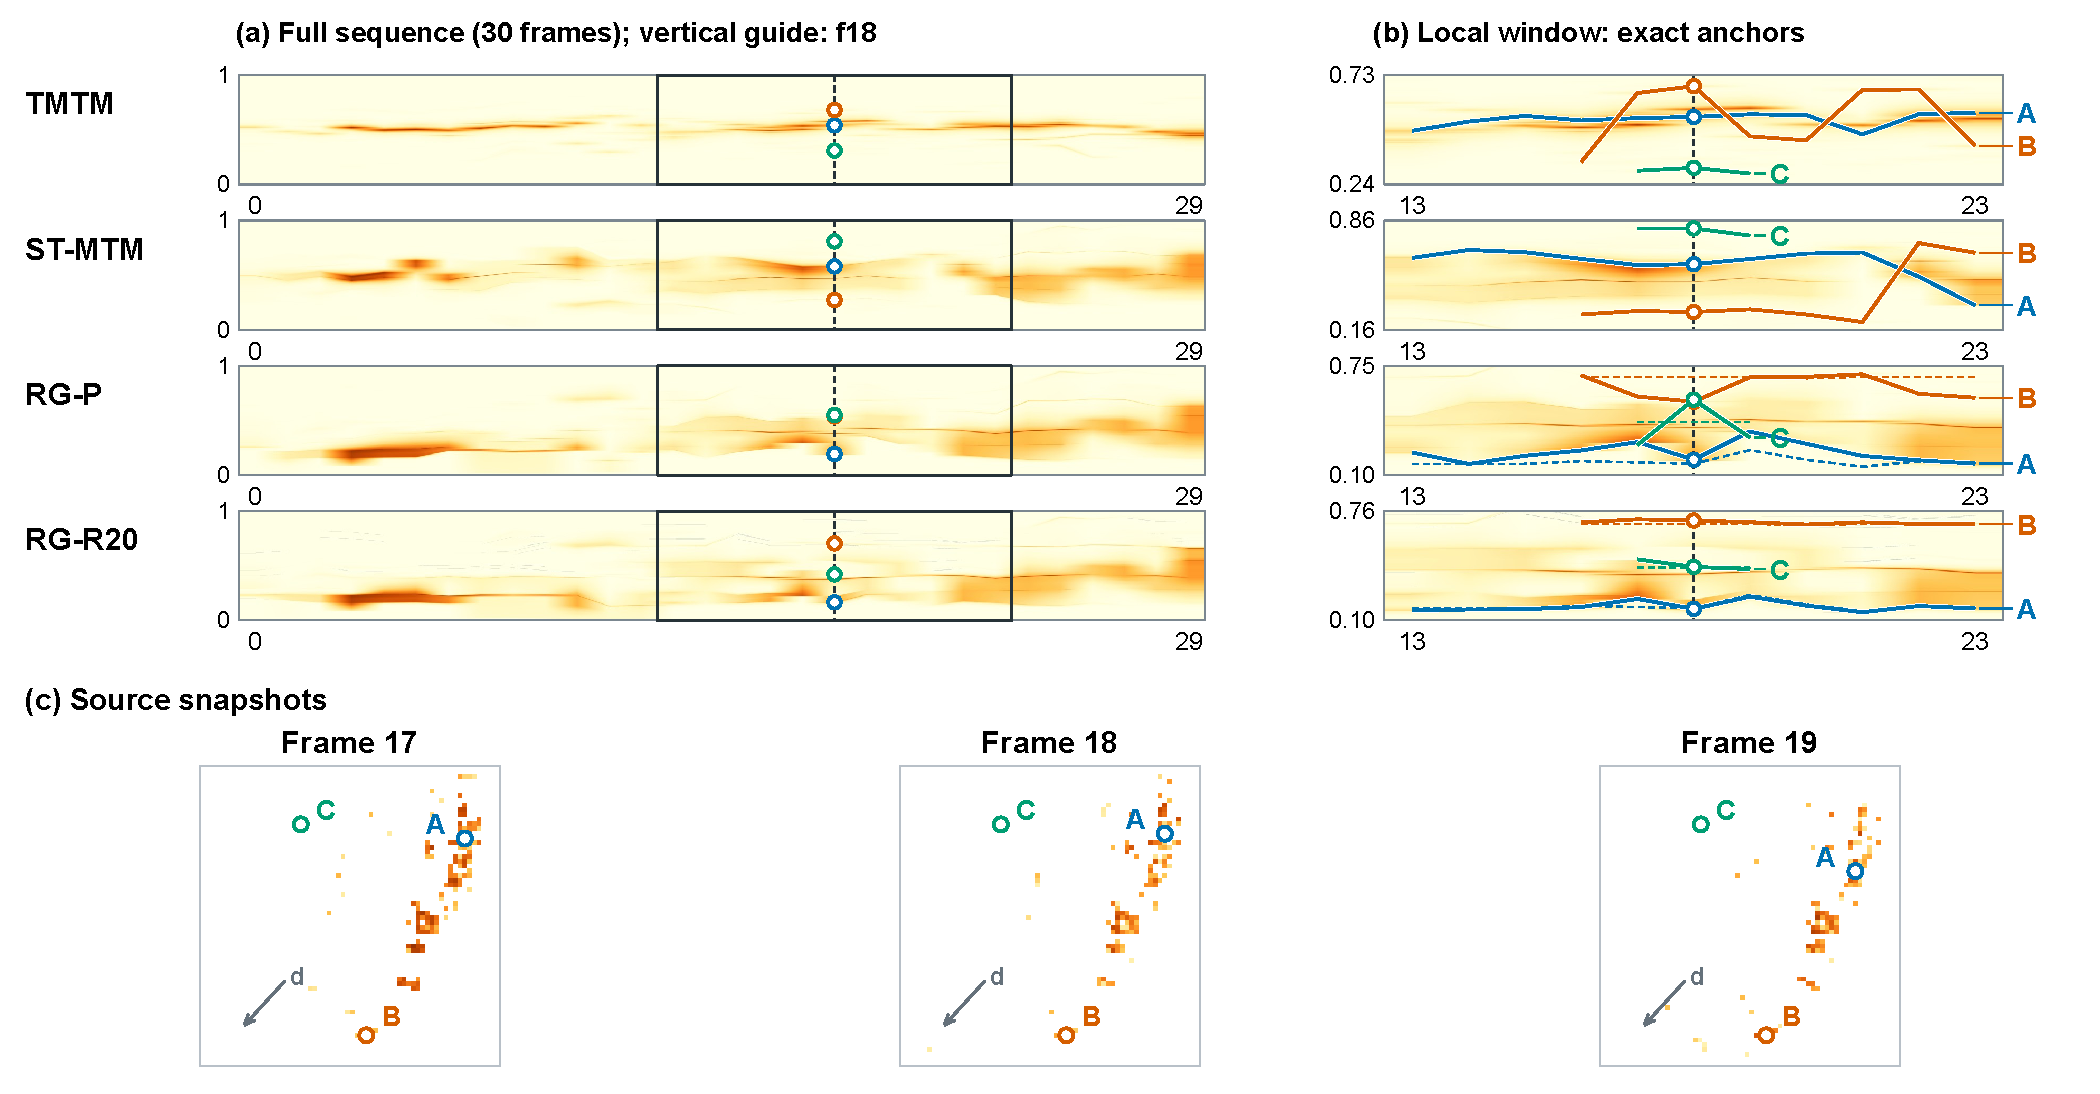
\includegraphics[width=\linewidth]{figures/Supplement_Wildfires_Comparison.pdf}
\caption{Wildfires source events and four layouts. Complete 30-frame maps (left) and frames 13--23 (right) share tracks $A=3$, $B=48$, $C=52$. Circles and solid traces show saved anchors; dashed RG traces show references. Baseline axes are native rank; RG axes use the fixed projection. Local ordinate ranges are labelled. Bottom: two-date FRP sums aggregated onto the $64\times64$ grid and transformed by $\log(1+\mathrm{FRP}/\mathrm{MW})$, before smoothing, at frames 17--19. These are binned records rather than untouched satellite observations or burn perimeters. The overlaid markers locate processed extrema. The main wildfire figure separately displays the supplied 10-km cell polygons with geographic context and the corresponding smoothed analysis fields. At frame 18, P/R maximum displacement is 14.75\%/2.63\% of reference extent, at 15.09\% actual R NMLE. A yellow--orange--brown scale encodes log-FRP with fixed ranges 0--4.21 for processed maps and 0--12.05 for binned snapshots. Grey-blue denotes artificial negative connections. Temporal colour maps use display interpolation only; source snapshots and all original evaluation samples are unchanged.}
\label{fig:s_full_wildfires_events}
\end{figure}

\begin{figure}[H]
\centering\includegraphics[width=\linewidth]{figures/Supplement_OLR_Comparison.pdf}
\caption{OLR: complete 60-frame frozen method maps on one scalar scale. Baseline ordinates are native sample rank, while P/R use the fixed reference; normalization of the displayed axes does not make their meanings identical. The common primary motion record gives P and R20 the same total of 3/56 errors, despite improved reference order. No local temporal crop is selected.}
\label{fig:s_olr_complete}\end{figure}
\begin{figure}[H]
\centering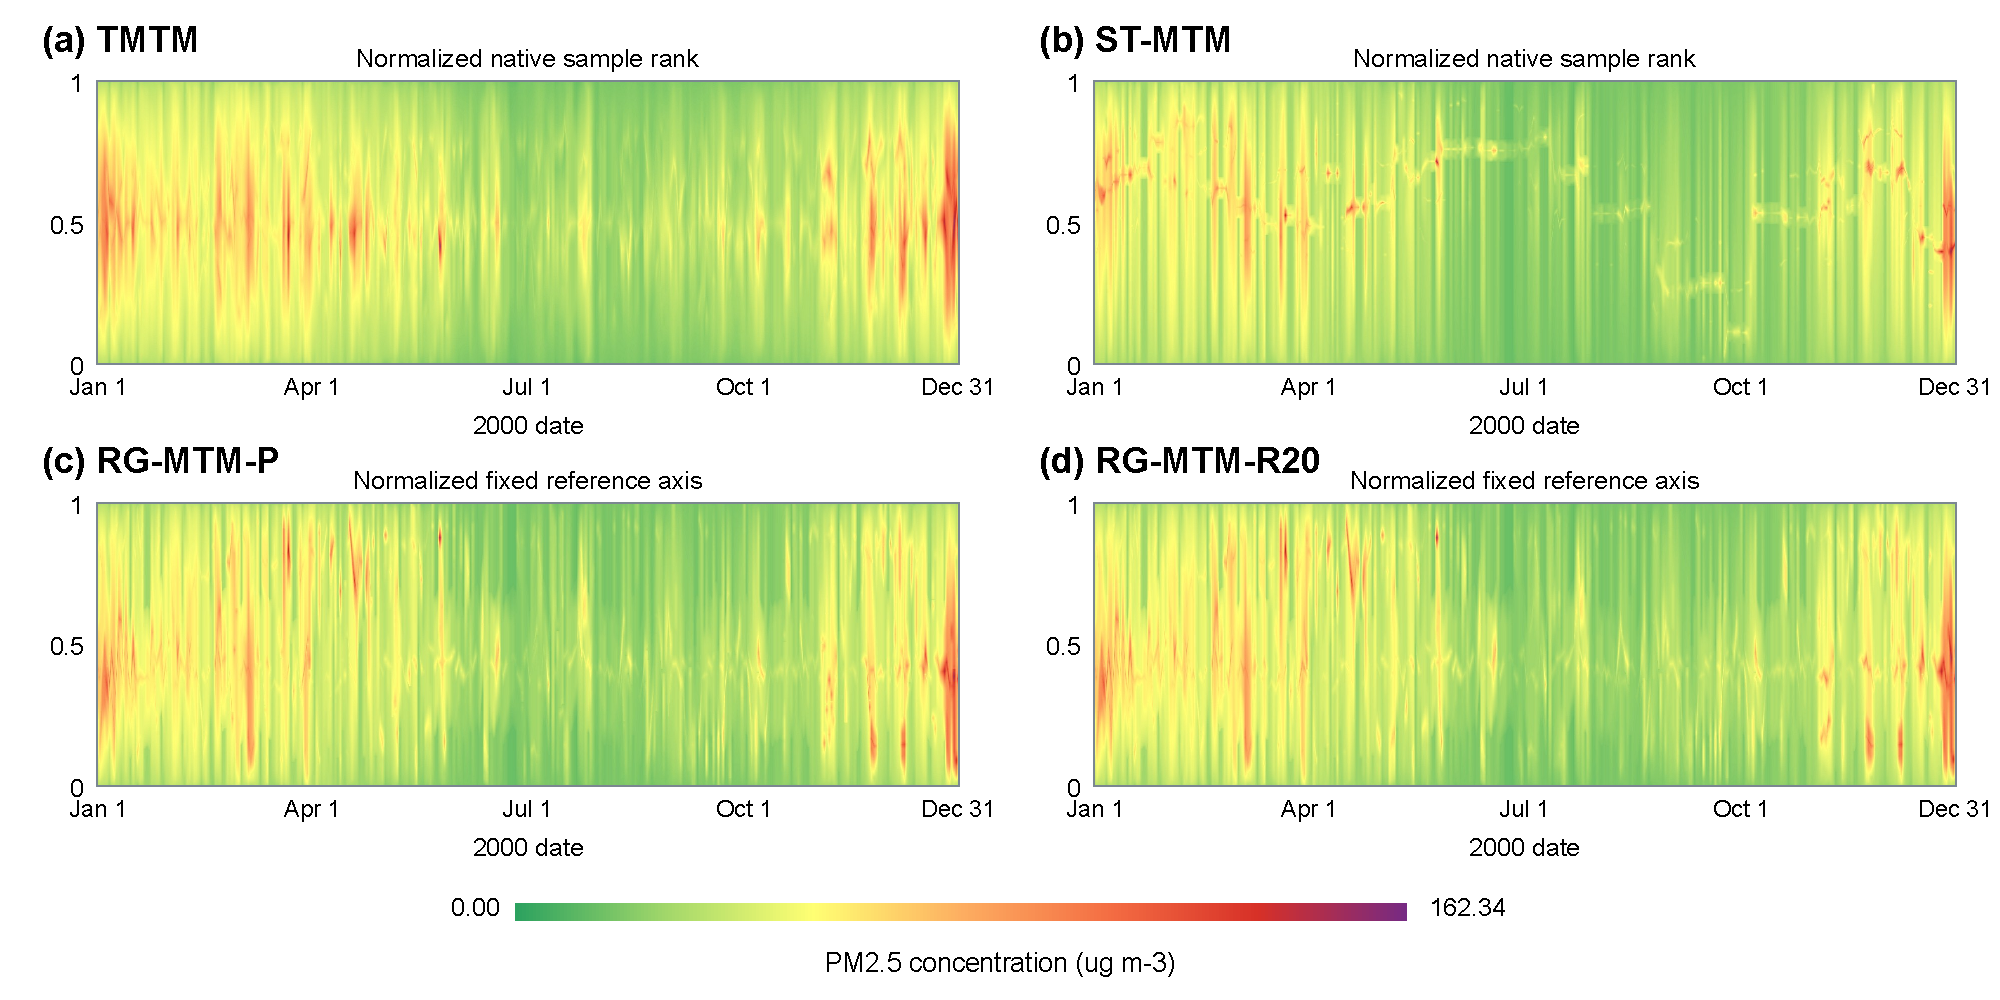
\includegraphics[width=\linewidth]{figures/Supplement_PM25_Comparison.pdf}
\caption{PM2.5: complete 2000 sequence (366 fields) for TMTM, ST-MTM, P and R20. All methods share the same processed inputs. Native baseline rank axes differ from the fixed RG reference axis. The shared pollution palette encodes concentration, not AQI. Conservative interpolation preserves every saved profile; metrics use original arrays. P/R20 motion errors are 42/95 and 47/95 on continuous anchors. The annual result replaces the earlier January display.}
\label{fig:s_pm25_complete}\end{figure}

\begin{figure}[H]
\centering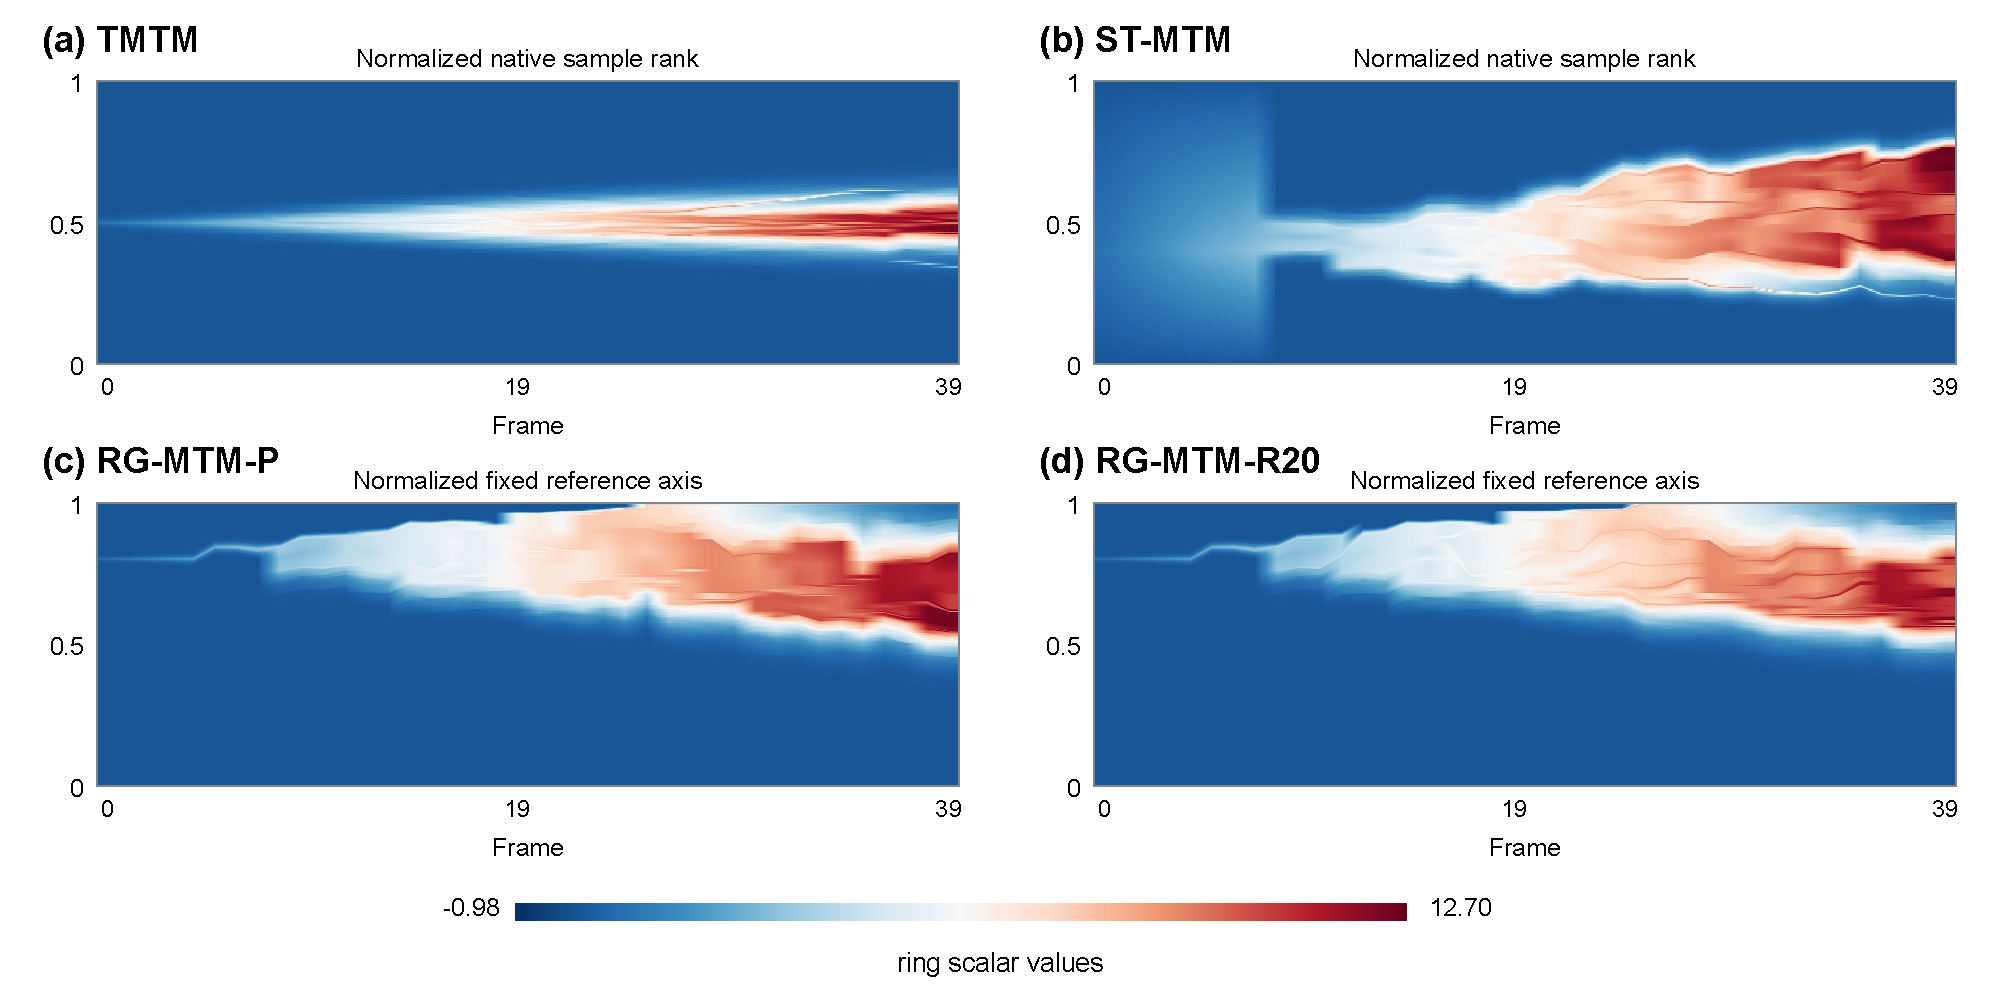
\includegraphics[width=\linewidth]{figures/Supplement_Ring_Comparison.pdf}
\caption{Ring: all 40 saved frames for TMTM, ST-MTM, P, and R20 on a shared scalar scale. Baseline ordinates are normalized native sample rank; P/R use the fixed spatial reference. Their meanings remain distinct. R20 improves the primary spatial-motion proxy from P's 39/124 to 16/124 at 2.73\% mean NMLE. This is the archived author ring generator on a $14\times14$ grid. Source hashes and zero cross-method scalar residuals at 165 saved feature anchors bind the displayed cache to the retained experiment; no layouts were recomputed.}
\label{fig:s_ring_complete}
\end{figure}

\begin{figure}[H]
\centering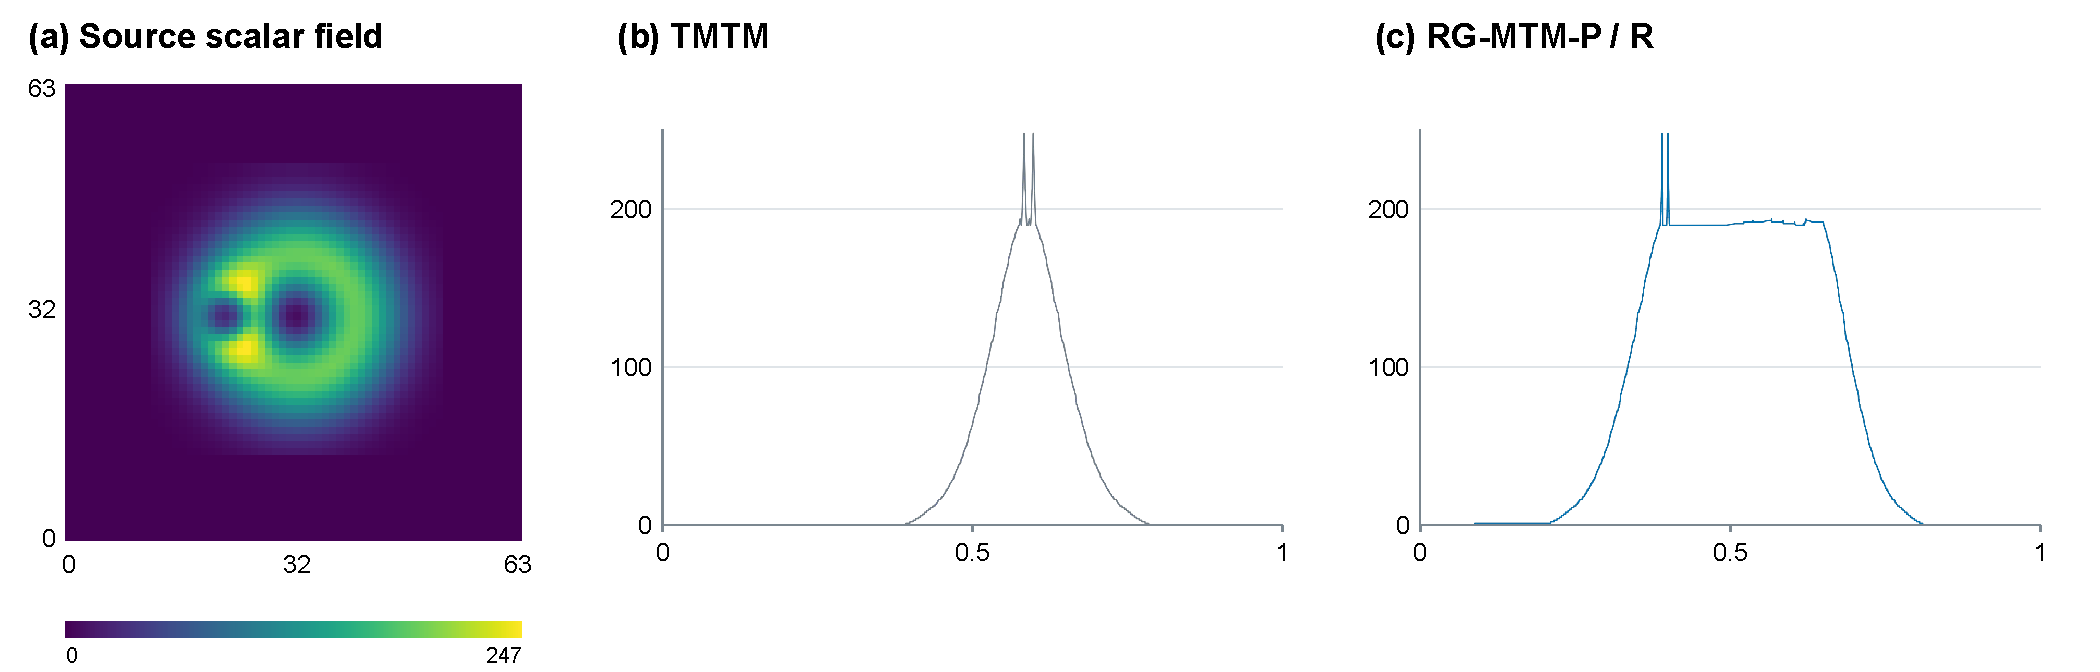
\includegraphics[width=\linewidth]{figures/Supplement_Nucleon_Comparison.pdf}
\caption{Nucleon static comparison. (a) The unchanged author $64\times64$ scalar slice. (b) Complete TMTM profile (4096 samples). (c) Complete P profile (32768 samples); all three R profiles are exactly identical to P. The source and curves use the original scalar units. NROE decreases from 11.90\% to 2.38\%, with zero measured NMLE throughout. This single frame supplies no temporal-motion or three-dimensional result.}
\label{fig:s_full_nucleon}
\end{figure}

\begin{figure}[H]
\centering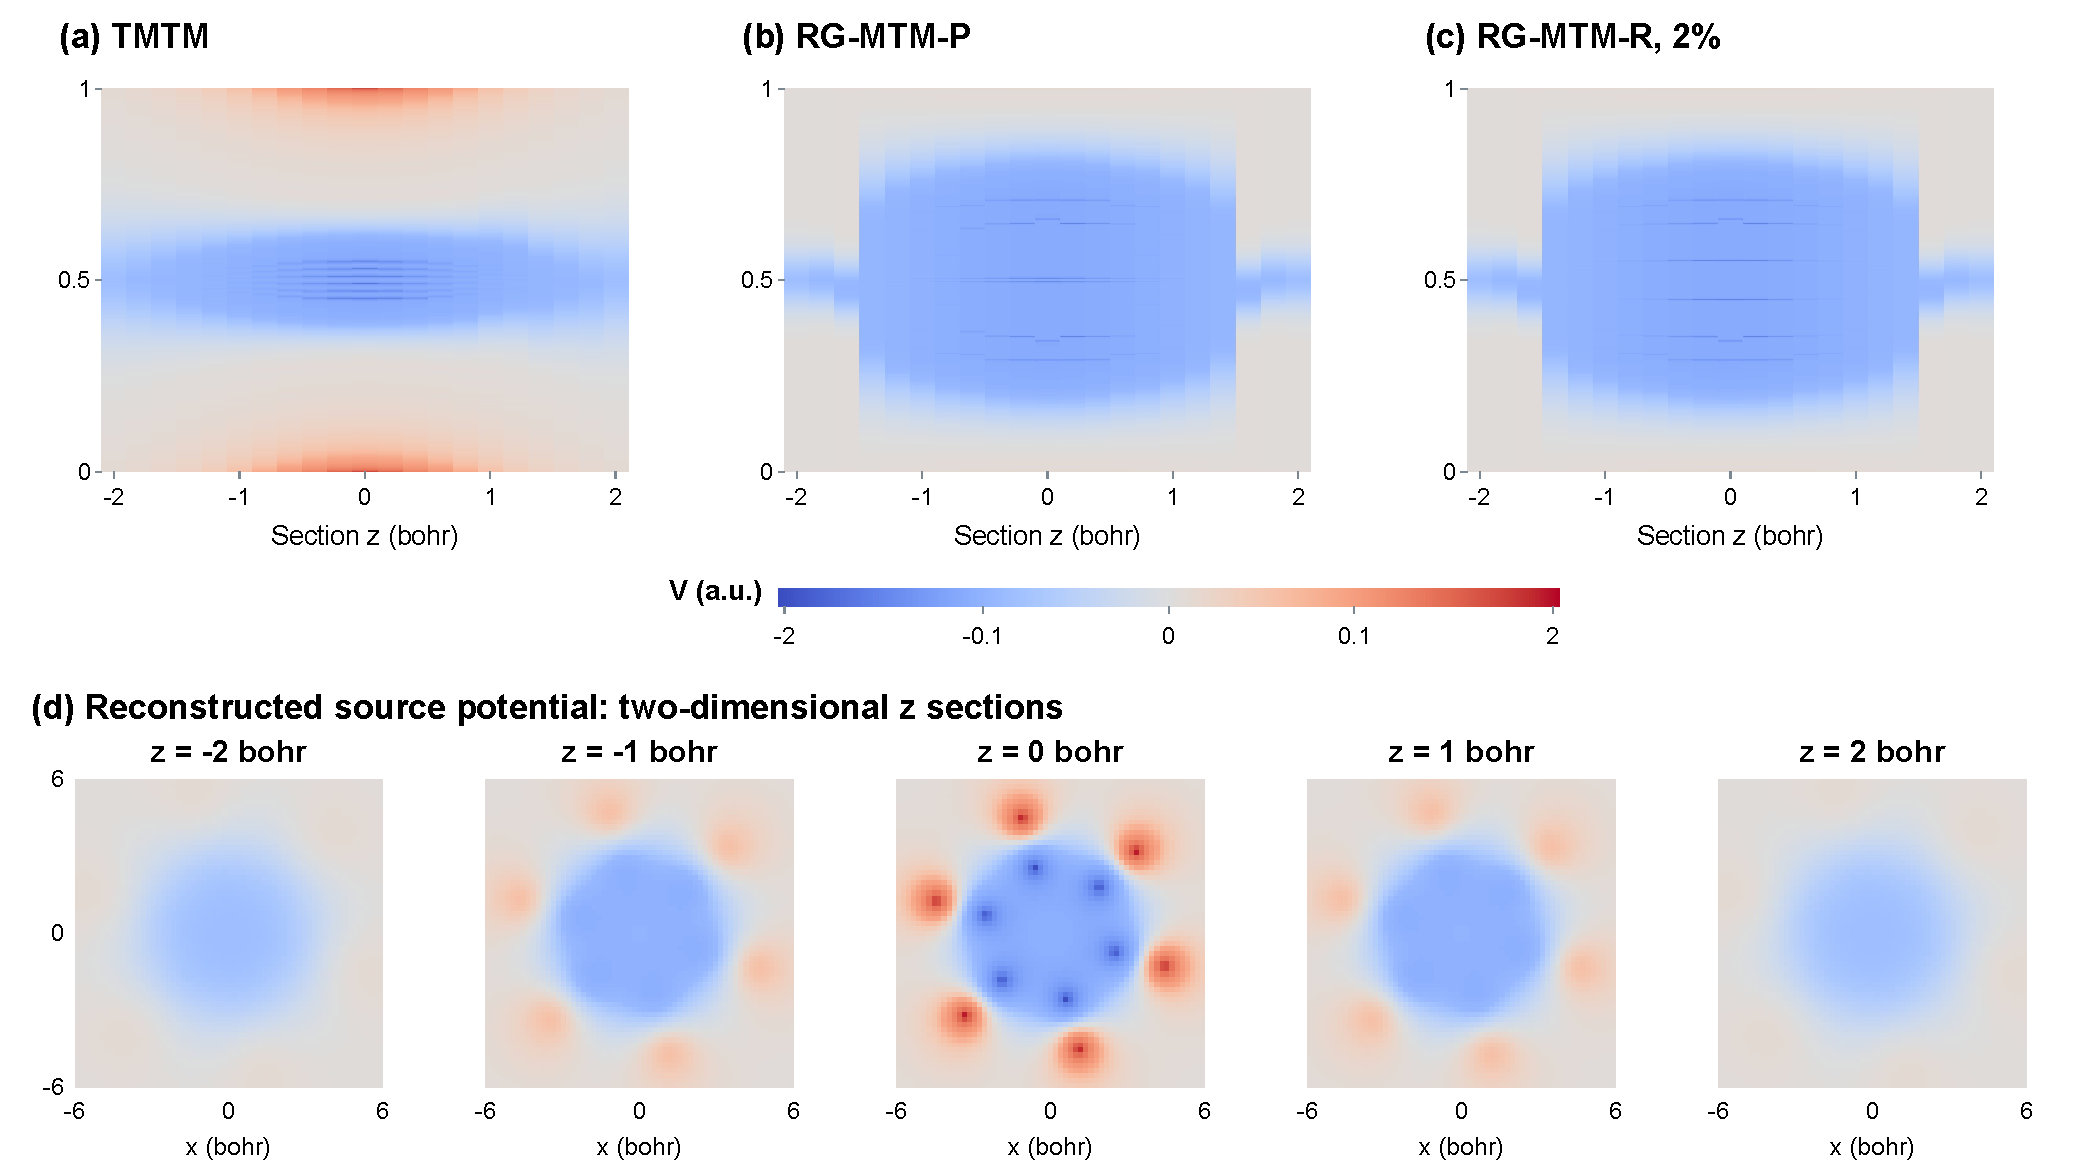
\includegraphics[width=\linewidth]{figures/Supplement_Benzene_Comparison.pdf}
\caption{Benzene reconstructed electrostatic potential. (a)--(c) Maps of all 21 static $z$ sections for TMTM, P, and R2; $z$ is not physical time. TMTM uses its native map coordinate, while RG uses normalized $x$ reference position. (d) Five $61\times61$ source-potential sections on the same symmetric-log colour scale (linear within $\pm0.0784$ a.u.). Values are in Hartree/$e$; source coordinates are in bohr. The field is the declared OPLS-AA point-charge reconstruction, not the original author's potential or electron density. Full-population scores retain four boundary extrema per section; internal-extremum diagnostics are reported separately.}
\label{fig:s_full_benzene}
\end{figure}

\begin{figure}[H]
\centering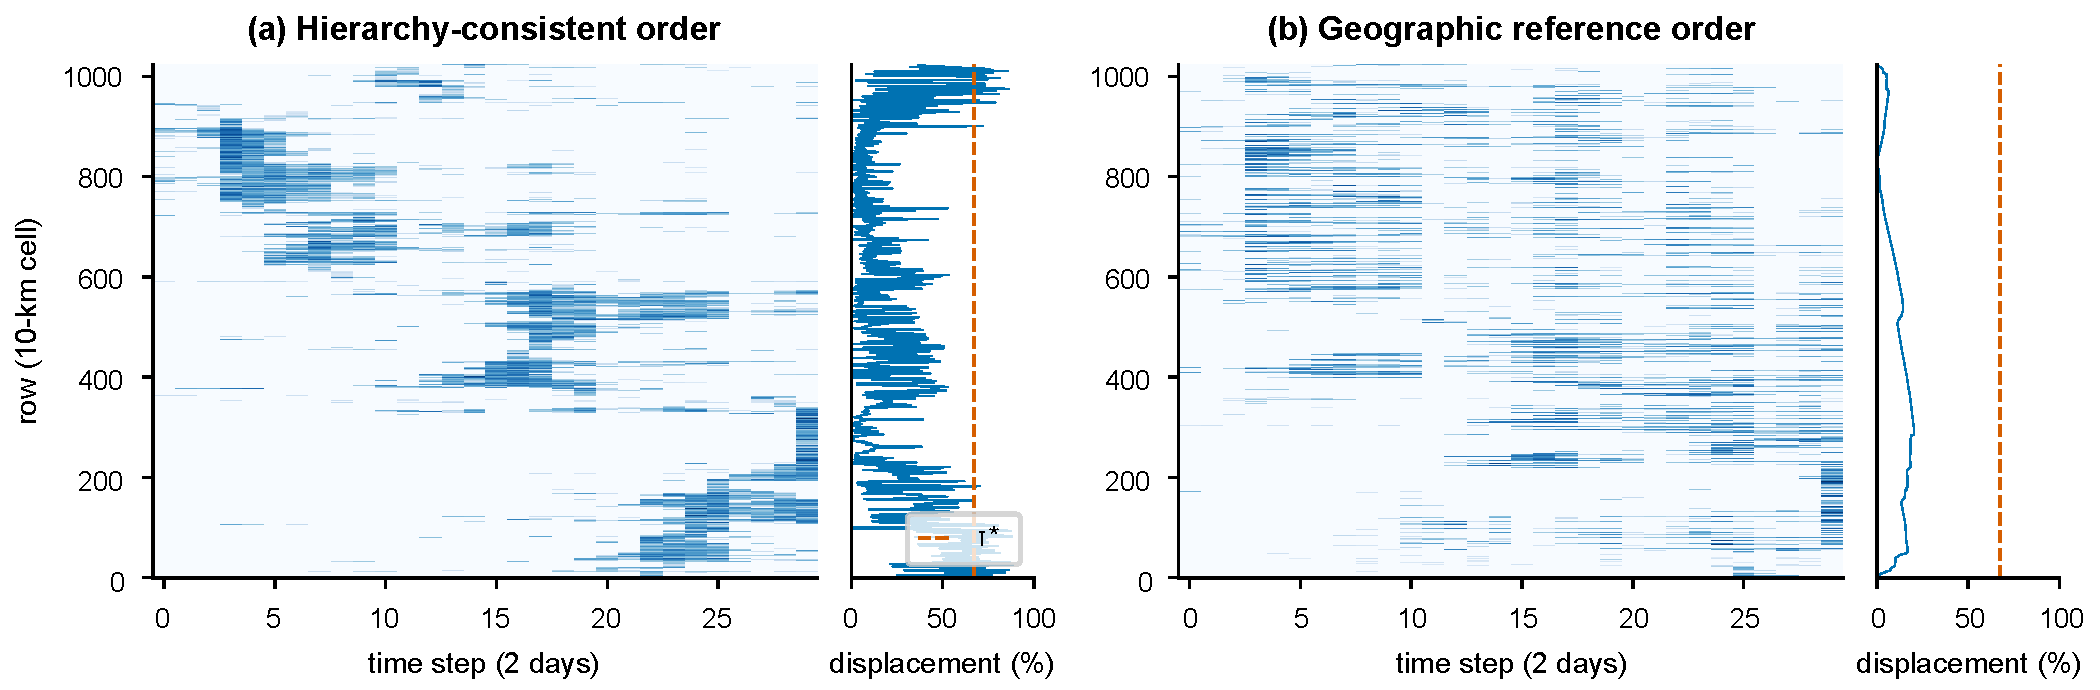
\includegraphics[width=\linewidth]{figures/Supplement_Dendrogram_Transfer.pdf}
\caption{Position certification for a clustering hierarchy of 1024 active wildfire cells. The same 30 two-day $\log(1+\mathrm{FRP})$ observations are arranged in dendrogram-consistent optimal leaf order (a) and in geographic reference order (b). Blue encodes signal magnitude; each cell occupies one row. Side panels show absolute displacement from the cell's principal-axis geographic reference, normalized by 1024 rows. The dashed line marks the hierarchy-constrained optimum $\tau^*\approx67.29\%$ (computed to 0.25 row). Observed maxima are 88.23\% for OLO and 20.55\% for geographic sorting, the free-packing optimum. Their separation distinguishes ordering choice from the additional cost imposed by hierarchy.}
\label{fig:s_dendrogram_transfer}
\end{figure}

The positional certificate extends to clustering hierarchies in dense temporal displays. Figure~\ref{fig:s_dendrogram_transfer} arranges 1024 active 10-km wildfire cells~\cite{Franke:2021:1DP}, each as one row containing 30 two-day $\log(1+\mathrm{FRP})$ observations. Average-linkage clustering of centered, unit-normalized temporal signals defines the dendrogram; optimal leaf ordering (OLO) groups similar signals within its legal orders. Reference positions project cell locations onto the principal geographic axis and span row centers $0.5$--$1023.5$. Both panels contain the same observations and use identical row widths and color mapping.

OLO groups temporally similar activity into visible bands but displaces some cells by 88.23\% of display height. Positional diagnosis over all dendrogram-consistent orders gives $\tau^*/n\approx67.29\%$, where $n=1024$. The approximately 20.94-percentage-point gap separates the chosen ordering's displacement from the minimum imposed by this hierarchy: changing the leaf-ordering algorithm can improve position, while subtree contiguity still prevents accurate geographic placement.

Geographic sorting removes the contiguity constraints and attains $\tau_{\free}/n=20.55\%$. Equal-width rows fill the canvas, so nonuniform geographic references still incur packing cost. The hierarchy contributes the additional $H/n=(\tau^*-\tau_{\free})/n\approx46.73\%$ of display height, or 46.73 percentage points beyond packing. Together with the mirror control, this distinguishes two sources of positional ambiguity: distances alone do not fix absolute references, and a fixed hierarchy can obstruct those references even under optimal positional ordering. The row experiment transfers positional diagnosis to a 1024-leaf clustering tree; the merge-tree experiments quantify scalar correction and relaxation costs. Supplement S3 gives the numerical precision and retained records.


\subsection{Three-dimensional inputs}
\begin{figure}[H]
\centering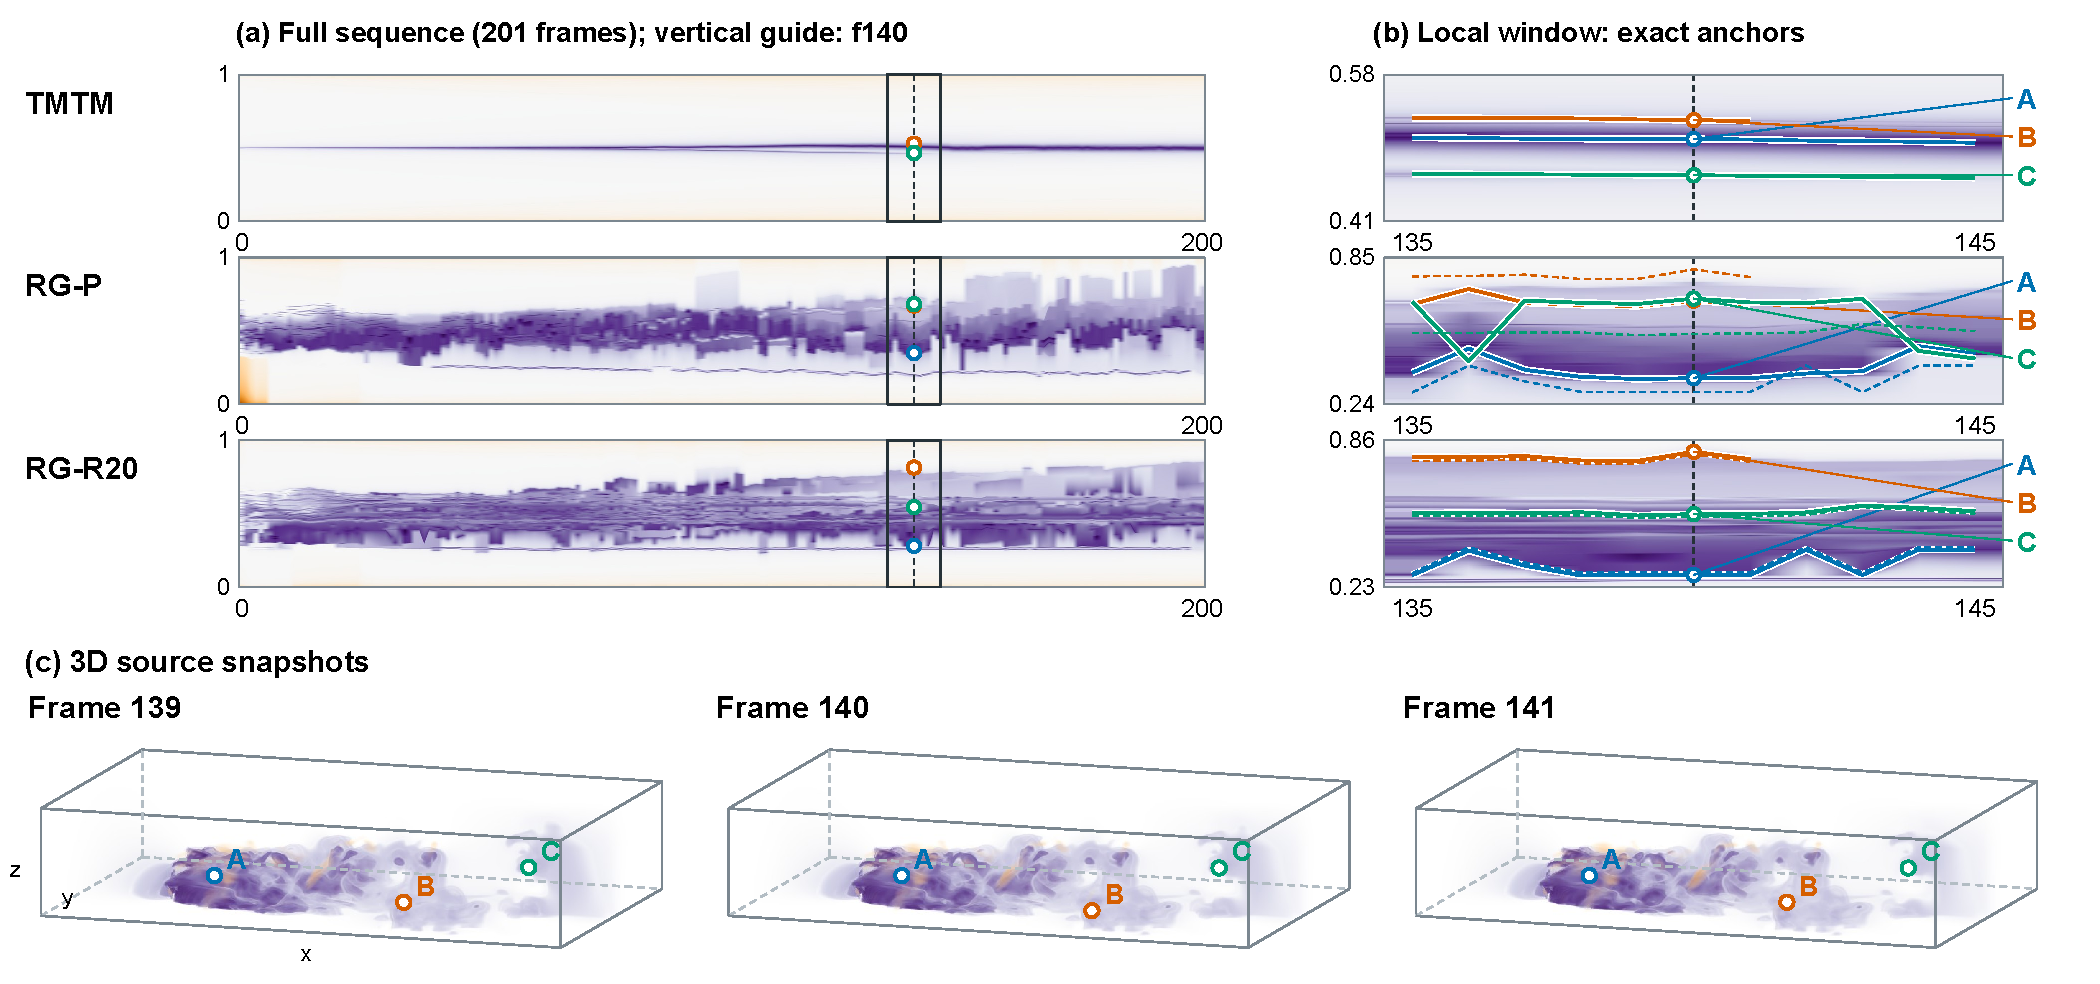
\includegraphics[width=\linewidth]{figures/Supplement_Tangaroa_Comparison.pdf}
\caption{Tangaroa feature correspondence: all 201 original-grid frames at fixed 10\% persistence. Complete TMTM/P/R20 maps (left) link to frames 135--145 (right); tracks $A=432$, $B=462$, $C=388$ use exact saved anchors and dashed RG references. Baseline and RG ordinates retain their distinct meanings. Bottom: cached full-volume views at frames 139--141, with domain boxes and true extrema projected through one shared oblique orthographic camera. Preview layers use 4096 rows; errors use complete 131072-row profiles. At frame 140, P/R maximum displacement is 14.76\%/1.02\%, and R incurs 13.75\% NMLE. Maps and volumes use the retained purple--white--orange speed transfer function over $[0,2]$. Temporal transitions interpolate saved profiles for display only; anchors, input volumes, and evaluation samples are unchanged.}
\label{fig:s_full_volume3d}
\end{figure}

\begin{figure}[H]
\centering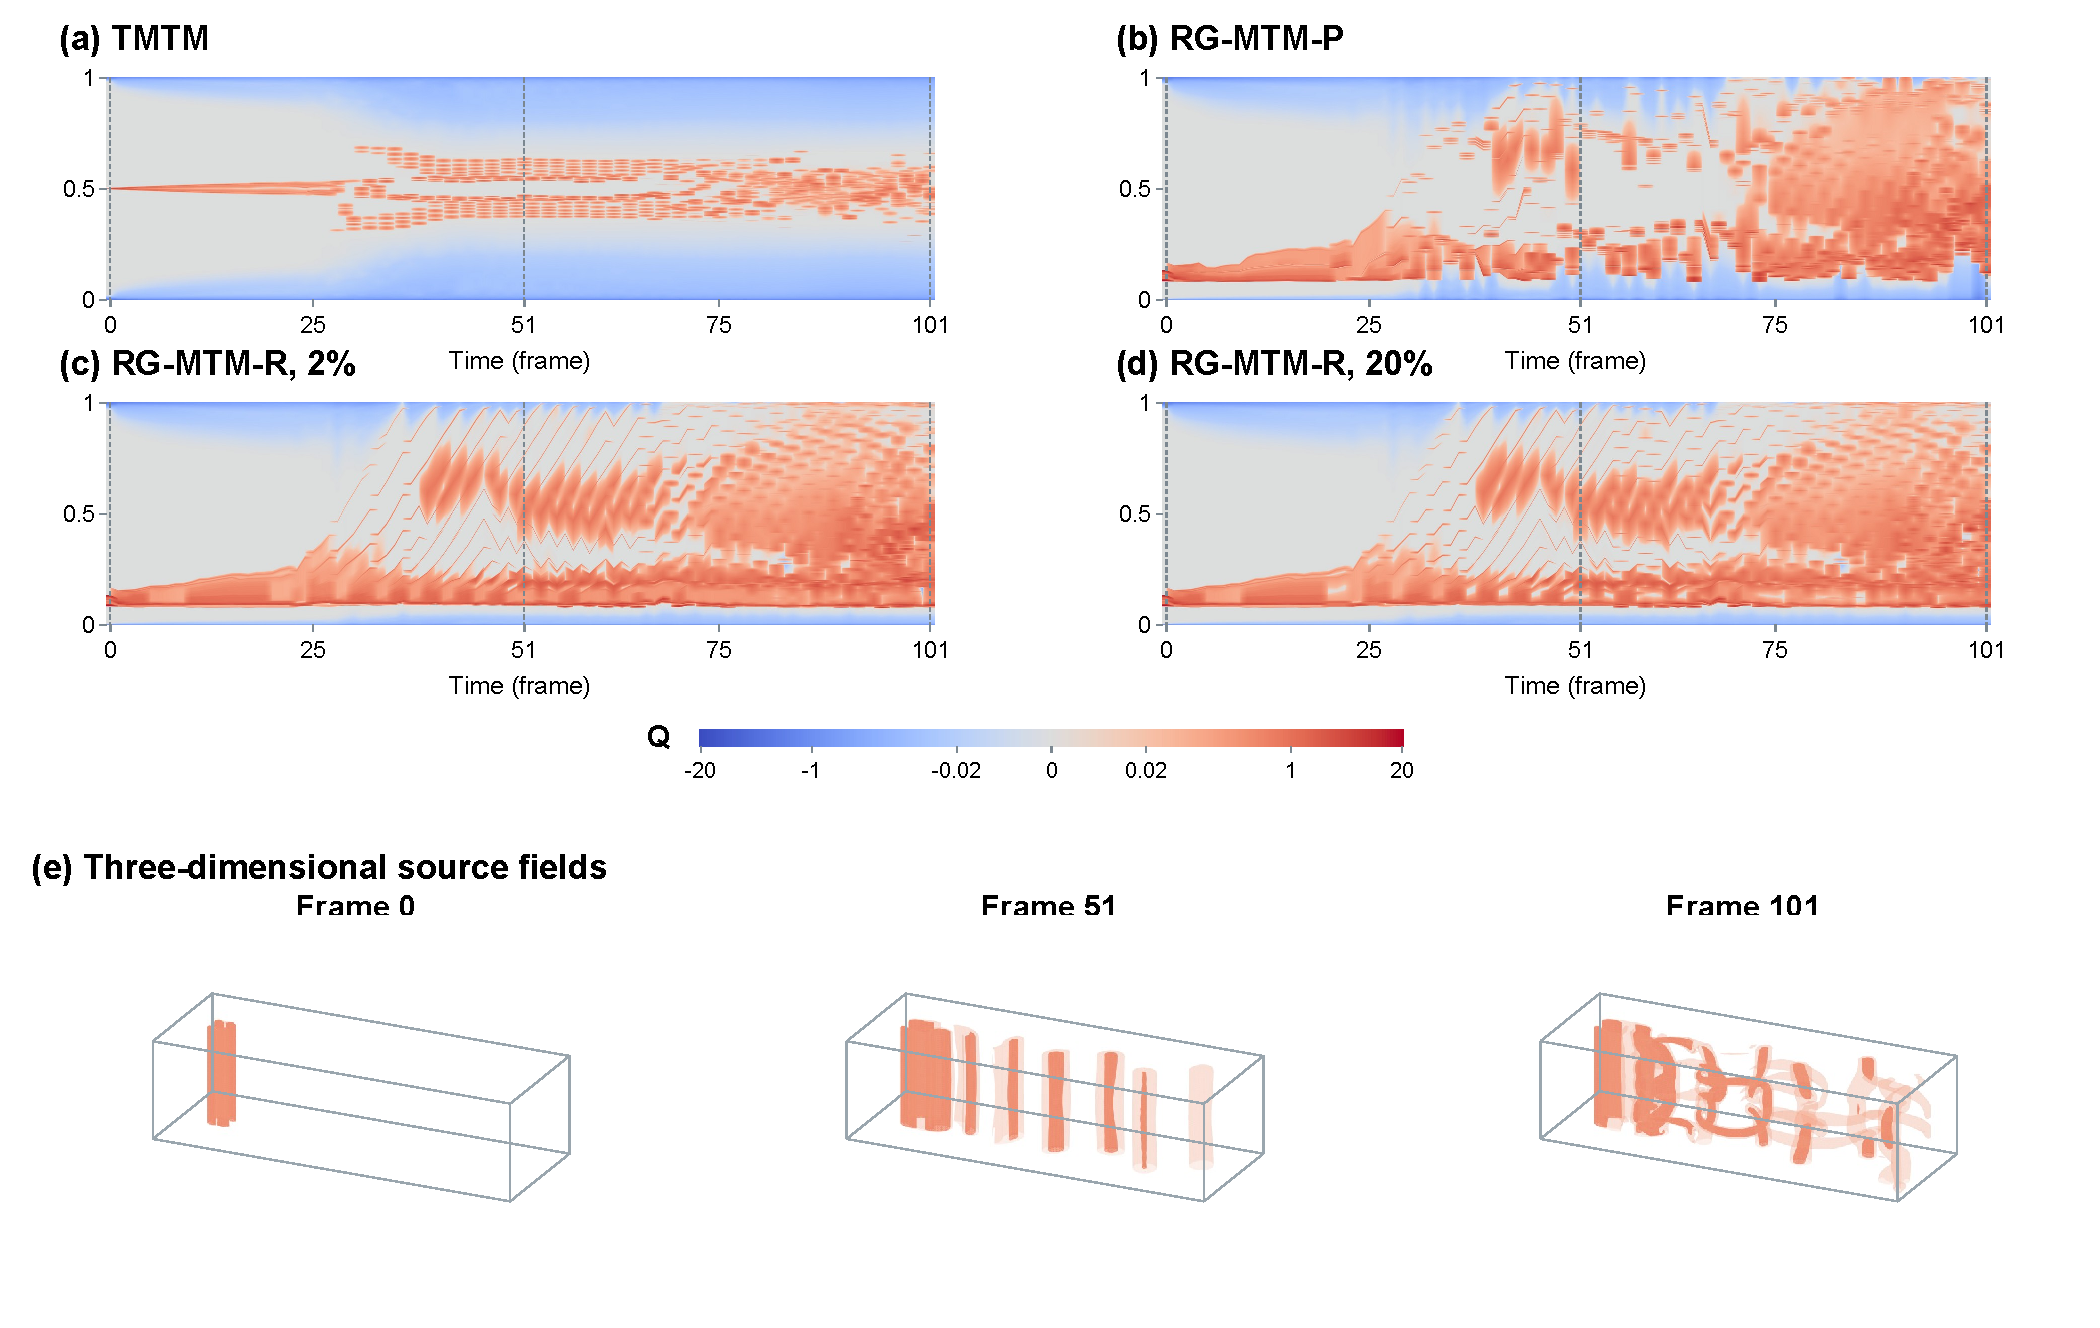
\includegraphics[width=\linewidth]{figures/Supplement_Cylinder_Comparison.pdf}
\caption{Cylinder: 102 original-grid three-dimensional $Q$ fields. (a)--(d) Saved scalar maps for TMTM, P, R2, and R20; TMTM uses a native ordinate, while RG uses normalized physical $x$ reference position. Dashed guides locate frames 0, 51, and 101. The common symmetric-log colour scale is linear within $\pm0.02$; the revised raster integrates complete stored profiles vertically rather than selecting 2048 rows. Temporal colour transitions are display interpolation; metrics use the original arrays. (e) Three-dimensional source isosurfaces at $Q=0.1$ (translucent) and $0.5$ (solid), with identical physical aspect, orthographic camera, and domain frame. They show the source $Q$ before persistence simplification; maps use the shared simplified inputs and their stated scalar fillings.}
\label{fig:s_full_cylinder}
\end{figure}

\bibliographystyle{abbrv-doi-narrow}\bibliography{refs}
\end{document}
